

\documentclass[a4paper,twoside,openright,titlepage,
               headinclude,,footinclude,BCOR5mm,
               numbers=noenddot,cleardoublepage=empty,
               tablecaptionabove]{scrreprt}
              
\usepackage[T1]{fontenc}
\usepackage[utf8]{inputenc}
\usepackage[english]{babel}
\usepackage{amsmath,amssymb}
\usepackage{indentfirst}
\usepackage[style=philosophy-modern,hyperref]{biblatex}
\usepackage{chngpage}
\usepackage{calc}
\usepackage{listings}
\usepackage{graphicx}
\usepackage{subfig}
\usepackage{lipsum}
\usepackage{shapepar}
\usepackage{pifont}
\usepackage[eulerchapternumbers,subfig,beramono,eulermath,pdfspacing,listings]{classicthesis}
\usepackage{arsclassica}
\usepackage{microtype}
\usepackage{classicthesis}
\usepackage{comment}
\usepackage{makeidx}
\usepackage[tight,english]{minitoc}
\usepackage{mathtools,amsthm,amsfonts,amssymb}
\usepackage{bm}
\usepackage{braket}
\usepackage{booktabs}
\usepackage{enumitem}
    \renewcommand{\labelenumi}{(\roman{enumi})}
\usepackage{slashed}
\usepackage{acronym}
    \acrodef{KMS}[KMS]{Kubo-Martin-Schwinger}
    \acrodef{GNS}[GNS]{Gelfand-Naimark-Segal}
\usepackage{epigraph}
    \renewcommand{\textflush}{flushepinormal}
    \renewcommand{\epigraphflush}{flushright}
    \setlength{\epigraphwidth}{17em}
    \setlength{\afterepigraphskip}{3\baselineskip}
\usepackage{simplewick}
\usepackage{comment}
\usepackage{tikz}
    \usetikzlibrary{decorations.markings}

% ********************************************************************
% Personal commands
% ******************************************************************** 
\newcommand{\myTitle}{R for data science}
\newcommand{\mySubtitle}{}
\newcommand{\myName}{Gennaro Tedesco}

%% some more newcommands
\newcommand{\ie}{i.\,e.}
\newcommand{\Ie}{I.\,e.}
\newcommand{\eg}{e.\,g.}
\newcommand{\Eg}{E.\,g.} 


\DeclareRobustCommand*{\clsname}[1]{{\normalfont\sffamily#1}}
\DeclareRobustCommand*{\pkgname}[1]{{\normalfont\sffamily#1}}
\DeclareRobustCommand*{\optname}[1]{{\normalfont\ttfamily#1}}
\DeclareRobustCommand*{\cmdname}[1]{\mbox{\lstinline[basicstyle=\normalsize\ttfamily]!\\#1!}}
\DeclareRobustCommand*{\classicthesis}{Classic\-Thesis}
\DeclareRobustCommand*{\arsclassica}{{\normalfont\sffamily ArsClassica}}


% ********************************************************************
% Hyper-references
% ******************************************************************** 
\newcommand{\mail}[1]{\href{mailto:#1}{\texttt{#1}}}

% ********************************************************************
% Graphics
% ********************************************************************
\graphicspath{{Graphics/}}


% ********************************************************************
% Code
% ********************************************************************
\definecolor{lightergray}{gray}{0.99}

\lstset{language=[LaTeX]Tex,
     keywordstyle=\color{RoyalBlue},
     basicstyle=\small\ttfamily,
     commentstyle=\color{Emerald}\ttfamily,
     stringstyle=\rmfamily,
     numberstyle=\scriptsize,
     showstringspaces=false,
     breaklines=true,
     frame=lines,
     backgroundcolor=\color{lightergray},
     flexiblecolumns=true,
     escapeinside={�*}{*�},
     firstnumber=last,
} 

\newcommand{\meta}[1]{$\langle${\normalfont\itshape#1}$\rangle$}

\lstset{	morekeywords=%
    {ProvidesPackage,RequirePackage,areaset,ifthenelse,%
     chapterNumber,undefined,boolean,DeclareRobustCommand,%
     spacedallcaps,textssc,MakeTextUppercase,lehead,%
     microtypesetup,textls,spacedlowsmallcaps,MakeTextLowercase,%
     sodef,allcapsspacing,lowsmallcapsspacing,thesection,%
     color,headmark,rohead,headfont,pnumfont,titleformat,%
     part,partname,thepart,chapter,thechapter,titlerule,%
     subsection,thesubsection,subsubsection,thesubsubsection,%
     paragraph,theparagraph,descriptionlabel,titlespacing,%
     formatchapter,textcolor,clearscrplain,rofoot,labelitemi,
     captionsetup,hypersetup}}

\lstnewenvironment{code}% 
   {\setkeys{lst}{columns=fullflexible,keepspaces=true}%
   \lstset{basicstyle=\small\ttfamily}}{}


% ********************************************************************
% Bibliography
% ******************************************************************** 
\bibliography{Bibliography}

\defbibheading{bibliography}{%
\cleardoublepage
\manualmark
\phantomsection
\addcontentsline{toc}{chapter}{\tocEntry{\bibname}}
\chapter*{\bibname\markboth{\spacedlowsmallcaps{\bibname}}
{\spacedlowsmallcaps{\bibname}}}}

\renewcommand*{\nameyeardelim}{\addcomma\space}


\makeindex

% -------- new commands defined below -----------
\newcommand{\alg}[1]{\mathcal{A}\left(#1\right)}
\newcommand{\R}{\mathbb{R}}
\newcommand{\C}{\mathbb{C}}
\newcommand{\Z}{\mathbb{Z}}
\newcommand{\N}{\mathbb{N}}
\newcommand{\I}{\textrm{I}}
\newcommand{\s}{\textrm{S}^1}
\newcommand{\hil}{\mathcal{H}}
\newcommand{\U}[1]{\textrm{U}(#1)}
\newcommand{\bh}{\mathcal{B}(\mathcal{H})}
\newcommand{\vac}{\omega_0}
\newcommand{\vN}{\mathcal{M}}
\newcommand{\dom}[1]{\mathfrak{D}(#1)}
\newcommand{\wed}{\mathcal{W}}
\newcommand{\blank}{(\;{\cdot}\;)}
\newcommand{\poin}{\overline{\mathfrak{P}}}
\newcommand{\loren}{\overline{\mathfrak{L}}}
\newcommand{\conj}[2][3]{{}\mkern#1mu\overline{\mkern-#1mu#2}} % conjugate
\newcommand{\LL}[1]{\textrm{L}^2(#1)}
\newcommand{\LX}{\textrm{LX}}
\newcommand{\dd}{\textrm{d}}
\newcommand{\dummy}{Bla bla bla\ldots} % dummy text to be inserted
\newcommand{\open}[2]{\mathopen{]}#1,#2\mathclose{[}}
\newcommand{\ram}[1]{\pi_{\textrm{R}}(\psi(#1))}
\newcommand{\im}[1]{\mathfrak{Im}(#1)}


%new command for the underbrace
\newdimen{\underlen}%
\newcommand{\under}[2]{%
\underset{\settowidth{\underlen}{$#2$}%
\makebox[\underlen]{%
\leftarrowfill$\scriptstyle\;#1\;$\rightarrowfill}}{#2}}


\definecolor{navy}{rgb}{0,0.25,0.65}
\newcommand{\navy}[1]{\textcolor{navy}{#1}}

% some awesome delimiters
\DeclarePairedDelimiter{\abs}{\lvert}{\rvert} % use also the *-version
\DeclarePairedDelimiter{\comm}{[}{]} % use also the *-version
\DeclarePairedDelimiter{\ant}{\{}{\}} % use also the *-version
\DeclarePairedDelimiter{\wick}{:}{:} % use also the *-version
\DeclarePairedDelimiter{\norm}{\lVert}{\rVert} % use also the *-version
\DeclarePairedDelimiter{\scal}{(}{)}

% hyphenation patterns
\hyphenation{di-men-sio-nal}
\hyphenation{va-lues}
\hyphenation{po-si-ti-ve}
\hyphenation{e-ner-gy}
\hyphenation{se-pa-ra-ting}
\hyphenation{Hil-bert}
\hyphenation{to-po-lo-gy}
\hyphenation{va-cuum}
\hyphenation{ma-the-ma-ti-cal}
\hyphenation{ge-ne-ra-ted}
\hyphenation{sui-ta-ble}
\hyphenation{ac-cor-din-gly}
\hyphenation{eve-ry}
\hyphenation{ge-ne-ral}
\hyphenation{o-pe-ra-tors}
\hyphenation{com-mut-ing}
\hyphenation{sa-tis-fies}
\hyphenation{mo-dels}
\hyphenation{dif-fe-rent}
\hyphenation{mo-du-lar}
\hyphenation{in-te-re-sting}
\hyphenation{pa-ra-me-ter}
\hyphenation{mo-du-lar}
\hyphenation{ta-king}


% some awesome math operators
\DeclareMathOperator{\Diff}{Diff}
\DeclareMathOperator{\Det}{det}
\DeclareMathOperator{\e}{e}
\DeclareMathOperator{\tr}{tr}
\DeclareMathOperator{\ad}{Ad}
\DeclareMathOperator{\aut}{Aut}
\DeclareMathOperator{\rot}{rot}
\DeclareMathOperator{\dm}{dim}
\DeclareMathOperator{\OPE}{OPE}


% equations labelled within the sections
\numberwithin{equation}{section}


%newtheoremstyle
\newtheoremstyle{classicthm}
{15pt}
{15pt}
{\rmfamily}
{}
{\itshape}
{:}
{.5em}
{}

\theoremstyle{classicthm}
\newtheorem{theorem}{Theorem}[section]
\newtheorem*{definition}{Definition}
\newtheorem*{example}{Example}
\newtheorem*{property}{Property}
\newtheorem*{proposition}{Proposition}
\newtheorem{corollary}[theorem]{Corollary}
\newtheorem*{lemma}{Lemma}



\begin{document}
\pagenumbering{roman}
\pagestyle{plain}
% !TEX TS-program = pdflatex
% !TEX root = ../ArsClassica.tex

%*******************************************************
% Titlepage
%*******************************************************
\begin{titlepage}
\pdfbookmark{Titlepage}{Titlepage}
\changetext{}{}{}{((\paperwidth  - \textwidth) / 2) - \oddsidemargin - \hoffset - 1in}{}
    \begin{center}
        \large  

        \hfill

        \vfill

        \begingroup
            \color{Maroon}\spacedallcaps{\myTitle} \\ \bigskip
        \endgroup

        %\spacedallcaps{\myName}

        \vspace{2cm}

        
\includegraphics[scale=3]{Graphics/logo} \\ 
        
        \vspace{3cm}
        Dissertation\\ 
        zur Erlangung des mathematisch-naturwissenschaftlichen
        Doktorgrades \\``Doctor rerum naturalium''der Georg-August-Universit\"at 
        G\"ottingen  
        
        \bigskip
        im Promotionsprogramm ProPhys\\ 
        der Georg-August University School of Science (GAUSS) 
        
        \vspace{1cm}       
        vorgelegt von\\
        \myName \\
        aus Eboli, Italy\\
        
        \vspace{1cm}
        
        G\"ottingen, 2014
        %\mySubtitle \\ \medskip   
        %\myDegree \\
        %\myDepartment \\ \medskip       
        
        %\myFaculty \\ \medskip
        
        %\myUni \\ \bigskip

        %\myTime\ %-- \myVersion

        \vfill               

    \end{center}        
\end{titlepage} 
\thispagestyle{empty}

\hfill

\vfill


\bigskip

\noindent \spacedallcaps{Betreungsausschuss:}

\medskip
\noindent Prof. Dr. Karl-Henning Rehren, Institute for Theoretical Physics\\
Prof. Dr. Dorothea Bahns, Institute of Mathematics\\

\bigskip 
\noindent \spacedallcaps{Mitglieder der Pr\"ufungskommission:}

\medskip
\noindent Referent: Prof. Dr. Karl-Henning Rehren \\
Korreferentin: Prof. Dr. Laura Covi \\

\bigskip 
\noindent \spacedallcaps{Weitere Mitglieder der Pr\"ufungskommission:}

\medskip
\noindent 
Prof. Dr. Dorothea Bahns, Institute of Mathematics\\
Prof. Dr. Andreas Honecker, External Member\\
Prof. Dr. Thomas Schick, Institute of Mathematics\\
Jun. Prof. Dr. Steffen Schumann, II. Institute of Physics



\vspace{2cm}
Tag der m\"undlichen Pr\"ufung: 
\cleardoublepage%*******************************************************
% Dedication
%*******************************************************
\thispagestyle{empty}
%\phantomsection 
\pdfbookmark[1]{Dedication}{Dedication}

\vspace*{3cm}

\begin{center}
    If people do not believe that mathematics 
    is simple\\ it is only because they do not
    realise how complicated life is.\\ \medskip
    --- John von Neumann    
\end{center}

\cleardoublepage%*******************************************************
% Abstract
%*******************************************************
%\renewcommand{\abstractname}{Abstract}
\pdfbookmark[1]{Abstract}{Abstract}
\begingroup
\let\clearpage\relax
\let\cleardoublepage\relax
\let\cleardoublepage\relax

\chapter*{Abstract}
The following thesis deals with the modular theory of 
Fermi fields in low dimensions; in particular, making 
use of the algebraic approach to quantum field theory,
we have investigated the behaviour of two-dimensional 
theories which split into two separate copies of chiral
fields, each one of them depending on one lightray variable 
at a time only.

The remarkable result we have found is the existence of 
a vacuum preserving isomorphism $\beta$ connecting the 
vacuum states between the algebra of $N$ Fermi fields 
localised in one single interval $\I$ and the algebra 
of one Fermi field localised in $N$ disjoint intervals 
$\textrm{E}_N=\I_1\cup\ldots\cup \I_N$. Since this 
map preserves the vacuum states, it therefore intertwines 
the respective modular groups; as a result, the modular 
automorphism flow for a Fermi field localised in several 
intervals turns out to mix the field among different 
points, with the mixing itself being described through 
suitable differential equations. Moreover, using the fact that
Wick products are as well preserved, one can even embed 
via $\beta$ the sub-theories of local observables,
as currents and the stress-energy tensor. Consequently,
since the isomorphism $\beta$ is multi-local, a 
new class of multi-local gauge transformations and 
diffeomorphisms arise. 

Interestingly enough, such characterisation of the 
modular group for multi-local algebras was already 
presented by \cite{CH:2009} using different
techniques, and so far it is a special feature of 
free Fermi fields only (although outlooks of generality
are fascinating to investigate).

\bigskip
The isomorphism that we have found is deeply related to 
the split property and the way fields transform under 
diffeomorphism covariance. In particular, it only differs 
from the action of diffeomorphisms by a gauge transformation,
whose features we have characterised in the cases at hand,
namely for the local algebras of Fermi fields, currents and 
stress-energy tensor.


\vfill

\pdfbookmark[1]{Zusammenfassung}{Zusammenfassung}
\chapter*{Zusammenfassung}
Die folgende Doktorarbeit befasst sich 
mit der Modulartheorie von Fermifeldern in niedrigen Dimensionen;
insbesondere untersuchen wir das Verhalten der chiralen Felder,
nachdem Felder in zwei Dimensionen 
in zwei ein-dimensionale Lichtstrahlkomponenten 
zerlegt worden sind. Wir wenden den algebraischen
Zugang zur Quantenfeldtheorie an, in dem man sich mit 
lokalen Algebren befasst. 

Wir finden einen Isomorphismus $\beta$ zwischen 
der Algebra von $N$ Fermifeldern, die in einem einzelnen Interval
$\I$ lokalisiert sind, und der Algebra eines Fermifelds, 
das in mehreren verschieden Intervallen $\textrm{E}_N
=\I_1\cup\ldots\cup \I_N$ lokalisiert ist, der den Grundzustand
erh\"alt. Daher verkn\"upft dieser die 
korrespondierenden Grundzustandmodulargruppen. Weil 
dieser Isomorphismus nicht-lokal ist, ergibt sich eine Mischung 
f\"ur die Modulargruppe der Multi-Interval-Algebra, 
die das Feld in verschiedenen Punkten in den unterschiedlichen 
Intervallen mischt.

\bigskip
Diese Characterisierung der Modulargruppen f\"ur die 
Multi-Interval-Algebra ist nur f\"ur freie chirale Fermifelder bekannt. 
Da dieser Isomorphismus auch Wick Produkte erh\"alt, k\"onnen auch
lokale Observablen, wie die Str\"ome und der Energie-Impuls-Tensor, 
damit eingebettet werden. Wegen dieses Merkmals kann man 
multi-lokale Eichsymmetrien und Diffeomorphismen generieren,
deren Verhalten wir auch untersucht haben.

\bigskip 
Der Isomorphismus, den wir gefunden haben, setzt sich interessanterweise
zusammen aus dem Split-Isomorphismus einer geeigneten Wirkung
der Diffeomorphismen und einer Eichtransformation. 
Das gleiche Verhalten kann man auch auf die 
Untertheorien der Str\"omen und des Energie-Impuls-Tensors 
einschr\"anken, was wir uns im letzten Kapitel angesehen haben.


\endgroup			

\vfill
\pagestyle{scrheadings}
\dominitoc
\cleardoublepage%*******************************************************
% Table of Contents
%*******************************************************
%\phantomsection
\pdfbookmark[1]{\contentsname}{tableofcontents}
\setcounter{tocdepth}{2} % <-- 2 includes up to subsections in the ToC
\setcounter{secnumdepth}{3} % <-- 3 numbers up to subsubsections
\manualmark
\markboth{\spacedlowsmallcaps{\contentsname}}{\spacedlowsmallcaps{\contentsname}}
\tableofcontents 
\automark[section]{chapter}
\renewcommand{\chaptermark}[1]{\markboth{\spacedlowsmallcaps{#1}}{\spacedlowsmallcaps{#1}}}
\renewcommand{\sectionmark}[1]{\markright{\thesection\enspace\spacedlowsmallcaps{#1}}}
%*******************************************************
% List of Figures and of the Tables
%*******************************************************
\clearpage

\begin{comment}
\begingroup 
    \let\clearpage\relax
    \let\cleardoublepage\relax
    \let\cleardoublepage\relax
    %*******************************************************
    % List of Figures
    %*******************************************************    
    %\phantomsection 
    %\addcontentsline{toc}{chapter}{\listfigurename}
    \pdfbookmark[1]{\listfigurename}{lof}
    \listoffigures

    \vspace*{8ex}

    %*******************************************************
    % List of Tables
    %*******************************************************
    %\phantomsection 
    %\addcontentsline{toc}{chapter}{\listtablename}
    \pdfbookmark[1]{\listtablename}{lot}
    \listoftables
        
    \vspace*{8ex}
%   \newpage
    
    %*******************************************************
    % List of Listings
    %*******************************************************      
	  %\phantomsection 
    %\addcontentsline{toc}{chapter}{\lstlistlistingname}
    \pdfbookmark[1]{\lstlistlistingname}{lol}
    \lstlistoflistings 

    \vspace*{8ex}
       
    %*******************************************************
    % Acronyms
    %*******************************************************
    %\phantomsection 
    \pdfbookmark[1]{Acronyms}{acronyms}
    \markboth{\spacedlowsmallcaps{Acronyms}}{\spacedlowsmallcaps{Acronyms}}
    \chapter*{Acronyms}
    \begin{acronym}[UML]
        \acro{DRY}{Don't Repeat Yourself}
        \acro{API}{Application Programming Interface}
        \acro{UML}{Unified Modeling Language}
    \end{acronym}                     
\endgroup
\end{comment}
\cleardoublepage
\cleardoublepage%*******************************************************
% Abstract
%*******************************************************
%\renewcommand{\abstractname}{Abstract}
\pdfbookmark[1]{Introduction}{Introduction}
\begingroup
\let\clearpage\relax
\let\cleardoublepage\relax
\let\cleardoublepage\relax

 \addcontentsline{toc}{section}{Introduction}
 \chapter*{Introduction}
 The main theoretical ingredient of algebraic quantum field
 theory is the concept of field, which is supposed to
 implement the principle of locality. Observables, identified
 with the quantities that can be experimentally measured in a 
 laboratory, must satisfy Einstein causality and additional
 physical requirements that are seen to be realised in 
 nature. Fields therefore appear as the building blocks
 in order to construct such observables and, though they
 may themselves be observables, they need not to. The idea 
 lying at the basis of quantum field theory is the 
 assignment of fields to each space-time region, where
 events are supposed to take place. This reflects into 
 the assignment of a net of algebras onto the Minkowski
 space; physical measurements correspond, roughly speaking,
 to states on the algebras and all the most important physical
 quantities experimentalists are interested in can usually
 be traced back to the evaluations of scalar product or 
 particular combinations thereof, as for example correlations
 functions and scattering amplitudes: notable in this 
 sense is the Lehmann-Symanzik-Zimmermann formula reducing 
 scattering amplitudes to time-ordered correlations functions
 and their poles.
 
 The algebraic approach to quantum field theory deals with
 the mathematical properties of all these ingredients 
 from the point of view of operator algebras. 
 A marvelous walkthrough these aspects is provided by 
 \cite{Haag} and \cite{roberts:2004} who give complete
 explanations of why this is a necessary issue. The developement
 of such a formalism is the key tool to the understanding of
 quantum field theory itself and encodes almost all the 
 features that we find as realised in nature. Many results
 have been achieved thanks to the possibility to handle 
 these mathematical tools, especially after very important
 insights by Takesaki and Tomita, \cite{Borchers:1999},
 \cite{Tak:1970}, \cite{TAKII:2002}, who reduced the origin
 of space-time symmetries to abstract properties of von 
 Neumann algebras, opening a brand new research field
 consequently.
 
 \bigskip 
 A very important role in physics is played by systems 
 which exhibit special symmetries, because this characteristic
 helps a lot to reduce their complexity. In particular 
 we have been concerned with models being symmetric under
 conformal transformations, that is the set of transformations 
 preserving the angles in the Minkowski space-time.   
 In low dimensions, namely two, this symmetry happens to reduce to
 very strict requirements with a well-known mathematical structure
 described by the Virasoro algebra. Investigation of the 
 properties of such algebras leads to amazing results
 and progresses in the area. The Virasoro generators are 
 moreover the modes of the stress-energy tensor, which 
 generates space-time diffeomorphisms of the theory. 
 As a consequence, a two-dimensional conformal field
 theory is basically a quantum field theory endowed with
 a stress-energy tensor whose generators must satisfy 
 specific algebraic properties and commutation relations.
 Also, the theory contains a special class of fields,
 the ``primary fields'', whose transformations properties 
 are very much related to how these fields commute with the 
 stress-energy tensor itself.
 
 Interestingly enough, conformal symmetries can be found
 very often in actual physical systems. Most of the 
 times this goes along with scaling invariance and,
 although the two properties do not coincide, they 
 are nevertheless very often interchanged. Models 
 with no proper scale dimensions, as for example
 massless models, are usually conformally invariant 
 and form the prototypes we can look at, not to mention 
 the huge amount of results, models and features carried
 by string theory, which is the straightforward 
 application of conformal field theory. However, within 
 the already mentioned two-dimensional models, 
 a special class is given
 by the so called chiral theories, a group of models
 where the fields only depend on the ``light-cone'' variables
 $x^{\pm}\coloneqq x^0\pm x^1$.
 Those theories decouples into two copies of 
 singular theories, either of them being concerned with 
 the one variable $x^+$ or $x^-$, respectively. This 
 means that the whole business reduces to a one-dimensional 
 theory, and the original model can be reconstructed eventually
 taking the tensor product of the two one-dimensional copies. 
 The term chiral becomes then synonym of one-dimensional 
 world living on a light-ray:
 \begin{figure}[htbp]
 \centering 
 \begin{tikzpicture}[scale=1.5]
 \draw [->] (-1,0) --(1,0);
 \draw [->] (0,-1) --(0,1);
 \draw [dashed] (-0.75,-0.75) -- (0.75,0.75);
 \draw [dashed] (0.75,-0.75) -- (-0.75,0.75);
 \node at (1,-0.2) {\footnotesize $x^1$};
 \node at (-0.2,1) {\footnotesize $x^0$};
 \node[rotate around={45:(-0.6,2)}] 
 {\footnotesize $x^+$};
 \node[rotate around={-45:(0.5,1.8)}] 
 {\footnotesize $x^-$};
 \end{tikzpicture}
 \end{figure}
 
 \noindent Each real line supports both the time-like 
 property (positivity of the energy) and the
 space-like commutativity (causality). Moreover 
 the real line can be taken onto the unit circle (minus 
 a point) via the Cayley transformations and thus 
 we shall basically be concerned with fields living 
 on a circle, 
 where the conformal transformations acquire the 
 form of general diffeomorphisms.
 
 \bigskip 
 Going back to the mathematical questions, we have 
 already stated that a revolutionising result 
 was found by Tomita and Takesaki and undergoes 
 the name of modular theory. Starting with a von 
 Neumann algebra and a cyclic and separating state 
 one can automatically construct an inner group of 
 automorphisms $\sigma_t$ whose explicit form 
 depends on the algebra itself and on the state 
 provided. In some special case, where the algebras
 are generated by local fields localised in particular 
 space-time regions, this group of automorphisms 
 happens to coincide with some symmetry group 
 occurring in physics (Lorentz boosts, dilations). 
 This result opens a brand new horizon of questions, 
 because it seems that the space-time symmetries lie 
 behind the physical content, back in the algebraic 
 properties of the quantities at hand. It is tempting
 to generalise such results and further investigate them.
 The main content of this thesis is exactly modular theory 
 for Fermi fields in one dimension: in particular, we have 
 been looking at fields localised in disjoint intervals,
 trying to derive and explain the features of their modular 
 theory. It turns out that whenever we choose the fields 
 to be localised in many disjoint intervals, the action of 
 the modular group 
 introduces a mixing among those different intervals on top 
 of a geometric action moving the points, 
 (\cite{CH:2009}, \cite{LMR:2009}). 
 This result can be traced back to the existence of 
 a vacuum preserving isomorphism moving the fermions 
 all around the circle \cite{Rehren:2012wa}. We have
 widely exploited this feature considering different 
 representations of the algebras and different situations 
 at hand, varying the geometric positions of the intervals 
 and comparing the new results to previous statements.
 Besides modular theory itself, this work gave us a 
 deeper understanding of how Fermi fields behave on the
 circle.
 
 Also, since products of Fermi fields generate observables
 as currents and the stress-energy tensor, these subtheories 
 can be embedded via the mentioned isomorphism and new 
 characteristics emerge. Currents generate gauge transformations
 which are therefore delocalised all around the circle, as 
 well as new multi-local diffeomorphisms given by the 
 embedded stress-energy tensor. As a consequence, all the
 standard constructions we have for fermions and related 
 models can be rephrased in terms of this new aspect,
 giving rise to a new class of perspectives.
 
 \bigskip 
 As for the  
 organisation of the material, this thesis is divided into 
 different parts. In the beginning we provide the standard 
 description of the mathematical framework lying behind 
 algebraic quantum field theory, following the lines of 
 \cite{Haag}. We introduce the technical aspects of 
 von Neumann algebras and the world of conformal field 
 theory in the field theoretical setting. 
 
 We then move to the analysis of the modular theory for 
 fermions localised in different intervals, 
 showing the new
 aspects together with new insights on the standard 
 constructions. We ought to mention that part of the 
 ideas were triggered by the original work of 
 Casini and Huerta, \cite{CH:2009}, where the authors 
 calculated the modular group for fermions in disjoint 
 intervals using methods coming from density matrices 
 and statistical mechanics. We took their starting point 
 to rephrase everything in the language of algebraic quantum 
 field theory and operator algebras. Other ideas came from
 different works on boson-fermion correspondences, 
 \cite{Ang:2011} as well as others, and we
 tried to contribute attacking the problems from the 
 angle of local quantum physics.
 
 A third part describes the class of models which can 
 be obtained out of Fermi fields, mainly concerning
 currents and their features, in the light of the 
 new background provided. The multi-local features 
 restrict to these subalgebras with the help of suitable 
 gauge transformations, which can be related to the 
 diffeomorphisms covariance in a limpid way.
 
  
\endgroup			

\cleardoublepage

%********************************************************************
% Mainmatter
%*******************************************************
\pagenumbering{arabic}
{\epigraph{The German term ``Nahwirkungsprinzip'' is
            more impressive than the somewhat colourless word 
           ``locality.''}%
           {R. Haag, \emph{Local quantum physics}.}
\part{Preliminaries}
\cleardoublepage%************************************************
\chapter{Introduction to quantum field theory}\label{ch:QFT}
\minitoc\mtcskip
%************************************************

\noindent A rigorous inspection of the behaviour of quantum field theory
showed some common general features which were seen to be 
always realised, no matter the physical system at hand.
Such features have been thus taken as defining properties 
(axioms) of the quantum field theory itself and the study of their 
mathematical properties leads to the characterisation 
of algebraic quantum field theory. We shall introduce such
postulates following the example given by the standard
textbook in this area, namely \cite*{Haag}.

\bigskip
The main objects any physical theory deals with, no matter
whether classical or quantised, are fields $x\mapsto\phi(x)$
(whose mathematical properties have to fulfill the requirements 
of the model at hand).
Their role is to implement the principle of locality; 
\emph{observables} are the quantities that can be directly
reproduced in a laboratory and they can in general be
read off and reconstructed once the field content is assigned.
Fields themselves may also be observables, though they need not to.

%*******************************************************
\section{General postulates: Wightman axioms}
\label{Wightman}
 \begin{enumerate}[label=\Alph*.]
  \item \emph{Fields}:        
        Fields are operator valued distributions on Minkowski space.
        This means that the linear assignment $f\mapsto\phi(f)$ gives
        back an (usually unbounded) operator on some Hilbert space 
        $\hil$ with dense domain $\mathfrak{D}(\phi(f))\subseteq\hil$. 
        The assignment has to be thought as a smearing
        \[
        \phi(f)=\int_{\vN} \dd^4x\,\phi(x)f(x)
        \]
        with $f$ belonging to some suitable functional space $\mathcal{F}$.
        The further assumption $\phi(f)\mathfrak{D}\subset\mathfrak{D}$
        ensures that we may operate arbitrarily many times with fields
        upon vectors $\in\mathfrak{D}$.
  \item \emph{Poincar\'{e} group and transformation properties}: 
        The Hilbert space $\hil$ carries
        a unitary representation $U(g)$ of the covering of the 
        Poincar\'{e} group $\poin$. The spectrum of the energy-momentum
        operators $P^{\mu}$ is contained in the forward light cone
        and this ensures consistency with special relativity,
        $p^2\coloneqq m^2\geq 0, p^0\geq 0$. Moreover, let $\loren\subset\poin = 
        \R^4 \rtimes \loren$ be the Lorentz subgroup of the Poincar\'{e}
        group and let $U(\Lambda,a)$ be a representation of $\poin$
        with $\Lambda\in\loren,\,a\in\R^4$. Fields transform under $\poin$~as
        \[
        U(\Lambda,a)\,(\phi(x))\,U^*(\Lambda,a)= S(\Lambda^{-1})\,
        \phi(\Lambda x+a),\quad S(\Lambda^{-1})\in\,\loren.
        \]
        In a nutshell the choice of $S(\Lambda)$ characterises the
        ``spin'' of the field.
  \item \emph{Hermiticity}: Given a field $\phi(f)$, the theory
	contains also the hermitian conjugate field $\phi(f)^*$ 
	defined so that 
	\[
	\scal{\Phi,\phi(f)\Psi}=\scal{\phi^{\dagger}(\overline{f})\Phi,\Psi}.
	\]
	Fields may be self-adjoint, $\phi(x)=\phi^{\dagger}(x)$ and
	thus $\scal{\Phi,\phi(f)\Psi}=\scal{\phi(\overline{f})\Phi,\Psi}$
	given $\Phi,\Psi$.
  \item \emph{Locality}: If the supports of the test functions $f$ and
	$g$ are space-like to each other, then fields must satisfy either
	of the following commutation relations
	\[
	\comm{\phi(f),\phi(g)}\Psi=0\quad\text{or}\quad
	\ant{\phi(f),\phi(g)}\Psi=0,\quad\Psi\in\mathfrak{D}. 
	\]
        Fields of the former type are called ``bosonic'', whereas
        fields of the latter type are called ``fermionic''. Due
        to Einstein causality observables must commute at space-like
        distances, therefore fermionic fields by themselves cannot be
        observables, whilst bosonic fields may.  
  \item \emph{Vacuum state and completeness}: There exists a unique state 
        $\Omega\in\hil$ invariant under 
        $U(g),\,g\in\poin$. Such a state is referred to as the 
        ``vacuum state''. Also, by acting upon the vacuum with an 
        arbitrary polynomial in the fields $\phi(f)$ one can approximate 
        any operator acting on $\hil$.        
 \end{enumerate}
It turns out that these properties are easily realised by free fields
satisfying linear equations, while constructions in terms of 
interacting fields are very difficult to achieve.

 \begin{definition}
 Let $\Omega$ be the vacuum vector. The vacuum expectation values
 \[
 w^{(n)}(x_1,\ldots,x_n)\coloneqq
 \scal{\Omega,\phi(x_1)\ldots\phi(x_n)\Omega}
 \]
 are called (Wightman) $n$-points correlation functions, though
 they are, more precisely, tempered distributions on $\R^{4n}$.
 \end{definition}
A fundamental result in this respect is the ``reconstruction theorem''
\cite*{Haag}, namely, under some suitable assumptions that we do not 
discuss in here, the whole fields content can be derived out of the 
knowledge of all correlation functions. 

\section{Fermi fields versus Bose fields}
\label{Fermi vs Bose}
As previously stated, fields appearing in nature must satisfy particular
restrictions on the way they commute between each other, this being
express by either commutation or anti-commutation relations. 
Fields of the former kind are referred to as ``Bose fields''
whereas fields of the latter kind are usually referred to as 
``Fermi fields''. In particular, those fields that belong 
to integer ``spin representations'' of the Lorentz group 
(in the sense of $S(\Lambda)$, as we have seen 
before) are Bose fields, while those ones that belong to
half-odd integer representations are Fermi fields. Such
particular feature characterises the spin-statistic
theorem (\cite{Haag}). As a first remark notice
that Bose fields might in principle be already observables, 
because they automatically fulfill Einstein causality; 
on the other hand Fermi fields do not, and observables 
must be constructed as particular combinations
of them (currents and stress-energy tensor, as we will 
show later on). However, we shall show the explicit 
construction of operator algebras based on the above 
commutation relations in the very special case when 
the space-time is one-dimensional, where this has
to be understood as previously mentioned, namely 
as decomposition in terms of light-ray variables.

\bigskip
Let us construct fermionic fields first. Take $\hil$ as 
any Hilbert space of functions with an involution 
$\Gamma\mid(\Gamma f)(x)=\conj{f(x)}$. Through the 
following linear assignment $f\mapsto\psi(f)$, which 
can be thought as an integral smearing, we can construct 
the set
\[
\textrm{CAR}(\hil,\Gamma)\coloneqq
\conj{\set{\psi(f)\mid f\in \mathcal{\hil},\ 
(\Gamma f)(x)=\conj{f(x)}}}_{\norm{\blank}}\,.
\]
The norm of an operator in such a set is uniquely fixed by the relation
$\psi(f)^*=\psi(\Gamma f)$ and by the anti-commutation relations
\begin{equation}
\label{CAR}
\ant{\psi(f)^*,\psi(g)}=\scal{\Gamma f,g}_{\hil}\,\bm{1};\quad
f,g\in\hil
\end{equation}
According to the choice of the Hilbert space one can realise either
real fields or complex fields. The standard choice is to take
$\hil = \LL{\R,\dd x}$ to have real fields and two such copies
$\LL{\R}\oplus\LL{\R} = \LL{\R}\otimes\C$ to have complex fields.
The norm is then seen to satisfy the inequality $\norm{\psi(f)}
\leq \norm{f}_{\hil}$ and therefore the operators are
bounded by the norm of the functions in $\hil$. By choosing
a projection $P\mid \Gamma P\Gamma=\bm{1}-P$ one can decompose
fields into creation and annihilation modes
$\psi(f)=\psi\left(Pf + \Gamma P\Gamma f\right)=
\psi(Pf)+\psi(\Gamma P\Gamma f)=\psi^+(f)+\psi^-(f)$
and also define two-point function as
\[
\omega_{P}\left(\psi(f)\psi(g)\right)\coloneqq
\scal{\Gamma f, P g}_{\hil}.
\]
Positivity is ensured by positivity in the Hilbert space
and higher order correlation functions can be defined 
\cite{Boeck:1996} as
\begin{multline}
\label{wick}
\omega_P\left(\psi(f_1)\ldots\psi(f_{2n})\right)\coloneqq\\
{(-1)}^{1/2\,n(n-1)}\sum_{\sigma\in \textrm{P}_n}\textrm{sign}\,
\sigma\,\prod^n_{j=1}\omega_P
\left(\psi(f_{\sigma(j)})\psi(f_{\sigma(n+j)})\right)
\end{multline}
with all the odd correlation functions vanishing. Such a state is
usually called quasi-free. The corresponding irreducible GNS 
representation gives the state in terms of scalar product as
expressed in the previous paragraph.
\begin{example}[Real Fermi field]
The real Fermi field on the real line
can be decomposed into Fourier modes as
\[
\psi(x)=\frac{1}{\sqrt{2\pi}}\int_{\R}\dd k\,a(k)\e^{-ikx}
\]
with the reality condition $a^*(k)=a(-k)$ and anti-commutation
relations $\ant{a(k),a(k')^*}=\delta(k-k')$. 
At the level of distributions, commutation relations for the 
fields themselves are 
\[
\ant{\psi(x),\psi(y)}=\delta(x-y),\quad x,y\,\in\R.
\]
Taking into account
that $a(k)$ annihilates the vacuum for each $k$, the one point
function is easily seen to vanish, $\vac(\psi(x))=0$, whereas  
the vacuum two-point function is 
\[
\vac(\psi(x)\psi(y))=\int_{\R} \dd k \e^{-ikx} \int_{\R}\dd k'
\e^{-ik'y} \vac(a(k)a(k'))
\]
which becomes, after using the anti-commutation relations
for the Fourier modes
\begin{multline}
\label{vacuum2}
\vac(\psi(x)\psi(y))=\int_0^{\infty}\dd k\,\e^{-ik(x-y)}=\\
\lim_{\varepsilon\to 0^+}\int_0^{\infty}\dd k\,
\e^{-ik(x-y)-k\varepsilon}
=\lim_{\varepsilon\to 0^+}\frac{-i}{x-y-i\varepsilon}
\end{multline}
and we shall encounter this formula many times later on 
(e.g \ref{repn of Fermi on the circle}). The projection 
defining the two-point function is the projection 
onto the positive modes, $P=\chi\big(\open{0}{\infty}\big)$
such that 
\[
(Pf)(x)=\int_0^{\infty}\dd k\, \tilde{f}(k)\,\e^{-ikx}.
\]
\end{example}

\bigskip
The construction of Bose field works similarly, with the exception
that commutation relations pose some obstructions for the norm
of the operators to be bounded. However one starts from the 
assignment $f\mapsto \phi(f)$ and defines the Weyl operators
as the exponential $W(f)=\e^{i\phi(f)}$. Commutation relations
are then implemented by means of a skew-symmetric two form
$\sigma\colon (f,g)\mapsto\sigma(f,g)$ as
\[
W(f)W(g)=\e^{i/2\,\sigma(f,g)}W(f+g).
\]
The set of all $W(f)$ is a *-algebra and imposing the condition
$\norm{W(f)}=1$ ensures that it has a unique $C^*$ norm. The set
\[
\conj{\set{W(f)\mid f\in \hil}}_{\norm{\blank}}
\eqqcolon \text{CCR}(\hil,\sigma)
\]
is then turned into a $C^*$-algebra. Notice in turn that unitarity 
and the Weyl commutation relations imply $W(0)=1$ and $W(f)^*=
W(-f)$. Along the same lines as before, representations may emerge
assigning the state $\omega(W(f))=\e^{-1/2\,{\norm{f}}^2}$.
\cleardoublepage%************************************************
\chapter{Conformal Field Theory}\label{ch:Conformal Field Theory}
\minitoc\mtcskip
%************************************************

\noindent Conformal field theories may in general be regarded as  
quantum field theories whose symmetry group is the conformal group,
namely the group of angles preserving transformations of the space-time
(see definition below in \ref{Conformal transformations}).
Motivations to investigate such a mathematical structure lie
in many different models appearing in nature: physical 
realisations can be found, for example, in the free
Maxwell theory, the massless Dirac field in 4-dim, not to 
mention the whole construction of string theory and all the 
related areas, as well as applied models in material sciences and
engineering. A very interesting class of models, and in
particular the actual models we shall be looking at, occurs 
in two-dimensional theories which are chirally invariant: 
in this case the observables depend on the so-called 
``light-cone'' variables $x_{\pm}\coloneqq x^0\pm x^1$ only as
\[
\phi(x^0,x^1)=\phi^+(x^+)\otimes \bm{1}^- \pm \bm{1}^+\otimes 
\phi^-(x^-)
\]
and the set of observables $\alg{O}=\alg{I}\otimes
\alg{J}\subset\mathcal{B}(O)$ can be decomposed into
their respective chiral parts, $\alg{I}$ and $\alg{J}$,
with $O$ given by $O=I\times J$. 
Two independent one-dimensional copies 
living on the light rays $x_{\pm}\in\R$ are therefore obtained
and the entire theory can be reconstructed by taking back
the tensor product. The real line where each of the variables
$x_{\pm}$ lives can be compactified on the circle $\s$ via the
Cayley transform 
\begin{center}
 \begin{minipage}{.48\textwidth}
 \begin{align*}
 \textrm{C}\colon &\R\to\s\setminus\set{-1}\\
 & x\mapsto z=\frac{1+ix}{1-ix}
 \end{align*}
 \end{minipage}
 \begin{minipage}{.48\textwidth}
 \centering
 \def\radius{0.8}
 \begin{tikzpicture}[scale=1]
 \path (0,0) coordinate (O);
 \path (\radius,0) coordinate (A);
 \path (-\radius,0) coordinate (B);
 \path (\radius,0.4) coordinate (R);
 \path (\radius,0.85) coordinate (S);
 \path (0.85,0.4) coordinate (U);
 \path (0.85, 0.85) coordinate (V);
 \draw (O) circle (\radius);
 \draw [->] (\radius,-1.2) -- (\radius,1.5) node[right] {\scriptsize{$\mathbb{R}$}};
 % axis ------
 \draw [->][style=dotted](-1,0) -- (1.2,0) node[below] {\tiny{${x}$}}; %x-axis
 \draw [->][style=dotted](0,-1) -- (0,1.2) node[left] {\tiny{${y}$}}; %x-axis
 % ------
 \path (28:0.85) coordinate (P);
 \path (53:1.05) coordinate (Q);
 % arcs ------
 \draw [line width=0.3mm,color=navy!60!](P) arc (28:50:1);
 % lines ------
 \draw (B) -- (R);
 \draw (B) -- (S);
 \draw [line width=0.3mm,color=navy!60!](U) --(V);
 % circle in -1 ------
 \draw (-0.8,0)[fill=white] circle (0.07);
 \end{tikzpicture}
 \end{minipage}
\end{center}
after identifying $\textrm{C}^{-1}(\s)\equiv\overline{\R}=\R
\cup\set{\infty}$. This allows us to look at theories defined 
on the circle, from which two-dimensional chirally invariant
field theories can be reconstructed by following back the above
procedure. So to speak, in case of chiral conformal field theories,
the space-time is (two copies of) the unit circle whose open intervals
form the set of space-time regions under investigation. In particular,
we shall see that the mutual position of such intervals will carry
causality and all the rest of properties that physics requires to
be fulfilled through mathematical axioms.

The conformal group of the two-dimensional theory 
can be decomposed as $\textrm{Conf}_2=\textrm{Conf}_1\times
\textrm{Conf}_1$, where $\textrm{Conf}_1=\Diff(\s)$ is identified
with the group of the orientation preserving diffeomorphisms 
on the compactified real line (see below).
\begin{example}[Massless Dirac field in two dimensions]
The massless Dirac equation in two dimensions reads
\[
i\slashed{\partial}\,\Psi(x^0,x^1)=0
\]
which can be turned into 
\[
(\partial_0+\partial_1\,\gamma^5)\,\Psi=0
\]
where $\gamma^5=\gamma^0\gamma^1$. By using the chiral 
projection $P_{\pm}=1/2(\bm{1}\pm\gamma^5)$ the Dirac spinor
decouples into $\Psi=P_+\,\Psi_+ + P_-\,\Psi_-$, with 
$\gamma^+,\gamma^-$ eigenvectors of $\gamma^5$ with eigenvalues 
$\pm 1$. Introducing the light cone coordinates $x_{\pm}=x^0\pm x^1$ 
leads to
\[
\partial_{\pm}\,\Psi_{\pm}(x_+,x_-)=0,
\]
thus $\Psi_{\pm}\equiv\Psi_{\pm}(x_{\mp})$, only depending 
on one variable at a time. Therefore the argument introduced
above directly applies.
\end{example}


%*******************************************************
\section{Conformal transformations}
\label{Conformal transformations}
Conformal transformations are maps $f\colon \vN^d\to\vN^d$
preserving angles in the $d$-dimensional Minkowski space-time 
$\vN^d$: this means that the only possible way
the metric may transform is up to a scaling (positive) factor 
$g'_{\mu\nu}(x')=\e^{\omega(x)}g_{\mu\nu}(x)$. 
Working out the definition we are led to the following set of 
transformations (\cite*{KE:1998}):
\begin{table}[htbp]
\caption{Conformal transformations}
\centering
  \begin{tabular}{lll}
  \toprule
  Generator     & transformation     &    \\
  \midrule
  $P_{\mu}$     & translations       &    $x'^{\mu}=x^{\mu}+a^{\mu}$\\
  $M_{\mu \nu}$ & Lorentz            &    $x'^{\mu}=\Lambda^{\mu}_{\phantom{\mu}
                                          \nu}\,x^{\nu},\quad \Lambda\in
                                          \textrm{SO}(p,q)$\\
  $D$           & dilations          &    $x'^{\mu}=\lambda\,x^{\mu},\quad 
                                          \lambda\in\R$\\
  $K_{\mu}$     & special conformal  &    $x'^{\mu}=\frac{x^\mu-b^{\mu}x^2}
                                          {1-2b\cdot x+b^2 x^2}$\,.\\
  \bottomrule                                        
  \end{tabular}
\end{table}

The first two classes generate the Poincar\'{e} group
$\textrm{SO}(p,q)\ltimes\R^d$ and together with the dilations
they generate the Weyl group. In the case $d\neq 2$ the whole
conformal group is $(d+1)(d+2)/2$-dimensional. The generators
obey the following commutation relations, which in turn define 
the conformal algebra \cite*{dFMS:1997}
 \begin{equation}
  \begin{split}
  \comm{D,P_{\mu}}&=i P_{\mu}\\
  \comm{D,K_{\mu}}&=-i K_{\mu}\\
  \comm{K_{\mu},P_{\nu}}&=2i\,(g_{\mu \nu}D-M_{\mu \nu})\\
  \comm{K_{\rho},M_{\mu \nu}}&=i\,(g_{\rho \mu} K_{\nu} -
                              g_{\rho \nu}K_{\mu})\\
  \comm{P_{\rho}, M_{\mu \nu}}&=i\,(g_{\rho \mu} P_{\nu} -
                              g_{\rho \nu}P_{\mu})\\
  \comm{M_{\mu \nu},M_{\rho \sigma}}&=i\, (g_{\nu \rho}M_{\mu \sigma}
                              +g_{\mu \sigma}M_{\nu \rho}-
                              g_{\mu \rho}M_{\nu \sigma}-
                              g_{\nu \sigma}M_{\mu \rho}).
  \end{split}
 \end{equation}




\bigskip
For our purposes we restrict to the two-dimensional case, 
where, interestingly enough, the conditions for a map to be 
conformal reduce to the Cauchy-Riemann equations. In terms of 
complex variables they are holomorphic and anti-holomorphic maps
$z\mapsto f(z),\ \bar{z}\mapsto \bar{f}(\bar{z})$ such that
$\partial_{\bar{z}}f(z)=\partial_{z}\bar{f}(\bar{z})=0$.
When the complex variable corresponds to the Cayley transform
of a lightray coordinate $x_{\pm}$, namely on a compactified
Minkowski space-time $\vN^2=\s\times\s$, then the conformal group
is identified with $\Diff(\s)\times \Diff(\s)$, two commuting
copies of diffeomorphisms of the circle which we are going to
look once at a time.
\begin{example}
Here we show some examples of what simple conformal 
transformations on the plane look like:

\bigskip
\begin{center}
 \begin{figure}[htbp]
 \centering
  \begin{minipage}{.45\textwidth}
  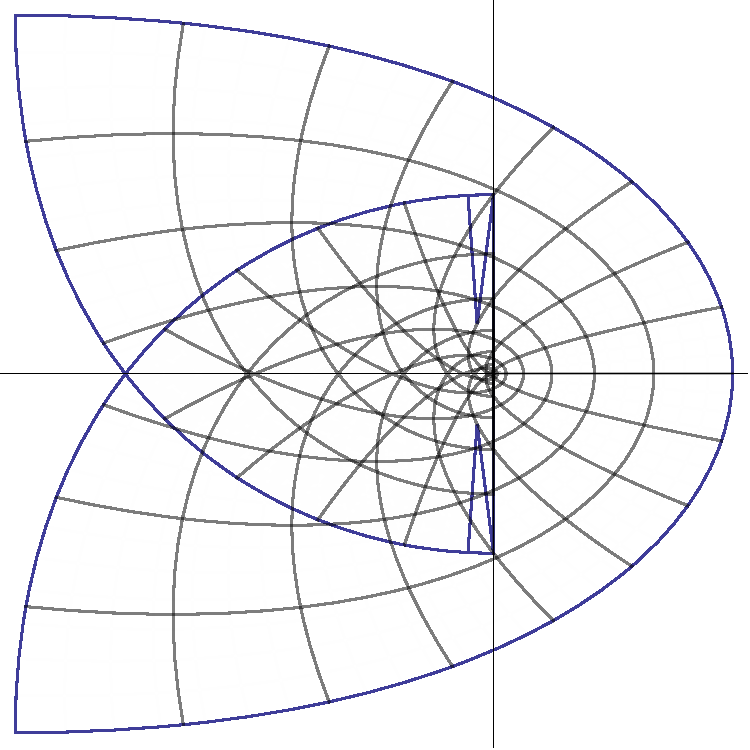
\includegraphics[width=.8\textwidth]{Graphics/conf5.pdf}
  \caption*{$f(z)=z^3$}
  \end{minipage}
  \begin{minipage}{.45\textwidth}
  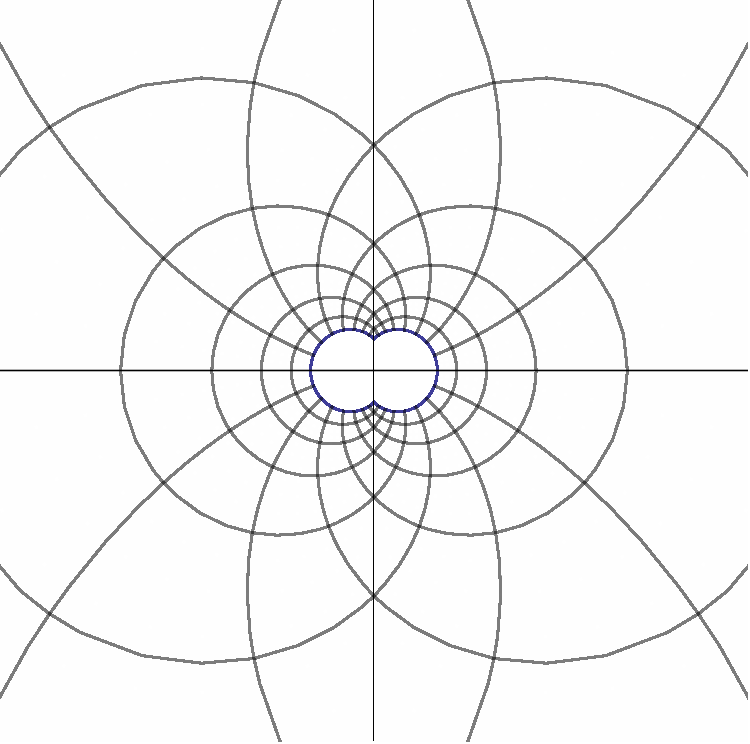
\includegraphics[width=.8\textwidth]{Graphics/conf2.pdf}
  \caption*{$f(z)=1/z^2$}
  \end{minipage}
  
  \bigskip
  \begin{minipage}{.45\textwidth}
  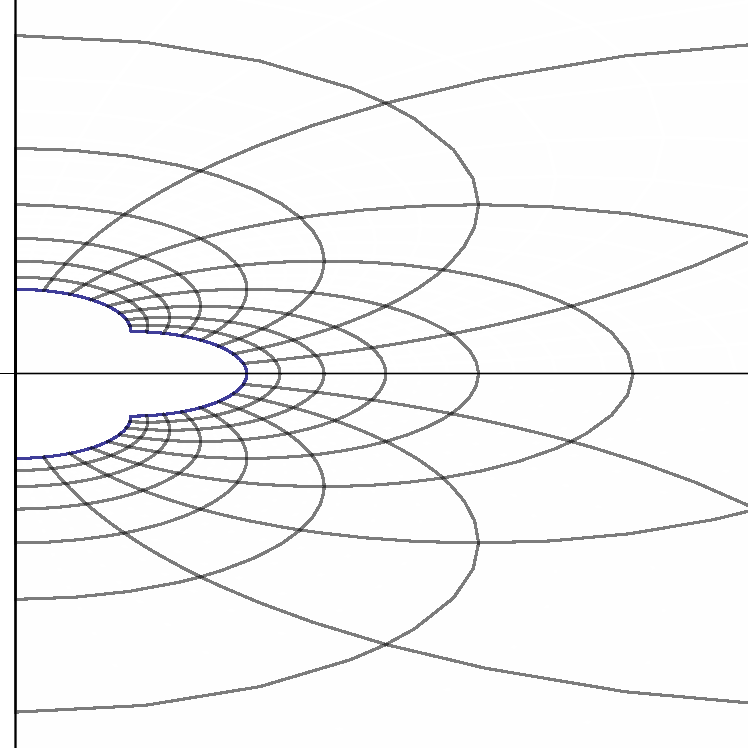
\includegraphics[width=.8\textwidth]{Graphics/conf3.pdf}
  \caption*{$f(z)=1/z$}
  \end{minipage}
  \begin{minipage}{.45\textwidth}
  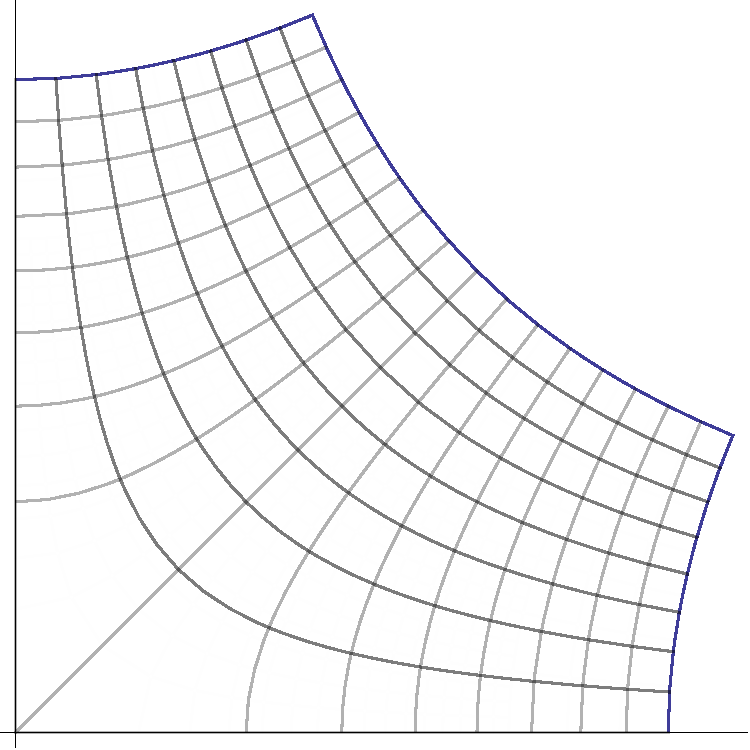
\includegraphics[width=.8\textwidth]{Graphics/conf4.pdf}
  \caption*{$f(z)=\sqrt{z}$}
  \end{minipage}
  \end{figure}
\end{center}
\end{example}
%\pagebreak


%*******************************************************
\section{The Virasoro algebra}
\label{The Virasoro algebra}
Let $\Diff(\s)$ be the group of orientation preserving
diffeomorphisms on $\s$, which in turn coincides with
the conformal transformations leaving the circle invariant. 
Its Lie algebra corresponds to the algebra of smooth
vector fields on the circle whose complexification gives 
rise to the Witt algebra with basis elements $l_n\coloneqq
-z^{n+1} \frac{d}{dz}$, such that
\[
\comm{l_n,l_m}=(n-m)l_{m+n}.
\]
Since we are looking for projective unitary representations of
positive energy we shall be concerned with its unique non-trivial 
central extension (see \cite*{KE:1998}), the Virasoro algebra, 
given in terms of generators $L_n$
\begin{equation}
\label{Vir}
\comm{L_n,L_m}=(n-m)L_{n+m} + \frac{c}{12} m(m^2-1)\,
\delta_{n+m}\bm{1}.
\end{equation}
$L_0$ is referred to as the conformal Hamiltonian and we are interested
in irreducible unitary representations $\pi$ of the above algebra with 
positive energy, namely the spectrum of $L_0$ is required to be positive.
Those representations have been fully classified (see \cite*{FQS})
and are given in terms of pairs $(c,h)$ where $c$ is the central
term appearing in \eqref{Vir} and $h$ is the lowest weight
\[
\pi_{(c,h)}(L_0)\ket{h}=h\ket{h}\qquad \pi_{(c,h)}(L_m)\ket{h}=0,\ m>0.
\]
Positivity of the energy implies $h\geq 0$ and from unitarity it follows
${L_n}^*=L_{-n}$. These conditions give restrictions on the possible
admissible pairs $(c,h)$ and we have that (\cite*{FQS:1984}) either 
$c\geq 1\text{ and }h\geq 0$ or 
\begin{align*}
c=&1-\frac{6}{m(m+1)},\quad m=2,3,\ldots\\ 
\intertext{and}
h=h_{p,q}(c)&=\frac{((m+1)p-mq)^2-1}{4m(m+1)}
\end{align*}
with $p=1,2,\ldots,m-1$ and $q=1,\ldots,p$. Once the lowest weight 
$\ket{h}$ is given the whole representation space (Verma module 
$V(h,c)$) can be obtained as a span of 
\[
\ket{v}=L_{-n_1}\ldots L_{-n_m}\ket{h},\qquad n_1\geq 
\ldots \geq n_m > 0.
\]
The set of vectors obtained with fixed $m$ forms a subspace ${\hil}^m$
of energy $h+(n_1+\ldots +n_m)$. The Hilbert space is then obtained as
completion of the quotient of $\oplus_{m=0}^{\infty}{\hil}^m$ 
with respect to the null vectors \cite*{KE:1998}.



%*******************************************************
\subsection{The M\"obius group}
\label{The Moebius group}
Let us now look at the action of $\textrm{SL}(2,\R)$ on the 
compactified real line $\overline{\R}=\textrm{C}^{-1}(\s)$ by 
\[
x\mapsto gx=\frac{ax+b}{cx+d}\qquad 
g=\begin{pmatrix}
  a&b\\
  c&d
  \end{pmatrix},
\quad \Det g=1.
\]
$\textrm{SL}(2,\R)$ does not act faithfully on $\overline{\R}$
whereas so does its quotient with respect to the kernel 
$\textrm{PSL}(2,\R)\coloneqq \textrm{SL}(2,\R)\mathbin/\set{\pm\bm{1}}$.
We call $\textrm{PSL}(2,\R)$ the M\"obius group and we see it 
can be identified, after Cayley transform, with $\textrm{PSU}(1,1)$ 
acting on the circle as
\[
z\mapsto \frac{\alpha z +\beta}{\bar{\beta}z+\bar{\alpha}}
\qquad 
C(g)=\begin{pmatrix}
  \alpha&\beta\\
  \bar{\beta}&\bar{\alpha}
  \end{pmatrix},
\quad \Det C(g)=1.
\]
Notable one-parameters subgroups are given by rotations, translations and 
dilations, whose action
\begin{align*}
R(\theta)z&=\e^{i\theta}z,\qquad &z\in\s\\
\delta_s x&=\e^s x,\qquad &x\in\R\\
\tau_t x&=x+t,\qquad &x\in\R\\
\end{align*}
is displayed as matrices in $\textrm{PSL}(2,\R)$ as
\[
R(\theta)=\begin{pmatrix}
          \cos\left(\frac{\theta}{2}\right)&\sin\left(\frac{\theta}{2}\right)\\
          -\sin\left(\frac{\theta}{2}\right)&\cos\left(\frac{\theta}{2}\right)
          \end{pmatrix},\quad
\delta_s=\begin{pmatrix}
          \e^{\frac{s}{2}}&0\\
          0&\e^{-\frac{s}{2}} 
          \end{pmatrix},\quad
\tau_t=  \begin{pmatrix}
          1&t\\
          0&1 
          \end{pmatrix}.
\]
A convenient basis for the Lie algebra complexification can be given
in terms of elements $\set{L_0,L_{\pm 1}}$ (see \cite*{Longo:private}) 
satisfying 
\[
\comm{L_1,L_{-1}}=-2 L_0\qquad
\comm{L_0,L_{1}}=-L_{1}\qquad
\comm{L_0,L_{-1}}=L_{-1}
\]
namely they generate the closed subalgebra of \eqref{Vir} with $m,n=0,\pm 1$.
The generators of translations $P$, rotations $K$ and
dilations $D$ can be obtained from
\begin{align*}
L_0&=\frac{1}{2} (P+K)\\
L_{\pm 1}&= \frac{1}{2}(P-K)\pm iD.
\end{align*}
We assume that there
exist a unique vector $\ket{0}$ such that $L_0\ket{0}=L_{\pm 1}\ket{0}=0$
and ergo $U(g)\ket{0}=\ket{0},\,\forall\,g\in \textrm{PSL}(2,\R)$. We call such
a vector the vacuum state and refer to this feature saying that the M\"obius
group is the only subgroup of the conformal transformations on the circle 
preserving the vacuum state. Of course this straightforwardly emerges also
by looking at the explicit realisation of $l_n$ as $-z^{n+1} \frac{d}{dz}$.

\bigskip
The Virasoro algebra generated by the $L_n$ contains many 
copies of the Lie algebra of the cover of the M\"obius group. 
In particular one may define for each $n> 0$
\[
L^{(\pm n)}=\frac{1}{n}L_{\pm n},\quad
L^{(0)}=\frac{1}{n}L_0 +\frac{c}{24}\,\frac{n^2-1}{n}
\]
with commutation relations
\[
\comm{L^{(n)},L^{(-n)}}=2 L^{(0)},\quad
\comm{L^{(\pm n)},L^{(0)}}=\pm L^{(\pm n)}.
\]
The subgroup generated by this sub-Lie algebra  
is isomorphic (\cite{LX:2004}) to
the $n^{\textrm{th}}$ covering of the M\"obius group 
$\textrm{PSU}(1,1)^{(n)}$ acting on $z\in\s$ as
\[
g^{(n)}(z)\coloneqq\sqrt[n]{\frac{\alpha z^n +\beta}
{\conj{\beta}z^n + \conj{\alpha}}}\,.
\]
Equivalently, this group can be defined as the set of all
elements $g\in\Diff(\s)$ for which there exists a M\"obius
transformation $\phi$ such that $g(z)^n=\phi(z^n)$. Clearly,
this is nothing but the definition we just gave above.

As a remark, we shall very often use in the following the
concept on $n$-dilations in the context of modular theory,
where such transformations will be exactly defined as
\[
\delta_t^{(n)}(z)=\sqrt[n]{\delta_t(z^n)}
\]
and thus they appear as standard dilations in 
$\textrm{PSU}(1,1)^{(n)}$. Here $\delta_t$ are 
the single-interval dilations defined as the 
subgroup of the M\"obius group preserving the 
intervals, having the boundaries as fixed points 
(for the precise definition see 
\ref{BW_modular_flow_intervals}).






%*******************************************************
\section{The quarks construction}
\label{The quarks construction}
Let us assume the theory contains many complex fields 
\[
\psi^i(z)=\sum_{s}\psi_s^i\,z^{-s-1/2}
\]
satisfying fermionic anti-commutation relations,
with $(s,r)$ running either in $\Z+1/2$ (vacuum representation) or in
$\Z$ (Ramond representation). Define now the $a^{\textrm{th}}$ current as
(``quark construction'' \cite*{KE:1998}):
\begin{equation}
\label{current}
J^a(z)\coloneqq \frac{1}{2}\,
\sum_{i,j}\,\wick{\,{\psi^*}^i\,\tau^a_{ij}\psi^j\,}(z) 
\end{equation}
where ${\tau}^a\in\mathfrak{g}\subset\mathfrak{u(n)}$ 
is a basis of some matrix Lie algebra. 
The normal ordering $\wick{AB}$ between two operators
is defined by subtraction of the vacuum
expectation value $\wick{AB}\coloneqq AB -\vac(AB)\bm{1}$.
This is a standard definition for observables
in the field theoretical setting in order to avoid
divergences that might otherwise occur when calculating
scattering amplitudes and correlation functions.
As a straightforward consequence of such definition 
the vacuum expectation value of any normal
ordered product vanishes as it is
\[
\vac(\wick{AB})=\vac(AB-\vac(AB)\bm{1})=\vac(AB)
-\vac(AB)=0.
\]
By using the fermionic anticommutation relations one finds that,
expanding in Fourier modes on the circle, $z\in\s$,
\[
J^a(z)=\sum_{n\in\Z} j^a_n\,z^{-n-1},\quad
J^a(x)=-\frac{\dd z}{\dd x}\,J^a(z(x))
\]
and thereby
\begin{equation}
\comm{j^a_n,j^b_m}=f^{ab}_{\phantom{ab}c}\,\j^c_{n+m}
   +n\,\delta_{n+m,0}\,\kappa^{ab}\,k   \label{cur alg modes} 
\end{equation}
Here $f^{ab}_{\phantom{ab}c}$ are the structure constants 
and $k$ is a positive integer, called the ``level'',
that depends on the Lie algebra $\mathfrak{g}$ and
its matrix representation in $\mathfrak{u(n)}$ chosen
for the construction. It characterises the model. 
Furthermore $\kappa^{ab}$ is the Killing form of~$\mathfrak{g}$. 
The latter is the trace of the adjoint
action in the Lie algebra $\ad\colon\mathfrak{g}
\to \textrm{GL}(\mathfrak{g}), x\mapsto\comm{x,\blank}$
\[
\kappa^{ab} = \tr(\ad X^a\circ \ad X^b) 
\]
(see \cite{RehrenERLCFT}, \cite{Fuchs:1992}).
Equation \eqref{cur alg modes} 
defines the non-abelian
current algebra for $\mathfrak{g}\subset \mathfrak{u(n)}$
at level $k$.

\bigskip
In the abelian case the commutation relations for the 
current look $2\pi i\,\comm{j(x),j(y)}=\delta'(x-y)$; the
central operator
\begin{equation}
\label{charge}
Q=\frac{1}{2\pi}\,\int_{\R}\dd x\,j(x)
\end{equation}
is referred to as the ``charge''. In terms of Fourier modes
$j(z)=\sum_{n\in\Z}j_n z^{-n-1}$ the charge 
$Q$ emerges as the mode $j_0$.

\bigskip 
The two-point vacuum correlation function for the current 
can be easily calculated in terms of the fermionic
one by implementing the quark construction. In fact
we have
\[
\vac(j(x)j(y))=\vac(\wick{\psi^*\psi}(x)\,
\wick{\psi^*\psi}(y)).
\]
Standard tools in quantum field theories allow
to work out product of normally ordered operators 
and we remand the reader to any textbook for 
explicit proofs. In particular these are given 
in terms of pairing between operators at 
different points and in the case at hand the
only contractions that matter are
\begin{align*}
\vac(j(x)j(y))&=\vac(\wick{\psi^*\psi}(x)\,
\wick{\psi^*\psi}(y))\\
&=\vac(
\bcontraction{}{\psi(x)^*}{\psi(x)\psi(y)^*}{\psi(y)}
\bcontraction[2ex]{\psi(x)^*}{\psi(x)}{}{\psi(y)^*}
\psi(x)^*\psi(x)\,\psi(y)^*\psi(y))+
\vac(
\bcontraction{}{\psi(x)^*}{\psi(x)}{\psi(y)^*}
\bcontraction[2ex]{\psi(x)^*}{\psi(x)}{\psi(y)}{\psi(y)^*}
\psi(x)^*\psi(x)\,\psi(y)^*\psi(y))\\[2ex]
&=\vac(\psi(x)^*\psi(y))\,\vac(\psi(x)\psi(y)^*)+0\\
&={\vac(\psi(x)^*\psi(y))}^2
\end{align*}
hence once the fermionic two-point function is given,
its square determines $\vac(j(x)j(y))$. However,
the current algebra possesses a continuum of representations
given by the charged states $\omega_q=\vac\circ\rho_q, q\in\R$, 
where $\rho_q$ are automorphisms acting on the currents as
$\rho_q(j(x))=j(x)+2q/(1+x^2)$. The one and two-point functions
are given by
\begin{align*}
\omega_q(j(x))&=\frac{2q}{1+x^2}\\
\omega_q(j(x)j(y))&=\frac{4q^2}{(1+x^2)(1+y^2)}+
\frac{-1}{(x-y)^2}\\
\end{align*}
which read, in terms of the $z$ variable on the circle
\begin{align*}
\omega_q(j(z))&=\frac{q}{z}\\
\omega_q(j(z)j(w))&=\frac{q^2}{wz}+\frac{1}{(w-z)^2}
\end{align*}

\bigskip
Provided the currents, one can construct the ``Sugawara''
stress-energy tensor as
\begin{equation}
\label{SET}
T_S(z)\coloneqq \xi\,\kappa_{ab}\,\wick{\,J^a J^b\,}(z)
\end{equation}
with $\xi$ being a normalisation constant. The
Fourier expansion on the circle reads, in terms of modes,
\[
T_S(z)=\sum_{n\in\Z} L_n\,z^{-n-2}
\]
and thereby the below commutations relations follow
\begin{align}
\comm{L_n,L_m}&=(n-m)L_{n+m} + \frac{c}{12} m(m^2-1)\,
     \delta_{n+m}\bm{1}\notag \\ 
i\,\comm{T(x),T(y)}&=-\left(T(x)+T(y)\right)\delta'(x-y)
     + \frac{c}{24}\delta'''(x-y)\bm{1} \label{LM_cr}
\end{align}
where the central charge $c$ can be expressed as 
(\cite{dFMS:1997}, \cite{Fuchs:1992})
\begin{equation}
\label{coxeter}
c=\frac{k}{k+g}\,\dm\mathfrak{g}
\end{equation}
where $g$ is a group factor determined by group theory (dual
Coxeter number). We have purposely introduced again the 
notation $L_n$ as in
\eqref{Vir} for the Fourier modes of the stress-energy tensor
to explicitely remark that its modes exactly satisfy the
commutation relations defining the Virasoro algebra \eqref{Vir}.
If the theory admits unitary implementations for $z\mapsto g(z)$
then we can write
\[
\alpha_g(\phi(z))=\phi'(g(z))=U(g)\phi(z){U(g)}^*;\quad
U(g)=\e^{iT(f)}
\]
$g(z)$ being $g(z)=\textrm{exp}(f)(z)$.
The zero mode $L_0$ is the conformal Hamiltonian
and it generates the time evolution automorphism
of the current algebra according to
\[
\alpha_t(a)=\e^{itL_0}a\e^{-itL_0}.
\]
The Fermi fields possess by themselves their own 
full stress-energy tensor given by 
\begin{equation}
\label{SET_vac_vs_R}
T_F(z)=\frac{1}{2} \sum_i^N\wick{\,{\psi^*}^i(z)\,
\partial_z\psi^i(z)\,} + \frac{\varepsilon}{16}\,\frac{N}{z^2}
\end{equation}
with $\varepsilon=0,1$ for vacuum representation 
and Ramond representation, respectively. Again, this 
stress-energy satisfies commutation relations of the 
type \eqref{LM_cr}. Nevertheless, in general 
$T_F$ differs from $T_S$; the difference can be computed 
(see \ref{Coset models}) as a new stress-energy tensor
given by $T_F=T_S+T_{\textrm{coset}}$ with central charge 
given by the difference of the two initial central charges:
$c_{\textrm{coset}}=c_F-c_S$. The class of models 
where the difference $T_F-T_S$ happens to be zero are 
referred to as conformal embeddings.




%*******************************************************
\section{Primary fields}
\label{Primary fields}
In the field theoretical setting each vector $\ket{v}\in V(c,h)$  of finite energy
can be thought as $\ket{v} = \lim_{z\to 0} \phi(z) \ket{0},\,\ket{0}$ being
a conformally invariant \emph{vacuum state} (state-field correspondence).
By the spectrum condition (positivity of $L_0$), vector-valued 
distribution on $\s$ as $\phi(z) \ket{0}$ can be analytically continued
to functions in the interior of the circle, so that the limit is
well defined.
\begin{definition}
Fields corresponding to lowest weight vectors $\ket{h}$ are said to 
be primary and of scaling dimension $h$.
\end{definition}
By exploiting the properties of the operators $L_n$ one finds, for 
primary fields, the following commutation relations
\begin{equation}
\label{primary fields}
\comm{L_n,\phi(z)}=h(n+1)z^n\phi(z) + z^{n+1}\partial_z \phi(z)
\end{equation}
which can be exponentiated to
\begin{equation}
\label{finite primary}
\phi(z)=\left(\frac{dg(z)}{dz}\right)^h\phi'(g(z))
\end{equation}
$z\mapsto g(z)$ being any general diffeomorphism of the circle. 
In particular the behaviour of conformally invariant fields
under infinitesimal conformal transformations acquires the 
forms 
\begin{align*}
i\comm{P,\phi(x)}&=\partial_x\phi(x)\\
i\comm{D,\phi(x)}&=(x\partial_x+h)\phi(x)\\
i\comm{K,\phi(x)}&=(x^2\partial_x+2hx)\phi(x)
\end{align*}
which can be derived from \eqref{primary fields} in case
$n=0,\pm 1$. 

\bigskip

Quite often
the theory may also contain further fields, which do not transform
as above because they are obtained out of non-lowest weight vectors.
Such fields, called \emph{secondary} or \emph{descendant}, have 
additional contributions in the transformation laws due to further 
contributions in the commutation relations \eqref{primary fields}.
\begin{example}
The stress-energy tensor defined in \eqref{SET} transforms as
\begin{align*}
T(z)&={\left(\frac{dg(z)}{dz}\right)}^2 T'(g(z)) +
\frac{c}{12} s(g(z),z)\\
\intertext{where}
s(g(z),z)&=\dfrac{d^3 g}{d z^3}/\dfrac{dg}{dz} -\dfrac{3}{2}
{\left(\dfrac{d^2g}{dz^2}/\dfrac{dg}{dz}\right)}^2
\end{align*}
is the Schwarzian derivative. The additional term cancels out if 
$g\in~\textrm{M\"ob}$ (T is \emph{quasi-primary}).
\end{example}
\begin{example}
Fermi fields $\psi(z)$ and currents $J(z)$ are primary fields of
dimensions $1/2$ and $1$, respectively. They therefore transform as
\[
\psi(z)=\sqrt{\frac{dg(z)}{dz}}\,\psi'(g(z))\quad\text{and}\quad
J(z)=\frac{dg(z)}{dz}\,J'(g(z)).
\]
\end{example}


%*******************************************************
\section{Conformal nets}
\label{Conformal nets}
The section at hand deals with some definitions about conformal nets
and their representations in the algebraic setting. For this purpose
let $\mathcal{I}$ be the set of non-empty, non-dense open intervals
on the circle $\s$.
\begin{definition}
A \emph{conformal net} on $\s$ is an assignment of von Neumann algebras
$\I\in \mathcal{I}\to\alg{\I}\subset\bh$ such that the following 
properties hold (\cite*{Ca2004}):
  \begin{enumerate}
   \item \emph{Isotony}:
         \[
         \alg{\I_1}\subset\alg{\I_1}\qquad
         \text{if } \I_1\subset\I_2.
         \]
   \item \emph{Locality}:
         \[
         \alg{\I_1}\subset\alg{\I_2}'\qquad
         \text{if } \I_1\cap\I_2=\emptyset.
         \]
   \item \emph{M\"obius covariance}, namely a strongly continuos unitary 
         representation $U(g)\in\hil$ of the M\"obius group  
         exists such that 
         \[
         U(g)\alg{\I}U(g)^*=\alg{g\,\I}\qquad g\,\in \text{M\"ob}.
         \]
   \item \emph{Positivity of the energy}: $\textrm{spect}\left(U(L_0)\right)
         \geq 0,\,L_0$ being the generator of the one-parameter
         subgroup of rotations $R(\theta)z=\e^{i\theta}z$.
   \item \emph{Existence and uniqueness of the vacuum}:
         \[
         \exists !\ \Omega\in\hil\,\mid
         \textrm{Ker}\left(U(L_n)\right)=\C\Omega.
         \]
         Also, $\Omega$ is assumed to be cyclic, $\ie\ a\Omega$ 
         is dense in $\hil$, and separating, $\ie\
         a_1\Omega=a_2\Omega\Rightarrow a_1=a_2$,
         for the whole algebra $\alg{\s}=\vee_{\I \in\mathcal{I}}
         \alg{\I}$.           
   \end{enumerate}
From the above properties further consequences can be proven, as 
well as:
  \begin{enumerate}[resume]
   \item \emph{Factoriality}: The algebras $\alg{\I}$ are 
         type $\textrm{III}_1$ factors.
   \item \emph{Reeh-Schlieder property}: 
         \[
         \Omega \text{ is cyclic and separating for } 
         \alg{\I},\ \forall\,\I\in\mathcal{I}.
         \]
   \item \emph{Irreducibility}: The von Neumann algebra generated
         by all the intervals exhausts all $\bh$, \ie
         \[
         \underset{\I\in\mathcal{I}}{\bigvee}\alg{\I}=\bh
         \]
   \item \emph{Haag duality}:
         \[
         \alg{\I}'=\alg{\I'}\ \forall\,\I\in\mathcal{I}.
         \]
   \item \emph{Bisognano-Wichmann property}: from Modular Theory it
         follows that the modular operator associated to the pair
         $\left(\alg{\I},\Omega\right)$ is
         \[
         \Delta^{it}_{\left(\I,\Omega\right)}=
         U\left(\Lambda_{\I}^{-2\pi t}\right)
         \]
         where $\Lambda_{\I}$ is the one parameter subgroup of
         M\"ob preserving the interval $\I$ (corresponding to
         the dilations if $C(\I)=\R_+)$.
  \end{enumerate}
\end{definition}
Along the same lines a conformal net is said to be diffeomorphisms
covariant if it admits a strongly continuos projective unitary 
representation $V$ of $\Diff(\s)$ such that
\[
V(h)\alg{\I}{V(h)}^*=\alg{h\,\I}\qquad h\in\Diff(\s).
\]
\begin{definition}[Strong additivity]
The net is said to be \emph{strongly additive} if, for every
pair of intervals $\I_1,\I_2$ obtained by removing a single point
from $\I, \ie\ \I=~\I_1\cup\I_2\cup\set{P}$ we have
\[
\alg{\I_1}\vee\alg{\I_2}=\alg{\I}.
\]
\end{definition}
\begin{definition}[Split property]
The net $\I\to\alg{\I}$ is said to be \emph{split} 
if, for any two intervals $\I, \textrm{J}$ with disjoint
closure, a von Neumann algebras isomorphism
\[
\chi\colon\alg{\I}\vee\alg{\textrm{J}}\to\alg{\I}\otimes
\alg{\textrm{J}}
\]
exists such that $\chi(x y)=x\otimes y,\ 
x\,\in\alg{\I},\,y\,\in\alg{\textrm{J}}$.
Whenever one of the two intervals is contained 
(along with its closure) into the other, say, 
$\overline{\I}\subset\textrm{J}$, this is equivalent 
(\cite*{Longo:private}) to the
existence of an intermediate type I factor $\vN$,
$\alg{\I}\subset\vN\subset\alg{\textrm{J}}$. It is
essential that the two interval neither touch
nor overlap.

\bigskip
The split map is given in terms of a canonical 
unitary between the representing Hilbert spaces 
$V\colon\hil\to\hil\otimes\hil$ such that
\[
V\left(\alg{\I}\vee\alg{\textrm{J}}\right)V^*
=\alg{\I}\otimes\alg{\textrm{J}}
\]
As a consequence  for any given normal states 
$\varphi_i$ on $\alg{\I_i}$ there exists a normal
state $\varphi$ on the total algebra $\vee_{\I}\alg{\I}$ such that
\[
\varphi\left(a_1 a_2\right)=\varphi_1(a_1)\cdot\varphi_2(a_2).
\]
In the language of field theories this property is never fulfilled
by the vacuum state, because splitting the correlation functions
into products would eliminate all correlations between fields
in different points, $\vac(a(x)b(y))\neq \vac(a(x))\cdot\vac(b(y))$.
This means that the state given by $\vac\circ V^*$ onto 
$\alg{\I}\otimes\alg{\textrm{J}}$ is an ``excited state''.

A complete and full characterisation of the split property can 
be found in the literature and we refer the reader to the references. 
In particular it can be shown (\cite*{Longo:private} or \cite*{DLR:2001}) 
that if the conformal Hamiltonian $L_0$ satisfies the trace-class
condition, namely
\[
\tr(\e^{-\beta L_0})<\infty\quad\forall\,\beta>0
\]
then the conformal net is split.
\end{definition}
A \emph{representation} of a conformal net is a family 
$\set{\pi_{\I}}$ where $\pi_{\I}$ is a representation of $\alg{\I}$
on some Hilbert space $\hil_{\pi_{\I}}$ such that
\[
{\pi_{\textrm{J}}\lvert}_{\alg{\I}}=\pi_{\I},\quad \I\subset\textrm{J}.
\]
A unitary equivalence class $[\pi]$ of representations on a separable
Hilbert space is called a \emph{sector}. Since the von Neumann algebras
are by definition subsets of $\bh$ they are already realised on some 
Hilbert space: we refer to their defining representation as to the 
\emph{vacuum sector} of the theory.
Furthermore a representation is said to be M\"obius (diffeomorphisms) 
covariant (\cite*{Ca2004}) if there is a strongly continuous unitary 
representation $U_{\pi}$ of the M\"obius (diffeomorphisms) group such that
\[
U_{\pi}(g)\pi_{\I}\left(\alg{\I}\right){U_{\pi}(g)}^*=
\pi_{g(\I)}\left(\alg{g(\I)}\right)
\]
namely
\[
\ad U_{\pi}(g)\circ\pi_{\I}=\pi_{g(\I)}\circ\ad U(g(\I)). 
\]


\cleardoublepage%************************************************
\chapter{Basics of von Neumann algebras}\label{ch:von Neumann}
\minitoc\mtcskip
%************************************************

\noindent The following sections provide an elementary
introduction to the basic ingredients we shall be dealing 
with, namely operators on Hilbert spaces and von Neumann
algebras (\cite*{Jones:vN}). This is because the main features 
of a physical theory are encoded into the fields content, 
which in turn happen to emerge as operator valued distributions 
assigned to each point of the space-time, $x\mapsto\phi(x)$ 
(\cite*{Haag}). For this reason a systematic analysis of 
their mathematical properties is needed, and tools ought to 
be developed in order to better understand their algebraic 
underlying structure.


%*******************************************************
\section{Basic definitions and operator topologies}
\label{Operator topologies}
Let $\hil$ be a Hilbert space and $\dom{A}\subset\hil$.
An operator on $\hil$ whose domain is $\dom{A}$ is 
a linear map $A\colon\dom{A}\to\hil$.

 \begin{definition}[Operator norm]
 Let $x\in\dom{A}\mid x\neq 0$ and $A\colon x\mapsto A(x)\in\hil$.
 The operator norm of $A$ is defined as
 \begin{equation}
 \label{oper_norm}
 \norm{A}=\sup_{x\in\dom{A}\neq 0}\ 
 \frac{\norm{Ax}}{\norm{x}}.
 \end{equation}
 If $\norm{A}<\infty$ then the operator $A$ is said
 to be bounded.
 \end{definition}
 
 \begin{property}
 An operator $A$ is bounded if and only if it is continuous.
 \end{property}
 
 \begin{property}
 A bounded (and therefore continuous) operator $A$ defined
 on a dense subset $\dom{A}\subset\hil$ can be uniquely extended
 to the whole $\hil$ by continuity.
 \end{property}
 
As a remark we notice that, by continuity, the convergence of
the sequence $x_n\rightarrow x$ in $\dom{A}$ implies the 
convergence of the sequence $A x_n\rightarrow A x$. 

 \begin{definition}[Closed operator]
 Let $x_n\in\dom{A}$ such that $x_n\rightarrow x$. Let us also
 assume that $A x_n\rightarrow y$. The operator $A$ is called
 \emph{closed} if the previous assumptions imply $x\in\dom{A}$ and
 $y=A x$. Equivalently, an operator is closed if its graph is
 closed in the direct sum $\hil\oplus\hil$.
 \end{definition}
 
Take now an operator $A$, not necessarily closed, and assume that
the closure of its graph in $\hil\oplus\hil$ happens to be the graph 
of some operator $\overline{A}$, i.e. if $\overline{G(A)}=G(\overline{A})$.
Then $A$ is said to be ``closable'' and $\overline{A}$ its closure.

 \begin{definition}[Adjoint operator]
 Let $F_x\colon y\in\dom{A}\to\scal{x,Ay}\in\C$ for any operator
 $A$. The set of all points $\set{x\in\hil\mid F_x\text{ is continuous}}$ 
 is defined as $\dom{A^*}$. On this domain, by means of Riesz 
 representation theorem, $\exists !\,z\in\hil\mid F_x(y)=\scal{z,y}$.
 The operator $A^*$ adjoint of $A$ is defined as $A^*x=z$ on $\dom{A^*}$.
 \end{definition}
 
Given any two operators $A$ and $B$ we say that $A\subset B$ if
$\dom{A}\subset\dom{B}$ and $Ax=Bx$ on their common domain, i. e.
$x\in\dom{A}$. A densely defined operator is called \emph{symmetric} 
if $A\subset A^*$ and \emph{self-adjoint} if $A=~A^*$.

\bigskip
Henceforth let $\bh$ denote the set of all bounded operators
on a Hilbert space $\hil$, whose domains then coincide with the 
whole space, that is $\mathfrak{D}=\hil$. We assign the following topologies
on $\bh$ (\cite*{Jones:vN}):
 \begin{definition}[Topologies on $\bh$]
 Let $T_n$ be a sequence of operators and $T$ a ``limit point''
 in $\bh$: 
  \begin{enumerate}
  \item \emph{Norm topology}: $T_n\rightarrow T$ in norm if 
        $\norm{T_n-T}\rightarrow 0$ in the norm topology
        defined above in $\eqref{oper_norm}$.  
  \item \emph{Strong topology}: $T_n\rightarrow T$ strongly
        if $\forall\,x\in\hil$ then $\norm{T_n x- Tx}\rightarrow 0$ 
        in the vector norm of $\hil$.
  \item \emph{Weak topology}: $T_n\rightarrow T$ weakly if $\forall\,
        x,y \in \hil$ then $\scal{T_n x,y}\rightarrow\scal{Tx,y}$
        as complex functionals, i.e. $F_{x,y}(T_n)\rightarrow F_{x,y}(T)$.
  \end{enumerate}
 \end{definition}
 
It is easy to verify that a natural order among these 
topologies exists, namely
\[
\text{ norm topology }\vartriangleright
\text{ strong topology }\vartriangleright
\text{ weak topology}
\]
meaning that if a sequence of operators $T_n$ converges
to $T$ in a topology on the left then it converges
to $T$ in a topology on the right. Stronger topologies
have more open sets than weaker ones, and therefore 
if a set is closed in a weak topology it is also closed
in all the stronger ones.

 \begin{definition}[von Neumann algebra]
 A von Neumann algebra is a subset $\vN\subset\bh$ which is 
 closed under the weak operator topology and contains the
 identity. Its commutant ${\vN}'$ is defined as the set 
 ${\vN}'\coloneqq \set{m'\in\bh\mid \comm{m',m}=0,\ m\in\vN}$
 (similarly for $({\vN}')'={\vN}''$ and so forth).
 \end{definition}
 
 \begin{property}[von Neumann bicommutant theorem]
 Let $\vN={\vN}^*$ be a self-adjoint subalgebra of $\bh$. 
 The following assumptions are equivalent:
  \begin{enumerate}
  \item $\vN={\vN}''$.
  \item $\vN$ is weakly closed.
  \item $\vN$ is strongly closed.
  \end{enumerate}
 \end{property}

%*******************************************************
\section{Classification of factors}
\label{Classification of factors}
 \begin{definition}[Factor]
 The centre of an algebra is the set of all elements
 within that algebra which commute with all the rest,
 that is $Z(\vN)=\vN'\cap\vN$.  
 A von Neumann algebra $\vN$ whose centre is trivial 
 is called a factor, i.e. $Z(\vN)=\C\bm{1}$.
 \end{definition}
 
 \begin{definition}[Projections]
 $p\in\bh$ is called a \emph{projection} if and only if
 $p^2=p=p^*$. Likewise $v\in\bh$ is a \emph{partial isometry}
 if $v^* v=p$ is a projection. Given two projections
 $p$ and $q$, we say they are equivalent ($p\approx q$) 
 if there is a partial  isometry $v$ such that $vv^*=p$
 and $v^* v=q$.
 \end{definition}
 
Given two projections $p,q$ we say that $p\leq q$ if and only
if their ranges are $p\hil\subseteq q\hil$. In addition, a projection
$p$ is said to be minimal if, $\forall\,q\leq p$, either
$q=0$ or $q=p$. Consider now any $q\neq p, q<p$; if there is a partial
isometry $v\in\vN$ such that $v v^*=p$ and $v^* v=q$ then the 
projection $p$ is said to be \emph{infinite} (otherwise $p$
is called \emph{finite}). In a nutshell, then, a finite projection
has no equivalent subprojections, whereas infinite projections
do. Consequently a von Neumann algebra is called infinite if its identity 
is infinite, otherwise it is finite.

\bigskip
 \begin{definition}[Murray-von Neumann classification of factors]
 Projections allow us to classify factors according
 to the following:
  \begin{enumerate}
  \item  A factor $\vN$ with a minimal projection is called a
         Type I factor.
  \item  A factor $\vN$ with no minimal projections but non-zero
         finite projections is called a Type II factor.
  \item  An infinite factor $\vN$ admitting a non-zero linear
         functional (trace) $\tr\colon \vN\to\C$ such that
         
         {\centering
         \begin{enumerate}
          \item $\tr(xy)=\tr(yx)\quad x,y\,\in\vN$,
          \item $\tr(x^* x)\geq 0$,
          \item $\tr$ is ultraweakly continuous,
         \end{enumerate}
         }
         is called a Type $\textrm{II}_1$ factor. The trace is said
         to be normalised if $\tr(\bm{1})=1$.
  \item  A factor of the form $\vN\otimes\bh$, with $\vN$
         Type $\textrm{II}_1$ and $\textrm{dim}\ \hil =\infty$
         is called a Type $\textrm{II}_{\infty}$ factor.
  \item  A factor $\vN$ with no minimal projections, no non-zero
         finite projections is called a Type III factor.
  \end{enumerate}
  \begin{table}[tb]
  \caption{Type of factors}
  \centering
   \begin{tabular}{cp{0.8\textwidth}}
   \toprule
   Type & ``working'' definition\\
   \midrule
   I & with minimal projection; also $\exists\,\hil\mid \vN \cong \bh$.\\[0.5ex]
   II & no minimal projection but non-zero finite projections.\\[0.5ex]
   $\textrm{II}_1$ & infinite factor with no minimal projections
                   and a trace $\tr\colon \vN\to\C$.\\[0.5ex]   
   $\textrm{II}_{\infty}$ & $\vN\otimes\bh,\ \vN$ Type $\textrm{II}_1$
                            and $\textrm{dim}\ \hil =\infty.$\\[0.5ex]                           
   III & the rest, i.e. no minimal projections, no non-zero finite projections.\\
   \bottomrule
   \end{tabular}
  \end{table} 
 \end{definition}

%*******************************************************
\section{Introduction to modular theory}
\label{Introduction to modular theory}
Let $\vN\subset\bh$ be a von Neumann algebra and
$\Omega\in\hil$ a cyclic and separating vector for $\vN$.
The anti-linear operator
\begin{equation}
\label{Tomita}
S_0\colon a\Omega\mapsto a^*\Omega,\quad a\,\in\vN
\end{equation}
is closable (\cite*{BR:1979}) and in general unbounded. 
However, let $S=\overline{S_0}$ be
its closure and $S=J{\Delta}^{1/2}$ the respective polar
decomposition. We call $\Delta$ the modular operator and 
$J$ the modular conjugation associated with the pair
$(\vN,\Omega)$. Via functional calculus the
strongly continuous unitary group 
\[
\Delta^{it}=\e^{it \ln\Delta},\quad t\in\R
\]
may be defined and its adjoint action
\begin{equation}
\label{modular group}
\sigma^t_{(\vN,\Omega)}(m)\coloneqq \Delta^{it}\,m\,\Delta^{-it},
\quad m\,\in\vN,\ t\,\in\R
\end{equation}
induces a one-parameter automorphisms group of $\vN$ called
the \emph{modular automorphisms group}. 
A fundamental result in this respect is the

 \begin{theorem}[Tomita-Takesaki (\cite*{BR:1979})]
 Under the previous assumptions the following statements hold:
 the operator $J=J^*$ is anti-unitary and
  \begin{gather}
  J\vN J={\vN}'\\
  \sigma^t_{(\vN,\Omega)}(\vN)=\vN,\quad \forall\,t\,\in\R.
  \end{gather}
 \end{theorem}
The algebra is sent into its commutant by the adjoint action of the
modular conjugation $J$ and the modular group acting of $\vN$
exhausts all the algebra itself. Since all these quantities
explicitly depend on the pair $(\vN,\Omega)$ we have different
realisations of the modular automorphism group according to this choice. 
The characterisation of its shape, according to the choices 
of $(\vN,\Omega)$ in some particular cases, is the main topic 
of the work at hand.

 \bigskip
 The trivial case, i.e. when the algebra is commutative, is very
 easy to handle; take $a,b\,\in\vN$ and look at 
 $\scal{S\,a\Omega,S\,b\Omega}$, with $S$ defined as \eqref{Tomita}:
 \begin{align*}
 \scal{S\,a\Omega,S\,b\Omega}&=\scal{a^*\Omega,b^*\Omega}\\
 &=\scal{\Omega, ab^*\Omega}\\
 \intertext{by commutativity it follows then}
 &=\scal{\Omega, b^*a\Omega}=\scal{b\Omega, a\Omega}\\
 &=\overline{\scal{a\Omega,b\Omega}}
 \end{align*}
 therefore $S$ is antiunitary and hence $\Delta=\abs{S}=\bm{1}$.
 This implies that the action of the modular group
 is trivial on each element of the algebra.


 
 \subsection{\acf{KMS} condition}
 \label{KMS}
 Let $\vN$ be a von Neumann algebra and $\varphi$ a faithful normal
 state on $\vN$. Let furthermore $\sigma_t$ be a weakly
 continuous one-parameter group of automorphisms of $\vN$. 
 Fixed $a,b\,\in\vN$ consider $F_{a,b}(t)\coloneqq
 \varphi(a\,\sigma_t(b))$ as a function in the variable $t\,\in\R$.
 The state $\varphi$ is said to satisfy the Kubo-Martin-Schwinger
 (\ac{KMS}) condition at inverse temperature $T=\beta^{-1},\,0<\beta
 <\infty$ if 
 \begin{enumerate}
  \item $F_{a,b}(t)$ can be analytically continued in 
        the strip $0< \im{t}<\beta$. It is continuous at 
        the boundaries $\im{t}=0,\beta$ and
  \item $F_{a,b}(t+i\beta)=\varphi(\sigma_t(b)a)$.
 \end{enumerate}
 Notice that if the algebra were commutative then every state would
 satisfy the \ac{KMS} condition at $\beta=0$, by commutativity. 
 If this only happens as a special feature of the state at hand then
 $\varphi$ is said to be \emph{tracial}, otherwise $\beta\neq 0$ 
 measures the deviation of $\varphi$ from being a trace. Next note
 that a state is \ac{KMS} with respect to $\sigma_t$ at 
 $T^{-1}=\beta\neq 0$  if and only if it is \ac{KMS} with respect 
 to $\sigma_{-\beta t}$ at $T=-1$; therefore
 by rescaling the group parameter one can always refer to state
 of temperature $-1$. Albeit we shall not discuss this issue
 any further, \ac{KMS} states characterise equilibrium states in
 quantum thermodynamics where the one-parameter group $\sigma_t$
 plays the role of a given time evolution; however, to whom it may
 concern, a full characterisation and a systematic study of
 \ac{KMS} states is provided in \cite*{BRII:19781}.

 \medskip
 The remarkable connection with modular theory is that a normal
 state happens to be a \ac{KMS} state with respect to its own modular 
 group (\cite*{Haag}); the converse is also true, namely the modular 
 group is the only one-parameter group of inner
 automorphisms satisfying the \ac{KMS} condition on the state where it
 comes from. This feature will be fully used in the following to
 characterise and investigate properties of the modular group
 related to different states and algebras.
 
 
 
 \subsection{Bisognano-Wichmann property}
 \label{BiWi}
 As a matter of example let us consider a very important result obtained 
 by Bisognano and Wichmann (\cite*{BiWi:1975}), and so far the only (up to
 geometric transformations) explicit characterisation of modular operators
 for space-time regions.
 
 \medskip
 Let $\wed_{R,L}\coloneqq \set{x\in {\vN}^4\mid x^1\gtrless
 \abs{x^0}}$ be the right (left) wedge region as a subset of the space-time
 $\vN^4$. There is exaclty a one-parameter subgroup of the Lorentz
 group preserving the wedge, namely mapping the wedge into itself:
 \begin{equation}
 \label{Lor_boost}
 \Lambda(t)= \begin{pmatrix}
             \cosh(t)& -\sinh(t) & 0 & 0\\
             -\sinh(t)&\cosh(t) & 0 & 0\\
             0 & 0 & 1 & 0\\
             0 & 0 & 0 &1             
             \end{pmatrix}.
 \end{equation}
 Let the local von Neumann algebra $\alg{\wed}$ be generated by 
 Wightmann fields $W(f)$ and let us choose as a cyclic and separating vector
 the vacuum $\Omega$ as \ac{GNS} of $\vac\left(W(f)\right)=\e^{-1/2{\norm{f}}^2}$. 
 The modular group associated to the pair $\left(\alg{\wed},\Omega\right)$
 coincides with the unitary representation of the subgroup preserving
 the wedge and the modular conjugation acts as reflection through the edge
 of the wedge, changing sign to both $x^0$ and $x^1$
 \begin{equation}
 \label{BiWi}
 \Delta^{it}=U(\Lambda_{\wed}(-2\pi t))\qquad
 J=U(r_{\wed}).
 \end{equation}
 However, since the vacuum is invariant under Poincar\'{e}
 transformations $g$, this result can be generalised to any
 region of the form $\wed'= g\wed $. Setting
 (\cite*{Longo:private})
 \[
 \Lambda_{{\wed}'}(t)=g\,\Lambda_{\wed}\,g^{-1}
 \qquad
 r_{{\wed}'}=g\,r_{\wed}\,g^{-1} 
 \]
 we obtain (\cite*{Guido:2011} and \cite*{GLW:1998})
 \[
 \Delta^{it}=U(\Lambda_{\wed'}(-2\pi t))\qquad
 J=U(r_{\wed'}).
 \]
 It can be shown (again \cite*{Guido:2011}) that the 
 Bisognano-Wichmann property also holds for conformally 
 covariant theories that split into tensor products of 
 two nets on a line, as described in \ref{Conformal nets}. 
 In fact, in two dimensions a wedge reduces to the cartesian 
 product of two half-lines $\R_+\times\R_-$. In the particular
 case where $\I=\R^+$ the modular group explicitly acts as dilations
 with a scaling factor of $\e^{-2\pi t}$
 \[
 \sigma_t\blank=\delta_{\lambda_t}\blank,
 \qquad \lambda_t=\e^{-2\pi t}
 \]
 The two-dimensional modular flow is then $\delta_{\lambda_t}
 \otimes\delta_{\lambda^{-1}_t}$. Intervals can be obtained 
 as conformal transformations of the real line and hence 
 in this case the modular group, corresponding to the 
 subgroup of the Lorentz transformations preserving the wedge, 
 is replaced by the subgroup of the M\"obius transformations 
 fixing each interval, either on the circle picture $\s$ or 
 on the real line.
 
 \begin{minipage}{.35\textwidth}
 \centering 
 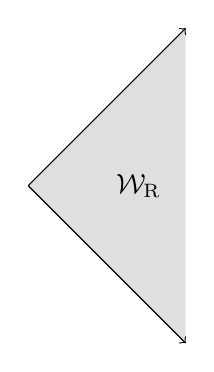
\begin{tikzpicture}[scale=2]
 \fill[gray!25] (0,0)--(1,1)--(1,-1);
 \draw [->] (0,0) -- (1,1);
 \draw [->] (0,0) -- (1,-1); 
 \node at (0.7,0) {$\wed_{\textrm{R}}$};
 \end{tikzpicture}
 \end{minipage}
 \qquad
 \begin{minipage}{.60\textwidth}
 \begin{tikzpicture}[scale=2]
 \draw [->] (0,0) -- (1,1);
 \node [rotate around={45:(-1.5,3)}] {\footnotesize $\R_+$};
 \node at (1.27,0.5) {$\bigtimes$};
 \draw [->] (1.5,1) -- (2.5,0);
 \node [rotate around={-45:(2.9,-5.8)}] {\footnotesize $\R_-$};
 \end{tikzpicture}
 \end{minipage} 
 
 \medskip
 As already mentioned above, the modular group $\sigma^t_{\Omega}$ 
 uniquely satisfies  the \ac{KMS} condition on $\Omega$ and hence
 it characterises thermal equilibrium states for an observer whose
 dynamics is given by $\sigma^t_{\Omega}$. According to this 
 interpretation, the Bisognano-Wichmann property for wedge regions 
 states that the vacuum state is a thermal equilibrium state with 
 temperature $T=-1$ for an observer accelerated with Lorentz boosts.
 This is the case for an observer moving around the event horizon
 of a black hole and the example provides an explanation of the
 Unruh effect, by which the vacuum state
 behaves like a thermal states for observers moving in a 
 gravitational field (\cite{ConRov:1994, MartRov:2003}). 
 In fact, the trajectory of an observer moving in such 
 an event horizon (corresponding in turn to a wedge region) 
 with constant acceleration $a$ is given by the orbits of the 
 Lorentz boosts of the form \eqref{Lor_boost} with the 
 proper ``physical'' time $\tau$ being $t/a$. 
 Therefore the trajectory in the wedge can be
 parametrised as 
 \[
 x^{\mu}(\tau)=1/a\,(\sinh(a\tau),\cosh(a\tau),0,0)
 \]
 and the evolution at later times is $x(\tau_0+\tau)=
 \Lambda(a\tau)x(\tau_0)$. On the other hand, as we 
 have seen in equation \eqref{BiWi}, the modular group 
 with respect to the vacuum state act as a Lorentz boost
 of parameter $-2\pi s$ and satisfies the \ac{KMS} 
 property. Therefore, by uniqueness, the relation between
 the physical time $\tau$ and the modular parameter $s$
 has to be $-2\pi s=a\tau$, in order to give back 
 the Unruh inverse temperature $\beta=-\dd \tau/\dd s=2\pi/a$.
 
 \subsection{Reconstruction of the translations}
 \label{Reconstruction of the translations}
 As just stated, the modular group associated with the pair
 $(\alg{\mathcal{W}},\Omega)$, $\mathcal{W}$ being a wedge region,
 acts like the associated group of Lorentz boosts and this 
 preserves the wedge itself. Remarkable results by Borchers 
 \cite*{Borch:1992} and Wiesbrock \cite*{Wies1,Wies2,Wies3}
 showed that it is possible, under suitable conditions, to
 recover the translations group out of modular data.
 
 \begin{definition}
 Let $\vN$ be a von Neumann algebra with a cyclic and separating
 vector $\Omega$. Let furthermore $U(a)\coloneqq \e^{iaH},\,a\in\R$, 
 be a continuous one-parameter group of unitaries with positive
 generator $H$ leaving $\Omega$ invariant, i. e. $U(a)\Omega=
 \Omega$. The triple $(\vN, H\geq 0, \Omega)$ is called a 
 ``Borchers triple''. Also, the triple is said to satisfy the 
 \emph{half-sided translations} condition if
 $\ad{U(a)}\vN\subset\vN,\ a>0$. 
 \end{definition}
 \begin{theorem}[\cite*{Borch:1992}]
 \label{Borchers}
 Let $\vN$ be a von Neumann algebra with a cyclic and separating
 vector $\Omega$ and denote as $\Delta, J$ the modular data of the pair
 $(\vN,\Omega)$. Then, given a half-sided translated Borchers 
 triple as above, the following  holds
 \begin{align}
 \Delta^{it}U(a)\Delta^{-it}&=U(\e^{-2\pi t}a)\label{Bor}\\
 JU(a)J&=U(-a), 
 \end{align}
 namely $U(a)$ is seen to satisfy translations-dilations commutation relations
 with~$\Delta^{it}$.
 \end{theorem}
 A stronger result provided by Wiesbrock holds true: given two algebras
 in suitable position one can automatically recover the unitaries
 $U(a)$ out of their modular operators only; the construction is showed
 below.
 \begin{definition}
 Let $\mathcal{N}\subset\vN$ be two von Neumann algebras with common
 cyclic and separating vector $\Omega$ and denote with $\Delta_{\vN},
 \Delta_{\mathcal{N}}$ the respective modular operators. We call the 
 inclusion $\mathcal{N}\subset\vN$ half-sided modular (\cite*{Wies1})
 if $\Delta_{\vN}^{-it}\mathcal{N}\Delta_{\vN}^{it}\subset\mathcal{N}$
 for $t\geq 0$.
 \end{definition}
 \begin{theorem}[\cite*{Wies1}]
 \label{Wies:th}
 Under the previous assumptions of half-sided modular inclusion
 $\mathcal{N}\subset\vN$ let $H\coloneqq 1/2\pi 
 \left(\ln \Delta_{\mathcal{N}}-\ln \Delta_{\vN}\right)$; 
 the triple $(\vN, H\geq 0, \Omega)$ is a half-sided translated
 Borchers triple fulfilling theorem \ref{Borchers}. 
 \end{theorem}
 This result suggests that the information about the translations
 is contained into the mutual positions of the two algebras and their
 common cyclic and separating vector. As an important application
 of such result we mention that wedge regions and their translated
 indeed satisfy the half-side modular inclusions and therefore
 the above results directly apply. Representations of the 
 Lorentz boosts emerge as modular operator $\Delta^{it}_{\vN}$ (as a 
 consequence of the Bisognano-Wichmann property) and  
 translations may be recovered by means of the Wiesbrock procedure
 (in two dimensions these exhaust the whole Poincar\'{e} group).
 

 

 
 

 
 

\cleardoublepage
\epigraph{In AQFT it is a long outstanding question,
	     what physical meaning the Tomita-Takesaki
            modular objects have.}%
           {H.-W. Wiesbrock, \emph{Commun.\ Math.\ Phys.\  
           {\bf 157}, 83 (1993)}.}
\part{Multi-geometric modular action in quantum
     field theory}
\cleardoublepage%************************************************
\chapter{Multi-geometric modular theory}
         \label{ch:multi-geometric}
\minitoc\mtcskip
%************************************************

%*******************************************************
 \section{Representations of Fermi fields on the circle}
 \label{repn of Fermi on the circle}
 We are now interested in the positive energy representation
 of real Fermi fields in one dimension, namely fields localised
 on the real line (or similarly on the circle via Cayley
 transform) such that $\psi(x)^*=\psi(x)$ which satisfy 
 anti-commutation relations as distribution in the form
 \[
 \ant{\psi(x),\psi(y)}=\delta(x-y),\quad x,y\,\in\R.
 \]
 In terms of the compact picture the equation takes the
 form
 \[
 \ant{\psi(z),\psi(w)}=2\pi iz\,\delta(z-w)\quad z,w\,\in\s
 \]
 and consequently fields are meant to be smeared with
 functions $f\in\LL{\s}$. In one dimension, as easily seen,
 locality is ensured by disjointness. We recall that by means
 of the anti-commutators
 \eqref{CAR} Fermi fields are bounded operators because 
 $\psi(f)\psi(f)^*+\psi(f)^*\psi(f)=\norm{f}^2_{\hil}\cdot 
 \bm{1}$.
 
 \bigskip
 By using the \ac{GNS} construction, representations can arise
 after choosing appropriate states on the algebra of fields. In
 particular, we shall look at quasi-free states, namely
 states whose high order correlations functions can be
 calculated by using Wick theorem (\cite{BR:1979} and
 \eqref{wick}) as combinations of two-point functions. 
 Therefore the only ingredient we need is the assignment 
 of $\varphi(\psi(x)\psi(y))$.
 
 The vacuum representation of real Fermi fields
 in one dimension emerges out of the vacuum two-point
 function that we already calculated in the
 example \eqref{vacuum2}
 \begin{equation*}
 \vac(\psi(x)\psi(y))=\lim_{\varepsilon\searrow 0}
 \frac{-i}{x-y-i\varepsilon}.
 \end{equation*}
 This gives back, via \ac{GNS} construction, the vacuum 
 representation $\pi_0(\psi(x))$. Using the Cayley
 transform and the standard transformation laws for fields
 \[
 x\mapsto z=\frac{1+ix}{1-ix},\quad
 \psi(z)=\sqrt{-i\,\frac{dz}{dx}}\,\psi(x)=
 \frac{1-ix}{\sqrt{2}}\,\psi(x)
 \]
 we obtain the periodic representation (Neveu-Schwarz) 
 of fields on the circle given
 in terms of Fourier modes as
\[
\pi_0\left(\psi(z)\right)=\sum_{r\in\Z+1/2}\psi_r\,
z^{-r-1/2}\,
\]
 with two-point function $\vac(\psi(z)\psi(w))=
 \displaystyle{\lim_{\lambda\nearrow 1} \frac{1}{z-\lambda w}}$.
  
 \bigskip
 Taking two copies of real Fermi field we obtain a
 representation for the complex Fermi field 
 $\phi(x)=\left(\psi_1(x)+i\psi_2(x)\right)/\sqrt{2}$
 with anti-commutation relations given by
 \[
 \ant{\phi(x),\phi(y)^*}=\ant{\phi(x)^*,\phi(y)}=
 \delta(x-y)
 \]
 and vacuum two-point function 
 \[
 \vac(\phi(x)\phi(y)^*)=
 \vac(\phi(x)^*\phi(y))=\vac(\psi(x)\psi(y)).
 \]
 On the cirle instead the adjoint relation reads 
 $\phi(z)^*=z\,\phi^{\dagger}(z)$
 and the two-point function becomes again $\vac(\phi(z)\phi(w)^*)=
 \vac(\phi(z)^*\phi(w))=\vac(\psi(z)\psi(w))$. 
 
 \bigskip
 Notice that the vacuum state is invariant under the action
 of M\"obius transformations of the form described in
 \ref{The Moebius group}, $\vac\circ \alpha_g=\vac$, where 
 $g\in\textrm{PSL}(2,\R)= \textrm{SL}(2,\R)\mathbin/\set{\pm\bm{1}}$ 
 and $\alpha_g$ is its implementation on the algebras as
 \[
 \alpha_g(\psi(x))=\sqrt{\frac{dg}{dx}}\,\psi(g(x)).
 \]
 Consequently, the vacuum representation is covariant.
 
 \bigskip
 Another positive energy representation can be constructed
 out of the Ramond two-point function
 \begin{equation}
 \label{Ramond}
 \omega_{\textrm{R}}(\psi(x)\psi(y))=
 \lim_{\varepsilon\to 0}\frac{1+xy}{\sqrt{1+x^2}\sqrt{1+y^2}}
 \cdot\frac{-i}{x-y-i\varepsilon}
 \end{equation}
 whose expression in the compact picture is
 \[
 \omega_{\textrm{R}}(\psi(z)\psi(w))=\lim_{\lambda\nearrow 1}
 \frac{z+w}{2\sqrt{zw}}\cdot\frac{1}{z-\lambda w}\,.
 \]
 This gives rise to the Ramond representation in terms
 of Fourier modes as
 \[
 \ram{z}=\sum_{n\in\Z}\psi_n \,z^{-n-1/2}
 \]
 which extends anti-periodically on the circle. This 
 reflects the fact that only local observables, such
 as currents as bilinear forms in the fields, need 
 to be well defined after rotations of $2\pi$ on the
 circle, but Fermi fields themselves need not to.
 
 
 \section{Operator product expansions}
 \label{OPE}
 Let us consider the positive energy representations
 for Fermi fields on the circle as described in the 
 previous paragraph
 \begin{align*}
 \pi_0\left(\psi(z)\right)&=\sum_{r\in\Z+1/2}\psi_r\,
 z^{-r-1/2}\\[2ex]
 \pi_{\textrm{R}}(\psi(z))&=\sum_{n\in\Z}\psi_n \,z^{-n-1/2}
 \end{align*}
 the former being periodic after rotations of $2\pi i$,
 the latter being anti-periodic
 \begin{align*}
 \pi_0\left(\psi(\e^{2\pi i} z)\right)&=\pi_0\left(\psi(z)\right)\\
 \pi_{\textrm{R}}(\psi(\e^{2\pi i}z))&=-\pi_{\textrm{R}}(\psi(z)).
 \end{align*}
 Either of these boundary conditions ensure the correct
 commutation relations between currents once one
 performs the quarks construction. So to speak, only
 local observables, as the currents are, must be well
 defined, but Fermi fields themselves are allowed to carry
 an additional minus sign without affecting the
 algebraic relations. For the sake of notations we may
 write either representations as \cite{Fuchs:1992}
 \[
 \psi(z)=\sum_{s}\psi_s\,z^{-s-1/2}
 \]
 and intend $s\in\Z+1/2$ and $s\in\Z$ for the vacuum
 and Ramond representation, respectively. Anti-commutation 
 relations between Fourier modes can be written as
 \[
 \ant{\psi_s,\psi_t}=\delta_{s+t,0}
 \]
 and the modes themselves can be expressed as
 \[
 \psi_s =\frac{1}{2\pi i}\oint\dd z\,z^{-s-1/2}
 \,\psi(z).
 \]
 With the help of the above relation we can write the 
 anti-commutator between fields in terms of the 
 analogue between modes through
 \[
 \ant{\psi(z),\psi(w)}=\frac{1}{\sqrt{zw}}\sum_{s,r}
 z^{-s}\,w^{-r}\ant{\psi_s,\psi_r}.
 \]
 Such an expression may, in principle, be worked out
 making use of the delta function to help the summation:
 $\ant{\psi_s,\psi_t}=\delta_{s+t,0}$ gives
 \begin{equation*}
 \ant{\psi(z),\psi(w)}=\frac{1}{\sqrt{zw}}
 \sum_{r}{\left(\frac{w}{z}\right)}^r=
 \frac{1}{\sqrt{zw}}\left(
 \sum_{r\geq 0}{\left(\frac{w}{z}\right)}^r+
 \sum_{r<0}{\left(\frac{w}{z}\right)}^r
 \right);
 \end{equation*}
 at a first glance problems occur because, although we
 can split the summation into two contributions, each
 of them represents a geometric series whose domain
 of convergency depends on the particular choice
 of the variables $z,w$. In particular the former
 term converges for $\abs{z}>\abs{w}$, the latter
 otherwise, namely $\abs{z}<\abs{w}$. This means that,
 in order to make sense, we must introduce in the above
 equation particular prescriptions on the choice of the
 allowed variable. To do so we shall proceed as follows:
 we invert back such formula to have
 \[
 \ant{\psi_s,\psi_t}=\frac{1}{2\pi i}\oint \dd z\,
 \frac{1}{2\pi i}\oint \dd w\,z^{s-1/2}\,w^{t-1/2}\,
 \ant{\psi(z),\psi(w)}
 \]
 and consider, on the right hand side, only those
 contours of integrations where each single term
 in the anti-commutator is radially ordered:
 $\ant{\psi(z),\psi(w)}=\psi(z)\psi(w)|_{\abs{z}>\abs{w}}
 +\psi(w)\psi(z)|_{\abs{z}<\abs{w}}$. 
 
 \begin{figure}[htbp]
 \centering
 \def\first{0.5}
 \def\second{0.9}
 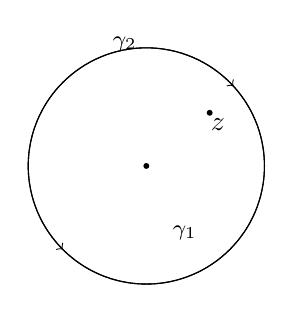
\begin{tikzpicture}[scale=1.5]
 % circle
 \path (0,0) coordinate (O);
 \draw [fill] (O) circle [radius=0.02];
 \draw [decoration={markings, mark=at position 0.625 with {\arrow{>}}},
        postaction={decorate}](O) circle (\first);
 \draw [decoration={markings, mark=at position 0.125 with {\arrow{<}}},
        postaction={decorate}](O) circle (\second);
 \draw [fill] (40:0.7) circle [radius=0.02];
 \node at (30:0.7) {$z$};
 \node at (300:0.65) {\footnotesize$\gamma_1$};
 \node at (100:1.05) {\footnotesize$\gamma_2$};
 \end{tikzpicture}
 \end{figure}
 Once we fix the variable $z\in\C$ the integration
 contours for $w$ must be chosen as $\gamma_1$ 
 to ensure $\abs{z}>\abs{w}$ and as $\gamma_2$ 
 to ensure the converse. The anti-commutator between
 the modes becomes then
 \begin{multline*}
 \ant{\psi_s,\psi_t}=\frac{1}{2\pi i}\oint_0 \dd z
 \left(\frac{1}{2\pi i}\oint_{\gamma_1} \dd w
 \,z^{s-1/2}\,w^{t-1/2}\,\psi(z)\psi(w)\right.\\
 \left.+\oint_{\gamma_2} \dd w
 \,z^{s-1/2}\,w^{t-1/2}\,\psi(w)\psi(z)\right).
 \end{multline*}
 We define the operator product expansion of two Fermi
 fields as
 \[
 \OPE\left(\psi(z)\psi(w)\right)\coloneqq
 \begin{cases}
 \psi(z)\psi(w)&\mbox{ if }\abs{z}>\abs{w}\\
 -\psi(w)\psi(z)&\mbox{ if }\abs{z}<\abs{w}
 \end{cases}
 \]
 and with the help of this definition the integral
 can be rewritten as
 \[
 \ant{\psi_s,\psi_t}=\frac{1}{2\pi i}\oint_0 \dd z\,
 \frac{1}{2\pi i}\oint_{\gamma_1 \cup\gamma_2} \dd w\,
 z^{s-1/2}\,w^{t-1/2}\,\OPE\left(\psi(z)\psi(w)\right).
 \]
 \begin{figure}[htbp]
 \begin{minipage}{0.5\textwidth}
 \centering
 \def\first{0.5}
 \def\second{0.9}
 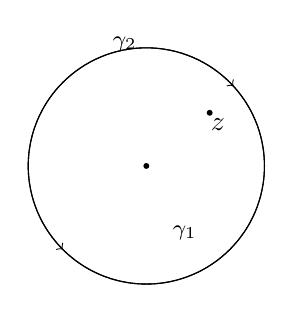
\begin{tikzpicture}[scale=1.5]
 % circle
 \path (0,0) coordinate (O);
 \draw [fill] (O) circle [radius=0.02];
 \draw [decoration={markings, mark=at position 0.625 with {\arrow{>}}},
        postaction={decorate}](O) circle (\first);
 \draw [decoration={markings, mark=at position 0.125 with {\arrow{<}}},
        postaction={decorate}](O) circle (\second);
 \draw [fill] (40:0.7) circle [radius=0.02];
 \node at (30:0.7) {$z$};
 \node at (300:0.65) {\footnotesize$\gamma_1$};
 \node at (100:1.05) {\footnotesize$\gamma_2$};
 \end{tikzpicture} 
 \end{minipage}
 %%%%%%%%%%%%%%
 \begin{minipage}{0.5\textwidth}
 \centering
 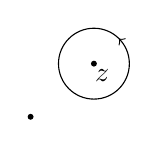
\begin{tikzpicture}[scale=1.5]
 % circle
 \path (0,0) coordinate (O);
 \draw [fill] (O) circle [radius=0.02];
 \draw [fill] (40:0.7) circle [radius=0.02];
 \node at (30:0.7) {$z$};
 % circle around z
 \draw  [decoration={markings, mark=at position 0.125 with {\arrow{>}}},
        postaction={decorate}] (40:0.7) circle [radius=0.3];
 \end{tikzpicture} 
 \end{minipage}
 \end{figure} 
 
 It is even easier if we consider that $\gamma_1\cup
 \gamma_2$ can be shrinked down to a loop around the
 point $z$ so that the integral becomes
 \[
 \ant{\psi_s,\psi_t}=\frac{1}{2\pi i}\oint_0 \dd z\,
 \frac{1}{2\pi i}\oint_z \dd w\,
 z^{s-1/2}\,w^{t-1/2}\,\OPE\left(\psi(z)\psi(w)\right).
 \]
 It is now pretty clear that if no divergences occur
 in the $\OPE$ then, by means of the Cauchy theorem, the 
 integral on the right hand side vanishes. Therefore poles must
 occur in order to have reasonable anti-commutators. 
 In general we can assume that fields in the operator 
 product expansions
 are everywhere analytic except at coinciding points
 $z=w$ and hence the prototype expansion would have
 the form of a Laurent series (\cite{Fuchs:1992})
 \begin{equation}
 \OPE\left(A(z)B(w)\right)=\sum_{n=-n_0}^{\infty}
 c_n(w)(z-w)^n
 \end{equation}
 where the divergences occur for negative $n$ and all 
 the other regular terms, althoug present in the expansion,
 give no actual contribution to the integrals, nor 
 do they to correlation functions. The singular terms
 in the expansion are referred to as the ``contractions'' 
 of the operators and the coefficient $c_0$ is the ``normal
 ordered product''
 \[
 \bcontraction{}{A(z)}{}{B(w)}A(z)B(w)\coloneqq
 \sum_{n=-n_0}^{-1}c_n(w)(z-w)^n,\qquad
 \wick{A(z)B(z)}\coloneqq c_0(z)
 \]
 so that the $\OPE$ is decomposed into
 \[
 \OPE\left(A(z)B(w)\right)=
 \bcontraction{}{A(z)}{}{B(w)}A(z)B(w)+
 \wick{A(z)B(z)}+
 \text{regular terms}.
 \]
 No regular terms occur for free fields, therefore we shall 
 very often omit them, since we are only dealing with 
 such models.
 The number $n_0$ and the actual form of the expansion
 depend upon the fields and the commutation relations
 we want to realise. In the following two explicit examples 
 of $\OPE$, for Fermi fields and for currents, will reproduce
 the standard algebras we are used to.
 
 \begin{example}[$\OPE$ for Fermi fields]
 The operator product expansion for fermions acquires the
 form
 \begin{equation}
 \label{OPEfermions}
 \OPE\left(\psi(z)\psi(w)\right)=
 \begin{cases}
 -\dfrac{1}{z-w}&\mbox{ vacuum rep'n}\\
 -\dfrac{1}{z-w}\cdot\dfrac{1}{2}\left(\sqrt{\dfrac{z}{w}}\right.
 \left. +\sqrt{\dfrac{w}{z}}\right)&\mbox{ Ramond rep'n}
 \end{cases}
 \end{equation}
 which can be proven right by reproducing the correct 
 relations for the anti-commutators. In fact, substituting back into
 \[
 \ant{\psi_s,\psi_t}=\frac{1}{2\pi i}\oint_0 \dd z\,
 \frac{1}{2\pi i}\oint_{z} \dd w\,
 z^{s-1/2}\,w^{t-1/2}\,\OPE\left(\psi(z)\psi(w)\right).
 \]
 gives
 \begin{align*}
 \ant{\psi_s,\psi_t}&=\frac{1}{2\pi i}\oint_0 \dd z\,
 \frac{1}{2\pi i}\oint_{z} \dd w\,
 z^{s-1/2}\,w^{t-1/2}\,\frac{-1}{z-w}\\[2ex]
 &=\frac{1}{2\pi i}\oint_0 \dd z\, \frac{-1}{2\pi i}
 \,z^{s-1/2}\oint_z \dd w\, w^{t-1/2}\frac{1}{z-w}\\[2ex]
 &=\frac{1}{2\pi i}\oint_0 \dd z\, \frac{-1}{2\pi i}
 \,z^{s-1/2}\,2\pi i \lim_{w\to z}(w-z)\cdot\frac{1}{z-w}
 w^{t-1/2}\\[2ex]
 &=\frac{1}{2\pi i}\oint_0\dd z\,z^{s-1/2}\,z^{t-1/2}
 =\delta_{s+t,0}.
 \end{align*}
 Of course the Ramond case works similarly. The $\OPE$
 helps to easily derive the two-point function: in
 fact we know by previous arguments that such a 
 function must have poles whenever the two variables
 approach each other, i. e. in the limit $z\to w$;
 the only possible contributions come then from the
 singular terms in the $\OPE$ that, in the case at hand,
 for Fermi fields, are given by \eqref{OPEfermions}. Therefore
 \begin{align*}
 \vac(\psi(z)\psi(w))&=\frac{1}{z-w}\\
 \omega_{\textrm{R}}(\psi(z)\psi(w))&=\frac{1}{z-w}\cdot 
 \frac{1}{2}\left(\sqrt{\frac{z}{w}}+\right.
 \left.\sqrt{\frac{w}{z}}\right)=\frac{1}{2}\cdot
 \frac{1}{z-w}\cdot\frac{z+w}{\sqrt{zw}}
 \end{align*}
 reproducing the formulae already shown.
 \end{example}
 \begin{example}[$\OPE$ for currents]
 The operator product expansion for currents takes the
 form 
 \[
 \OPE\left(J^a(z)J^b(w)\right)=\frac{1}{(z-w)^2}
 \kappa^{ab}\,\kappa-\frac{1}{z-w}f^{ab}_{\phantom{ab}c}
 J^c(w)
 \]
 because this correctly reproduces the current 
 algebra
 \[
 \comm{j^a_n,j^b_m}=f^{ab}_{\phantom{ab}c}\,\j^c_{n+m}
 +n\,\delta_{n+m,0}\,\kappa^{ab}\,k.
 \]
 The two-point function, again, must only contain
 the singular terms, then it can only be of the form
 \begin{align*}
 \vac(j^a(z)j^b(w))&=\vac\left(\frac{1}{(z-w)^2}\right.
 \kappa^{ab}\,\kappa-\frac{1}{z-w}
 f^{ab}_{\phantom{ab}c} J^c(w)\bigg)\\
 &=\frac{1}{(z-w)^2}\kappa^{ab}\,\kappa-\frac{1}{z-w}
 f^{ab}_{\phantom{ab}c}\,\vac(j^c(w))\\
 &=\frac{1}{(z-w)^2}\kappa^{ab}\,\kappa
 \end{align*}
 because the one-point function $\vac(j(z))$ vanishes.
 \end{example}
 \begin{example}[$\OPE$ for stress-energy tensor]
 Using the quarks construction and the previously 
 calculated $\OPE$ for Fermi fields and currents, the 
 operator product expansion for the stress-energy 
 tensor may only take the form 
 \[
 \OPE\left(T(z)T(w)\right)=\frac{c/2}{(z-w)^4}
 + \frac{2T(w)}{(z-w)^2}+\frac{\partial_w T(w)}{(z-w)};
 \]
 and thus the central charge $c$ appears as coefficient for the
 $1/(z-w)^4$ term in the series.
 \end{example}
 We want to remark that the normal ordering just defined
 as the coefficient $c_0$ in the Laurent expansion
 for the $\OPE$ does in fact correspond to the Wick
 product of operators used in the standard setting
 of quantum field theory in the case of free fields, 
 defined in turn subtracting
 the vacuum expectation value. We have then the 
 identification
 \[
 \wick{AB}=\OPE(AB)-\bcontraction{}{A}{}{B}AB
 -\text{regular terms} = AB -\vac(AB)\bm{1}
 \]
 and since now on the two operations will
 be identified as the same.
 
 \section{Fermionisation in one dimension}
 \label{1D-fermionisation}
 As useful for the next purposes we are now going
 to show a simple example of the feature 
 referred to as ``fermionisation'' in one dimension.
 Starting from fields fulfilling fermionic anti-commutation
 relations one can construct fields satisfying 
 bosonic type commutation relations simply taking
 particular combinations of the former ones.
 
 \bigskip
 \noindent In particular we start from fermionic operators
 of the type $\ant{a(k),a(k')^*}=\delta(k-k')$
 and define the following bosonic-type operators
 \[
 b(q)\coloneqq\int_{\R}\dd k\,a(k+q)^*\,a(k)\qquad
 b(q)^*\coloneqq\int_{\R}\dd k\,a(k-q)^*\,a(k)
 \]
 which we are going to show fulfill bosonic
 commutation relations as $\comm{b(q),b(q')^*}
 =q\delta(q-q')$. The commutator is
 \begin{align*}
 \comm{b(q),b(q')^*}&=b(q)b(q')^*-b(q')^*b(q)\\[2ex]
 &=\int_{\R}\dd k\,a(k+q)^*\,a(k)\,
   \int_{\R}\dd k'\,a(k'-q')^*\,a(k')\\
   &-\int_{\R}\dd k'\,a(k'-q')^*\,a(k')\,
   \int_{\R}\dd k\,a(k+q)^*\,a(k)\\[2ex]
 &=\int_{\R}\dd k\,\dd k'\,
  \left(a(k+q)^*a(k)a(k'-q')^*a(k')\right. \\
  &\left.-a(k'-q')^*a(k')a(k+q)^*a(k)\right)
 \end{align*}
 at this point we make use of the anti-commutator 
 $a(k)a(k'-q')^*=-a(k'-q')^*a(k)+\delta(k-(k'-q'))$ to
 switch the operators in the products; the last line becomes
 \[
 \int_{\R}\dd k'\,\left(a(k'-q'+q)^*a(k')\right. 
 \left.-a(k'-q')^*a(k'-q)\right)
 \]
 because any ${a(k)^*}^2={a(k)}^2=0$. Also, we have integrated
 out the delta functions. At a first sight the above equation
 may run into problems because after intregrating on the
 whole real line infinities may arise and it is not clear
 how to subtract them from each other. In order to solve
 this issue we make use of the definition of the normal
 ordered product as $\wick{AB}=AB-\vac(AB)\bm{1}$. With the
 help of this substitution we can rewrite the integral as
 \begin{multline*}
 \int_{\R}\dd k\left(\wick{a(k-q'+q)^*a(k)}\right. 
               \left. - \wick{a(k-q')^*a(k-q)}\right)\\
 -\int_{\R}\dd k\,\vac(a(k-q+q')^*a(k))+\int_{\R}\dd k\,
 \vac(a(k+q')^*a(k+q)).
 \end{multline*}
 The first contribution containing the normal
 orderings vanishes after relabelling the variables
 as $k'-q\to k'$: both terms are exactly the same.
 The other terms in the vacuum expectation value
 can be worked out as follows: the domains of
 integrations are restricted due to the fact
 that fermionic operators annihilate the vacuum
 for positive~$k$, hence we can cut out the
 corresponding factors and end up only with 
 \begin{align*}
 \comm{b(q),b(q')^*}&=\int_{-\infty}^0 \dd k\,
 \vac(a(k-q+q')^*a(k))\\
 &-\int_{-\infty}^{-q}\dd k\,\vac(a(k+q')^*a(k+q))\\[2ex]
 &= \delta(q-q')\left(\int_0^{\infty}\dd k\,\vac(a(k)a(k)^*)\right. \\
 &\left.-\int_{-\infty}^{-q}\dd k\,\vac(a(k+q)a(k+q)^*)\right)\\[2ex]
 &=\delta(q-q')\int_0^{q}\dd k=\delta(q-q')\cdot q;
 \end{align*}
 this finally shows
 that $\comm{b(q),b(q')^*}=q\delta(q-q')$, as to be proven.
 Along similar lines the authors in \cite{BischTan:2013}
 show how to recover the $\textrm{U}(1)$-current subalgebra
 in the algebraic setting, as a subnet of the fermionic Fock
 space after introducing the correspondence
 \[
 J_n=\sum_{r=-\infty}^{+\infty}\wick{{\psi_r}^*\psi_{n-r}}
 \]
 where the $\psi_r$ are the modes of the free complex Fermi field
 $\ant{\psi^*_r,\psi_m}=\delta_{n+m,0}$.

 
 
 \section{Bisognano-Wichmann modular flow}
 \label{BW_modular_flow_intervals}
 Following the standard construction of nets of von 
 Neumann algebras we may assume to be equipped with 
 an assignment of algebras $\I\to\alg{\I}$ of Fermi fields. 
 A standard result by Bisognano and Wichmann
 (\cite{BiWi:1975}) provides the computation of the 
 modular automorphisms group with respect to the vacuum 
 state for chiral conformal field theories. 
 In case $\I=\R_+$ the adjoint action corresponds 
 to the dilations of $\delta_t=\e^{-2\pi t}$
 \begin{multline}
 \label{BWdil}
 \sigma^{\R}_t(\psi(x))=\Delta^{it}\,\psi(x)\,\Delta^{-it}=\\
 U(D(\delta_t))\,\psi(x)\,U(D(\delta_t))^*=
 \e^{-\pi t}\,\psi(\e^{-2\pi t}x)
 \end{multline}
 and for every other interval the modular automorphisms are
 obtained by conjugation with a M\"{o}bius transformation
 $\mu\colon \I\to\R_+$ that maps $\I$ onto $\R_+$. Since
 M\"{o}bius transformations preserve the vacuum states
 $\vac^{\R_+}\circ\mu=\vac^{\I}$
 they intertwine the respective modular groups and therefore
 \[
 \sigma_t^{\I} = \mu^{-1}\circ\sigma_t^{\R_+}\circ\mu
 \]
 which allows to calculate the action of the modular automorphisms group
 on $\psi(x)\in\alg{\I}$ as
 \[
 \sigma^{\I}_t(\psi(x))=\sqrt{\frac{\delta_t\,\mu'(x)}
 {\mu'(\mu^{-1}(\delta_t\,\mu(x)))}}\, 
 \psi(\mu^{-1}(\delta_t\,\mu(x)))
 \]
 namely the subgroup of M\"{o}bius transformations preserving
 the interval $\I$, fixing its boundaries. 
       \begin{center}
       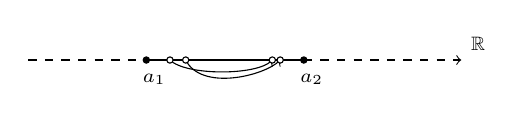
\begin{tikzpicture}
       \path (-1.5,2) coordinate (P);
       \path (4,2) coordinate (Q);
       \path (0,2) coordinate (A);
       \path (2,2) coordinate (B);
       \path (0.3,2) coordinate (M1);
       \path (1.6,2) coordinate (N1);
       \path (0.5,2) coordinate (M2);
       \path (1.7,2) coordinate (N2);
       % real line -------
       \draw [style=dashed] (P) -- (A);
       \draw (A) -- (B);
       % real line -------
       \draw [->][style=dashed](B) -- (Q) node[above right] {\scriptsize{$\R$}}; 
       % boundaries -----
       \draw (A) ++(0.1,-0.05) node[below] {\scriptsize{$a_1$}};
       \draw (B) ++(0.1,-0.05) node[below] {\scriptsize{$a_2$}};
       % circles in A and B -----
       \draw (A) [fill=black] circle (0.04);
       \draw (B) [fill=black] circle (0.04);
       % flow of the middle points ----
       \draw [->](M1)..controls (0.5,1.8) and (1.4,1.8)..(N1);
       \draw [->](M2)..controls (0.7,1.6) and (1.5,1.8)..(N2);
       % middle points -------
       \draw (M1) [fill=white] circle (0.04);
       \draw (M2) [fill=white] circle (0.04);
       \draw (N1) [fill=white] circle (0.04);
       \draw (N2) [fill=white] circle (0.04);
       \end{tikzpicture}
       \end{center}  
 Since the same is true
 for the Cayley transform, namely $\vac^{\R_+}=\vac^{\s_+}\circ C$,
 then the modular flow on the circle is nothing but
 \[
 \sigma_t^{\s_+}=C\circ\sigma_t^{\R_+}\circ C^{-1}.
 \]
 
 \bigskip
 This property ensures that the action of the modular group
 on Fermi fields localised in one interval is geometric. Now
 the question that naturally arises and that we want to address
 is what the modular group is whenever fields are localised
 in different intervals instead. As we shall see, the action
 can no more be geometric because of conflicts with algebraic
 properties otherwise. As first, we introduce the following 
 characterisation of von Neumann algebras due to Takesaki 
 \cite{Tak:1970}
 and we rephrase it in the language of nets with cyclic
 and separating vectors. 
 \begin{definition}[conditional expectation]
 Let $\mathcal{N}\subset\mathcal{M}$ be an inclusion of
 von Neumann algebras and let $\varphi$ be a cyclic and
 separating state on 
 $\mathcal{M}$. A linear map $\mathcal{E}\colon\mathcal{M}
 \to\mathcal{N}$ is called the ``conditional expectation''
 of $\mathcal{M}$ onto $\mathcal{N}$ with respect to
 $\varphi$~if
  \begin{enumerate}
   \item $\varphi\circ\mathcal{E}=\varphi|_{\mathcal{N}}$
   \item $\mathcal{E}(x)=x,\quad x\in\mathcal{N}$
   \item $\mathcal{E}(x) \Omega=P_{\I}\,x\,\Omega
          \quad x\in\mathcal{M}$
  \end{enumerate}
 where $\Omega$ emerges out of the \ac{GNS} representation
 of $\varphi$ and $P_{\I}$ projects onto
 $\hil_{\I}=\set{x\,\Omega\mid x\in\alg{\I}}$.
 \end{definition}
 \begin{theorem}[Takesaki, \cite{Tak:1970}]
 Let $\mathcal{N}\subset\mathcal{M}$ and $\varphi$ as above. 
 The existence of a conditional expectation 
 $\mathcal{E}\colon\mathcal{M} \to\mathcal{N}$ is equivalent
 to the global invariance $\sigma_t^{\varphi}(\mathcal{N})=
 \mathcal{N}$ under the modular automorphism group. 
 \end{theorem}
 Let us now assume we take two (for the sake of simplicity)
 any disjoint intervals $\I_1,\I_2\mid \I_1\cup\I_2\eqqcolon \textrm{E}_2$
 and consider the action of the modular group of the algebra
 $\alg{\textrm{E}_2}$ with respect
 to the vacuum state. The action being still 
 geometric within each of the disjoint intervals
 would imply that $\sigma_t(\alg{\I_k})\subset\alg{\I_k}$ and
 as a consequence conditions for the Takesaki's theorem would
 apply. The Reeh-Schlieder property ensures that the vacuum
 is cyclic and separating for each of the two subalgebras, hence
 the subset $\hil_{\I}$ is dense in $\hil$. Therefore $P_{\I}=
 \bm{1}$ and $\mathcal{E}\Omega=x\Omega,\,x\in\alg{\textrm{E}_2}$.
 Since $\Omega$ is also separating then $\mathcal{E}x=x$ however
 you choose $x\in\alg{\textrm{E}_2}$ and thus $\alg{\textrm{E}_2}$
 must coincide with $\alg{\I_k}$, which is not the case at hand.
 From this we realise that the action of the modular automorphism
 group (with respect to the vacuum state)
 on Fermi fields localised in disjoint intervals cannot be
 \emph{purely} geometric in order to avoid conflicts with
 Takesaki's theorem. We shall see that 
 a mixing with pointwise coefficients is 
 realised with free Fermi fields.
 
 
 
 \subsection{Geometric flow for product states}
 \label{product states}
 Of course, the situation is quite different if we choose
 states that decompose as the product of many vacuum states.
 This choice would destroy all the correlations among different
 intervals and no restrictions given by the Takesaki theorem
 would therefore apply. This issue has been investigated by 
 the authors of \cite{LMR:2009} and we shall summarise 
 here the important results. 
 
 Equipped with a net of Fermi algebras $\I\to\alg{\I}$
 the modular group with respect to the vacuum state
 acts geometrically within each interval on localised fields 
 (Bisognano-Wichmann property), the geometric flow being
 given by the subgroup $\delta_t$ of the M\"obius group preserving
 the interval (dilations on $\I=\R_+$).
 
 \bigskip
 Let $\I$ be an interval on the circle and $\textrm{E}_N=
 \sqrt[N]{\I}$ the symmetric $N$-interval generated,
 i. e. the set of all points $z$ such that $z^N\in\I$. 
 The $N^{\textrm{th}}$ covering of the M\"obius group, as introduced in
 \ref{The Moebius group}, acts on the net as
 \[
 U^{(N)}\left(\Lambda_{\I}^{-2\pi t}\right)\,
 \alg{\textrm{E}_N}\,
 {U^{(N)}\left(\Lambda_{\I}^{-2\pi t}\right)}^*
 =\alg{\delta^{(N)}_t(\textrm{E}_N)}
 \]
 where the geometric flow corresponds to the
 $n$-dilations $\delta_t^{(n)}(z)=\sqrt[n]{\delta_t(z^n)}$.
 Therefore each sub-interval is separately preserved
 by this action. If we assume the net to be split, then
 on $\textrm{E}_N=\I_1\cup\ldots\cup \I_n$ the split
 isomoprhism provides a correspondence 
 $\chi_{\textrm{E}_N}\colon\vee_{k=1}^N\alg{\I_k}\to
 \otimes_{k=1}^N\alg{\I_k}$. With the help of such
 a map we can construct a product state as follows:
 let $U(g_k)$ implement a family of diffeomorphisms acting like
 $z_k\mapsto z^N$ on each of the $\I_k$ and let $\vac$ be the
 respective vacuum state. Define now (\cite{LMR:2009})
 the Kawahigashi-Longo state on the algebra of the
 multi-intervals $\alg{\textrm{E}_N}$ 
 \begin{equation}
 \label{K-L state}
 \varphi_{\textrm{E}_N}\coloneqq 
 \left(\bigotimes_{k=1}^n \vac\circ \ad (U(g_k^{-1}))\right)
 \circ\chi_{\textrm{E}_N}.
 \end{equation}
 The modular automorphisms flow for such a product 
 state is, by construction, geometric within each 
 sub-interval of $\textrm{E}_N$, the geometric flow
 being given by the $N$-dilations:
 \[
 \sigma_t^{\varphi_{\textrm{E}_N}}
 \left(\alg{\I_k}\right)=\alg{\delta_t^{(N)}(\I_k)}.
 \]
 The same construction can be generalised to 
 non-symmetric intervals accordingly. We choose a 
 general family of diffeomorphisms $g_k\colon\I\to\I_k$
 with the property that, given $z\in\I$, then $z_k=g_k(z)\in\I_k$.
 The factorisation is then
 \[
 \varphi_{\textrm{E}_N}\coloneqq 
 \left(\bigotimes_{k=1}^n \vac\circ \ad (U(g_k))\right)
 \circ\chi_{\textrm{E}_N}
 \]
 and the modular group still acts geometrically,
 the geometric flow being now given by
 $\delta_t^{\textrm{E}_N}(z)=(g_k^{-1}\circ 
 \delta_t^{(1)}\circ g_k)(z)$ instead;
 obviously, this reduces to the square root map
 once you go back to $g_k(z)=$ brances of $\sqrt[N]{z}$. 
 However, we are going to examine the issue of non-symmetric
 intervals deeper, later on.
 
 
 \section{The result of Casini and Huerta}
 \label{ResultCH}
 We shall focus henceforth on the modular theory for Fermi fields
 localised in disjoint intervals and the prototype notation
 will be $\psi(x)\in\alg{\textrm{E}_N}$, with 
 $\textrm{E}_N=\I_1\cup\ldots\cup\I_N$. We shall also switch
 very often from the real line picture to the compact picture
 on the unit circle via Cayley transform. Natural notation
 is $\psi(x_k),\,x_k\in\I_k$ (and similarly for $z_k$ on the
 circle) to refer to a field evaluated in $\I_k$.
 
 \bigskip
 As we have seen, whenever
 we consider fields localised in different intervals the action
 of the modular automorphism group with respect to the vacuum state
 cannot be geometric because of conflicts between Takesaki's
 theorem and the Reeh-Schlieder property.
 A priori, for general space-time regions and massive fields, 
 the action of the modular group may be of any fuzzy sort.
 In fact, when conformal invariance no more holds, one cannot 
 transfer the geometric result of Bisognano and Wichmann via 
 conformal mappings and thereby the modular action has to be
 non-local. In particular the authors in \cite{Saf:2006, FigGui:1989} 
 tried to describe the Tomita operators whence the modular 
 automorphisms group comes in terms of pseudo-differential 
 operators, from which the non-local action of the modular 
 group arises. As for the modular group of a multi-interval 
 algebra with respect to the Fock vacuum in free conformal 
 theories, it will still act linearly on the free fields, 
 because the modular operator $S$ preserves the $N$-particle 
 subspaces and hence so does the Tomita operator $\Delta$.
 On the other hand, as we have just seen, it cannot preserve the
 single-interval subalgebras. If we knew that the action is pointwise,
 the most general modular flow would be of the form
 \begin{equation}
 \label{CHmatrix}
  \begin{matrix}
  \sigma_t(\psi(x_1))=&c_{11}(x_1,t)\psi(\zeta_t(x_1))\,+
                     &\ldots&+\,c_{1N}(x_N,t)\psi(\zeta_t(x_N))\\
  \vdots&\vdots&\vdots\\  
  \sigma_t(\psi(x_N))=&c_{N1}(x_1,t)\psi(\zeta_t(x_1))\,+
                      &\ldots&+\,c_{NN}(x_N,t)\psi(\zeta_t(x_N))
  \end{matrix}
 \end{equation}
 or, in a more compact notation,
 \begin{equation}
 \sigma_t \begin{pmatrix}
          \psi(x_1)\\
          \vdots\\
          \psi(x_N)\\
          \end{pmatrix}
 =        \begin{pmatrix}
          c_{11}(x_1,t)&\ldots& c_{1N}(x_N,t)\\
          \vdots&\ddots&\vdots\\
          c_{N1}(x_1,t)&\ldots& c_{NN}(x_N,t)\\
          \end{pmatrix} 
          \begin{pmatrix}
          \psi(\zeta_t(x_1))\\
          \vdots\\
          \psi(\zeta_t(x_1))\\
          \end{pmatrix}.
 \end{equation}
 where $\zeta_t(x)$ is some flow to be determined.
 Of course, once one switches to the circle picture, the 
 entries of the matrix are different. Indeed, the 
 unexpected finding by Casini and Huerta states 
 that for free Fermi fields, the modular flow is of this form.
 
 \bigskip
 The investigation of the modular automorphism group is
 then related to the evaluation of the coefficient appearing
 in \eqref{CHmatrix}. The original paper by \cite{CH:2009}
 provides the calculation of such coefficients using methods
 coming from density matrix and hamiltonian flows. It is 
 known that the time evolution generated by the modular 
 Hamiltonian $K$ of a system, with $\e^{iKt}=\Delta^{it}$  
 satisfies the \ac{KMS} property with 
 respect to the vacuum state and therefore coincides with
 its modular group (for details we refer the reader again to
 \cite{CH:2009} and references therein). Thermal states are 
 characterised by density matrices of the form $\rho\sim 
 \e^{-K}$ and correlators can be expressed as 
 $\scal{\Omega,\blank\Omega}= \tr(\rho\cdot\blank)$. 
 This brings up a relation between the Hamiltonian
 and the $n$-point functions (especially the two-point
 function) that can be used to compute the modular
 dynamics $\comm{K,\psi}$. Exponentiating the commutator
 one gets the entire time evolution $\e^{itK}\psi(x)
 \e^{-itK}$ corresponding to the modular action 
 $\sigma^t_{\vac}(\psi(x))=\Delta^{it}\psi(x)\Delta^{-it}$. 
 As a consequence the argument is that knowledge 
 of the Hamiltonian evolution 
 flow and density matrix allows, at least formally, 
 the computation of the modular automorphisms group in 
 terms of kernel of distributions. 
 
 \bigskip
 Let us consider the algebra of a Fermi field localised 
 in $N$ disjoint 
 open intervals $I_1\cup\ldots\I_N\eqqcolon\textrm{E}_N$,
 with $\I_k=\mathopen{]}a_k,b_k\mathclose{[} \subset \R$;
 we call the interval ``symmetric'' if $\I_k$ are the 
 $N^{\textrm{th}}$
 roots of an interval $\I\subset\R$ (in this case we write
 $\textrm{E}_N=\sqrt[N]{\I}$). 
 Let us introduce the following Casini-Huerta
 function $X\colon\textrm{E}_N\to\R_+$ mapping each of the
 intervals monotonously onto $\R_+$ as
 \begin{equation}
 \label{CHfunction}
 X(x)=-\prod_{k=1}^N\frac{x-a_k}{x-b_k}=
 \prod_{k=1}^N\frac{1+v_k}{1+u_k}\cdot\prod_{k=1}^N
 \frac{z-u_k}{z-v_k}
 \end{equation}
 where $z,u_k,v_k$ are the Cayley images of the points
 $x,a_k,b_k$. Each $X\in\R_+$ has exactly $N$ pre-images,
 one in each interval, and we refer to them as to
 $X_1^{-1}(X),\ldots,X_N^{-1}(X),\ X_j^{-1}(X)\in I_j$. 
 Similarly, we denote by $z_k^{-1}(X)$ the $k^{\textrm{th}}$ 
 pre-image on the circle. Moreover, this function has the
 remarkable property that in case of symmetric intervals,
 namely when $z^N\in\I$ and thus $z_k=\omega_k z\in\I_k$
 with $\omega_k^N=1$, then $X(z^N)=\mu\circ C^{-1}(z^N)$, where
 $\mu$ is a suitable M\"{o}bius function.
 
 \bigskip
 The original result by Casini and Huerta (\cite{CH:2009}
 and \cite{LMR:2009}) states that the modular automorphism
 group with respect to the vacuum state acts on Fermi field as
 \begin{multline}
 \label{MGdisj}
 \sqrt{{X_k^{-1}(X)}'}\,\sigma_t\left(\psi(X_k^{-1})\right)=\\
 \sum_{j=1}^N\,O(X,t)_{kj}\sqrt{{X_k^{-1}(\delta_t(X))}'}
 \psi\left((X_j^{-1}(\delta_t X))\right)
 \end{multline}
 where the flow $\zeta_t(X_k^{-1}(X))$ corresponds
 exactly to the geometric flow appearing in the one interval
 case
 \[ 
 \zeta_t(X_k^{-1}(X))=\delta_t(X_k^{-1}(X))=
 X_k^{-1}(\delta_t(X))
 \]
 with $\delta_t$ being the
 one parameter subgroup of M\"{o}bius transformations
 preserving the interval $\R_+$. The geometric part moving
 the points happens to be the same as in the one interval
 case, plus a mixing among different intervals occurs on 
 top of it. Of course, if one reads the modular flow in 
 terms of hamiltonian evolution, it is easy to understand
 that such an evolution usually delocalises fields in the 
 pure sense of quantum mechanics, and thus we can no more
 expect a geometric action within each subinterval.

 The matrix $O(X,t)$ appearing in \eqref{MGdisj} is an 
 orthogonal cocycle $\in \textrm{SO}(N)$ given in terms of 
 a differential equation (\cite{LMR:2009}) as 
 \begin{equation}
 \label{CHcocycle}
 \partial_tO(X,t)=O(X,t) K(\delta_t X)
 \end{equation}
 where the matrix $K(X)$ on the right hand side is
 \begin{equation}
 \label{matrix_K}
  {K(X)}_{kj}=
  \begin{cases}
  2\pi\,\dfrac{\sqrt{{X_k^{-1}(X)}'\,{X_j^{-1}(X)}'}}
  {{X_k^{-1}(X)} - {X_j^{-1}(X)}}\quad\mbox{if } k\neq j\\
  0\quad\mbox{otherwise}
 \end{cases}.
 \end{equation}
 The solution is a coboundary
 \[
 O(X,t)=O(X)^T\cdot O(\delta_t X)
 \]
 where $O(X)$ is the anti-path-ordered exponential
 \begin{equation}
 \label{anti-path}
 O(X)=\overline{P}\left(\e^{\displaystyle{-\frac{1}{2\pi}
 \int_{X_0}^X\dd X'\,K(X')}}\right).
 \end{equation}
 
 \bigskip
 As a matter of example we can carry out the explicit
 form of this matrix in the case of symmetric intervals.
 In this case, as we have seen, the related points
 $z_k\in\I_k$ are obtained by taking one of the $N^{\textrm{th}}$
 roots of $z^N$, hence $z_k=\omega^k z$, where
 $\omega=\e^{\frac{2\pi i}{N}}$ 
 is the $N^{\textrm{th}}$ root of the unity, $\omega^N=1$
 and $\omega^k=\e^{\frac{2\pi i}{N}k}$. Such points can also
 be obtained out of the Casini-Huerta uniformisation function,
 calculated for symmetric interval, after a suitable
 match with a M\"obius transformation (this is necessary
 whenever the Casini-Huerta function has range $\R_+$, to
 match the M\"obius transformation taking the upper semi-circle
 to the interval $\I$).
 
 However, the symmetric form drastically simplifies 
 the entries of the matrik $K(X)$, as they become 
 \begin{equation}
  {K(z)}_{kj}= 2\pi\,\frac{\omega^{\frac{k+j}{2}}}
  {(\omega^k-\omega^j)z}=-\overline{K}_{kj}\,\frac{1}{z}
 \end{equation}
 with $\overline{K}_{kj}$ a matrix with constant entries
 \[
 \overline{K}_{kj}=-\frac{\omega^{\frac{k+j}{2}}}
  {(\omega^k-\omega^j)};
 \]
 of course ${K(z)}_{kj}$ is still zero if $k=j$.
 Since the matrix $\overline{K}$ is a constant matrix, it
 commutes with itself at different points and as a consequence
 the anti-path-ordered exponential reduces to an ordinary
 exponential
 \begin{equation}
 O(X)=\e^{\displaystyle{\,\frac{1}{2\pi}\,2\pi\,\overline{K}
 \int_1^z \dd w\,\frac{1}{w}}}
 =\e^{\displaystyle{\,\overline{K}\ln z}}=z^{\displaystyle{\overline{K}}};
 \end{equation}
 clearly enough, $z=\e^{i\varphi}$ is any point on the
 circle. The expression we have obtained is rather simple,
 in the case of symmetric intervals; later on we will
 introduce a lemma stating the particular form allowed
 for the spectrum of such a matrix, also calculating
 the particular diagonal form it acquires after an
 orthonormal transformation $K=B^{-1}\,D\,B$, with 
 a unitary matrix $B$ and a diagonal matrix $D$. 
 For the moment we can just plug this expression in the 
 above formula (no matter what these matrices actually are)
 to obtain 
 \[
 z^{\displaystyle{\overline{K}}}=
 z^{\displaystyle{B^{-1}\,D\,B}}=
 \e^{i\varphi\displaystyle{B^{-1}\,D\,B}}=
 B^{-1}\,z^{\displaystyle{D}}\,B
 \]
 and the matrix $D$ can be decomposed over its 
 eigenvalues $\lambda_k$ as $D=\sum_{k=1}^{n}
 \lambda_k\,P_k$, where $P_k\coloneqq \ket{e_k}\bra{e_k}$ 
 is the projection over the $k^{\textrm{th}}$ eigenspace.
 Running once around the circle the change in the variable 
 $z$ is $z\mapsto \e^{2\pi i}z$ and so the matrix $O(z)$
 changes consequently as
 \[
 O(\e^{2\pi i}z)=B^{-1}\,\e^{2\pi i\,
 \displaystyle{\sum_{k=1}^n\lambda_k P_k}}
 \,z^{\displaystyle{\overline{K}}}\,B.
 \]
 We shall see that the spectrum $\lambda_k$ of $D$
 is basically made of natural numbers so that eventually
 one obtains $\e^{(N+1)i\pi}$ and thus we 
 conclude that the only change in the matrix $O(z)$ 
 is up to a minus sign: $O(\e^{2\pi i}z)=(-1)^{N+1}\,O(z)$.
 
 \bigskip
 As we mentioned, the spectrum of the matrix $K(X)$ is 
 given, in the symmetric case, by the following:
 \begin{lemma}[\cite{Rehren:2012wa}]
 The matrix $K(X)$ has integer spaced spectrum 
 $\frac{1-n}{2},\ldots,\frac{n-1}{2}$ in the symmetric
 case. It is diagonalised by the unitary matrix 
 $\frac{1}{\sqrt{n}}B$ whose entries are 
 $B_{kj}=\omega^{(1/2-k)j}$, $\omega$ being given
 by the root of the unity as above. This implies 
 $B\,K=D\,B$, where $D$ is the diagonal matrix
 with entries $D_{kk}=\frac{n+1}{2}-k$.
 \end{lemma}
 \begin{proof}
 By direct computation of the left hand side 
 \begin{multline*}
 \sum_{j\neq l}^n B_{kj}K_{jl}=-
 \sum_{j=l+1}^{n+l-1}\frac{\omega^{(1/2-k)j}
 \omega^{\frac{j+l}{2}}}{\omega^j-\omega^l}\\
 =-\omega^{(1/2-k)l}\sum_{j=1}^{n-1}
 \frac{\omega^{(1/2-k)j}\omega^{\frac{j+2l}{2}}}{(\omega^j-1)\omega^l}
 \end{multline*}
 where we made use of the invariance of the sum under 
 the shift $j\to j+n$. Now we symmetrise again the 
 sum under $j\leftrightarrow n-j$ to have 
 \begin{multline*}
 \sum_{j\neq l}^n B_{kj}K_{jl}=
 -B_{kl}\sum_{j=1}^{n-1}\frac{\omega^{(1-k)j}}{\omega^j-1}\\
 =-B_{kl}\cdot \frac{1}{2}\sum_{j=1}^{n-1}
 \Big(\frac{\omega^{(1-k)j}}{\omega^j-1}+
 \frac{\omega^{(1-k)(n-j)}}{\omega^{n-j}-1}\Big)
 \end{multline*} 
 \noindent Notice now that whenever $z\in\s$ 
 is a phase, contributions of the form 
 \[
 \frac{z^m-z^{-m}}{z-z^{-1}}=z^{m-1}+\ldots 
 +z^{1-m}
 \]
 can be simplified cancelling the denominators. 
 This applies as well to $\omega$ and the 
 right hand side becomes then 
 \[
 -B_{kl}\cdot\frac{1}{2}\sum_{j=1}^{n-1}
 \frac{\omega^{(1-k)j}-\omega^{kj}}{\omega^j-1}
 =B_{kl}\cdot\frac{1}{2}\sum_{j=1}^{n-1}
 \sum_{\nu=1-k}^{k-1}\omega^{j\nu}.
 \]
 Since $\omega^n=1$ we derive that 
 $\sum_{j=0}^n\omega^{j\nu}=n\,\delta_{\nu,0}$
 and thus 
 \[
 \sum_{j\neq l}^n B_{kj}K_{jl}=
 B_{kl}\sum_{\nu=1-k}^{k-1}(n\,\delta_{\nu,0}-1)
 =B_{kl}\cdot\frac{1}{2}(n-2k+1)=D_{kk}\cdot B_{kl}
 \]
 completing the proof.
 \end{proof}


 
 \section{Diffeomorphisms covariance}
 \label{Longo-Xu}
 We shall now turn to a very important feature 
 of conformal nets on the circle which follows 
 from the way fields are assumed to transform 
 under diffeomorphisms. We shall follow the guide 
 lines provided by \cite{LX:2004}: we assume the net
 to be diffeomorphisms covariant and split, i. e.
 for each couple of intervals $\I_1,\I_2$ with 
 disjoint closure, there exist an isomoprhism 
 (the ``split map'') $\chi\colon\alg{I_1}\vee
 \alg{I_2}\to\alg{I_1}\otimes\alg{I_2}$ such that
 $\chi(a_1 a_2)=a_1\otimes a_2$, however you choose
 $a_1\in \alg{\I_1},a_2\in\alg{\I_2}$.
 
 \bigskip 
 Let now $\I$ be an interval on the circle and
 denote as $\mathcal{A}^N(\I)=\alg{\I}\otimes\ldots 
 \otimes\alg{\I}$ many copies of the related algebra.
 We introduce a family of diffeomorphisms 
 $\gamma_j\colon\I\to\I_j$ such that, with natural 
 understanding of notations, given $z\in\I$ then 
 $\gamma_j(z)=z_j\in \I_j$. Diffeomorphisms covariance
 implies the existence of a continuous 
 projective unitary representation of $\Diff(\s)$.
 Once we choose the $\gamma_j$ their action 
 is implemented on the net by means of unitaries 
 $U(\gamma_j)$:
 \[
 \phi^j_I\coloneqq\left.\ad U(\gamma)\right|\alg{\I}=
 \alg{\gamma_j(\I)}=\alg{\I_j}
 \]
 in this respect $\phi^j_I$ is an isomoprhism 
 $\phi^j_I\colon\alg{\I}\to\alg{\I_j}$. Therefore 
 taking the tensor product $N$ times we obtain a map
 \[
 \bigotimes_{k=1}^N \phi_I^k=\phi_I^1\otimes\ldots\otimes
 \phi_I^n\colon\mathcal{A}^N(\I)\to\alg{\I_1}\otimes
 \ldots\otimes\alg{\I_N}
 \]
 acting on the elements as $\phi_I^1(a_1)\otimes\ldots\otimes 
 \phi_I^N(a_N)$. We can now compose everything with 
 the inverse split map $\chi^{-1}$ at our disposal 
 in order to bring $\alg{\I_1}\otimes\ldots\otimes\alg{\I_N}$ 
 into $\alg{\I_1\cup\ldots\cup\I_N}$. The assignment we 
 eventually obtain is called the Longo-Xu map 
 \begin{equation}
 \label{L-X}
 \LX\colon\mathcal{A}^N(\I)\to\mathcal{A}
 (\I_1\cup\ldots \cup\I_N)
 \end{equation}
 and it is explicitly realised on the elements as
 \begin{align*}
 \LX(a_1\otimes\ldots\otimes a_N)&\coloneqq
 \left(\chi^{-1}\circ\bigotimes_{k=1}^N \phi_I^k\right)
 (a_1\otimes\ldots\otimes a_N)\\[1.5ex]
 &=\phi_I^1(a_1)\cdot\ldots\cdot\phi_I^N(a_N) 
 \end{align*}
 for each $a_1,\ldots,a_N\in\alg{\I}$. As a matter
 of example, and very useful for the forthcoming
 purposes, we shall give the explicit formulae
 for the Longo-Xu map in case the diffeomorphisms
 $\gamma_j(z)$ coincide with the inverse root map.
 \begin{example}[Square root map]
 For the sake of simplicity let us restrict to a 
 symmetric two-interval $\sqrt{\I}=\I_1\cup\I_2$, 
 that is the
 set of points $z\in\s$ such that $z^2\in\I$. 
 The diffeomorphism at hand is the square root 
 map $z^2\mapsto \sqrt{z^2}=\pm z$ and we identify
 the two solutions as the two branches $\mu_1(z^2)=
 z$, $\mu_2(z^2)=-z$ and thus the two intervals are
 related to each other as $\I_2=\rot(\pi)(\I_1)$. Also,
 in order to avoid troubles with the discontinuities,
 we require such interval not to contain the point 
 where the cut in the square root is chosen. \\
 
 In particular, if we take two copies $\psi^{(1)},
 \psi^{(2)}$ of a Fermi field localised in $\I$ we have,
 applying \eqref{L-X}
 \begin{align*}
 \LX\left(\psi^{(1)}(z^2)\otimes\bm{1}\right)&=
 \ad U\left(\sqrt{\blank}\right)(\psi^{(1)}(z^2))\cdot\bm{1}\\
 \LX\left(\bm{1}\otimes\psi^{(2)}(z^2)\right)&=
 \bm{1}\cdot\ad U\left(-\sqrt{\blank}\right)(\psi^{(2)}(z^2)).\\ 
 \end{align*}
 By using the conformal transformation law of the 
 Fermi fields, the adjoint action reduces to 
 \[
 \ad U(\gamma)\psi(z)=\sqrt{\frac{\partial\gamma}{\partial z}}
 \,\psi(\gamma(z))
 \] 
 and thus
 \begin{align*}
 \LX\left(\psi^{(1)}(z^2)\otimes\bm{1}\right)&=
 \frac{1}{\sqrt{2z}}\,\psi(z)\\[1.5ex]
 \LX\left(\bm{1}\otimes\psi^{(2)}(z^2)\right)&=
 \frac{i}{\sqrt{2z}}\,\psi(-z).
 \end{align*}
 Even more useful for the next issues is the form this
 map acquires on the complex fermion 
 \begin{align}
 \LX(\phi(z^2))&=\LX\left(\psi^{(1)}(z^2)+i\psi^{(2)}(z^2)\right)
 =\frac{1}{2\sqrt{z}}\left(\psi(z)+\psi(-z)\right)
 \label{LX_complex}\\ 
 \LX(\phi(z^2)^*)&=\LX\left(\psi^{(1)}(z^2)-i\psi^{(2)}(z^2)\right)
 =\frac{1}{2\sqrt{z}}\left(\psi(z)-\psi(-z)\right).
 \end{align}
 \end{example}
 
 \bigskip
 The Longo-Xu map allows us to
 simplify the expression of the Kawahigashi-Longo
 state that we have introduced before, \eqref{K-L state}. 
 In fact, again 
 in case of a symmetric two-interval $\sqrt{I}$, 
 the state \eqref{K-L state} appears to be exactly
 \begin{align*}
 \varphi_{\sqrt{\I}}&=\left(\vac\otimes\vac\right)
 \circ\left(\ad U(z\mapsto z^2)\otimes\ad U(-z\mapsto z^2)\right)
 \circ\chi^{-1}_{\sqrt{\I}}\\ 
 \varphi_{\sqrt{\I}}&=\left(\vac\otimes\vac\right)\circ
 \LX^{-1}
 \end{align*}
 This relation is going to be very useful to compare
 such product state with the vacuum state defined 
 on the algebra of the multi-interval.
 
 \section{A multi-local isomorphism}
 \label{A multi-local isomorphism}
 In this section we present a simple isomorphism between 
 the algebra of one real chiral Fermi field and the algebras 
 of $n$ real chiral Fermi fields in the context of 
 nets of von Neumann algebras. Unlike the Longo-Xu map, 
 this isomorphism preservers
 the vacuum state due to a suitable change of localisation;
 we first prove the result for symmetric intervals and 
 then extend it to the general case of non-symmetric intervals,
 using insights and results from \cite{CH:2009}.
 
 \bigskip
 As a start-up we recall that in general, due to the
 split property, we can make use of the 
 split map between any two algebras $\chi\colon\alg{\I}\vee
 \alg{\textrm{J}}\to\alg{\I}\otimes\alg{\textrm{J}}$
 taking $ab\to a\otimes b$. To be more precise, since we
 shall be dealing with Fermi fields, the tensor product
 $\otimes^t$ is understood to be ``graded'', namely 
 for any two operators $A\otimes^t B$ is the true tensor
 product $A\otimes B$ if either of them is a Bose field, and a 
 twisted tensor product $A\otimes (-1)B$ if both of them 
 are Fermi fields. This is to ensure the correct commutation 
 or anti-commutation relations, respectively. Of course,
 whenever we are dealing with sums of 
 Bose and Fermi fields, the correct formulae for the tensor 
 product follow by linearity.
 
 However, as shown in the previous paraghraph, this is 
 implemented on the algebras as the Longo-Xu map, especially 
 when the fields at hand satisfy diffeomorphisms covariance. 
 Roughly speaking, this allows us to move the fields around the 
 circle and in particular we can bring any number $N$ of 
 ``copies'' of one algebra $\mathcal{A}^N(\I)$ onto 
 one ``delocalised'' copy of the same algebra 
 $\alg{\I_1\cup\ldots\cup\I_N}$ via 
 $\LX(a_1\otimes\ldots\otimes a_N)=
 \phi_I^1(a_1)\cdot\ldots\cdot\phi_I^N(a_N)$.
 It is nevertheless clear though, that such a map does not
 preserve the vacuum state, because product states do
 destroy correlations between fields at different points,
 $\vac(a(x)b(y))\neq \vac(a(x))\cdot\vac(b(y))$. 
 
 The new idea is that, nonetheless, a vacuum preserving 
 isomorphism does exist, it just has to be prepared ad hoc,
 and, interestingly enough, we shall see eventually that it 
 is strongly connected to the Longo-Xu isomorphism 
 through a general gauge transformation. Also, this new 
 isomorphism will be globally defined thanks to its 
 extension to the entire circle. Anyway, before we start we 
 recall once more the standard notations to be used.
 
 \bigskip 
 Let $\mathcal{A}^N(\I)$ denote $N$ copies of an algebra 
 of fields localised in the interval $\I$ on the circle 
 (likewise on the real line, we shall switch the two pictures 
 very often), i. e. $\alg{\I}\otimes\ldots\otimes\alg{\I}$.
 Whenever no representation is explicitly stated we assume 
 the fields to be in their defining vacuum representation, namely 
 $\pi_0(\alg{\I})$. However, we will try to be clear enough 
 throughout. A symmetric interval is essentially an 
 $N^{\textrm{th}}$ root $\sqrt[N]{\I}=\I_1\cup\ldots\cup
 \I_N$ and, with clear understanding of symbols, we 
 refer to $z^N\in\I$ and $z_1,\ldots,z_N$ as the roots 
 in each sub-interval $\I_k$, each of them satisfying 
 $z_k^N=z^N\in\I$. Even clearer is the following 
 notation: the related points $z_k$ can be written 
 as $z_k=\omega^k z$ if $\omega=\e^{\frac{2\pi i}{N}}$
 and $z=\e^{i\varphi}$ is any fixed point $\in \textrm{E}_N$.
 This will ensure that each of those roots 
 ``squares'' to $z^N\in\I$. In the special case of $N=2$
 this reduces to $z^2\in\I$ and $\I_1\cup\I_2$ is the 
 set of points of the form $z,-z$ as the two solutions 
 to $\sqrt{z^2}$.
 
 A non-symmetric interval $\textrm{E}_N$, instead, 
 is simply the union of any $N$ intervals with disjoint closure, 
 wherein the related points $z_k\in\I_k$ need not be 
 roots of $z^N$, rather they are defined as roots 
 of a particular $N$-folded map taking the interval 
 $\I$ onto $\I_1\cup\ldots\cup\I_N$, where each of the 
 $z_k$ appears as one of the solutions of this equation.
 In particular, this assignment will be achieved by means 
 of the Casini-Huerta function \eqref{CHfunction} whose 
 properties have already been stated.  
 
 \bigskip 
 Fields will be considered both on the real line $\R$ and
 on the circle $\s$, the passage from either picture to
 the other being achieved by means of the Cayley
 transform. Conformal fields will consequently change 
 as (the extra factor $i$ is conventional)
 \[
 \phi(z)=\sqrt{-i\frac{dz}{dx}}\,\phi(x)=
 \frac{1-ix}{\sqrt{2}}\,\phi(x).
 \]
 Fields in the compact picture are just a reparametrisation
 of fields on the real line, and the extension to the 
 entire circle depends on the representation. As already 
 introduced in the previous paraghraph 
 \ref{repn of Fermi on the circle}, Fermi fields on the real 
 line posses two faithful representations: the vacuum (Neveu-
 Schwarz) and the Ramond representation, the former extending 
 periodically on the circle, the latter anti-periodically.
 The starting point will be a real chiral Fermi field versus 
 two copies thereof, also seen as a complex fermion again in the 
 sense of \ref{repn of Fermi on the circle}, where all the notations,
 two-point functions and commutation rules have already been 
 stated. Obviously fields must be smeared with suitable 
 functions in order to obtain operators on a Hilbert space;
 nevertheless most of the computations will be clear in the 
 sense of distribution, if not stated otherwise.
 
 Moreover, due to the fact that the fields are assumed to be 
 free (and hence their anti-commutators are multiples of the 
 identity operator) the standard anti-commutation relations 
 can be recovered out of the two-point function as 
 \begin{multline*}
 \omega(\psi(z)\psi(w))+\omega(\psi(w)\psi(z))=
 \omega(\omega(\psi(z)\psi(w))+\\ 
 \omega(\psi(w)\psi(z)))=
 \omega(\ant{\psi(z),\psi(w)})=\ant{\psi(z),\psi(w)}.
 \end{multline*}
 In the case at hand we recover
 \[
 \ant{\psi(z),\psi(w)}=\lim_{\lambda\to 1}
 \left(\frac{1}{z-\lambda w} +\frac{1}{w-\lambda z} \right)=
 \frac{2\pi}{z}\,\delta(\varphi-\theta)
 \]
 if $z=\e^{i\varphi}$ and $w=\e^{i\theta}$, for
 $\varphi,\theta\in\open{-\pi}{\pi}$.
 
%*****************************************
\subsection{The symmetric case}
\label{beta symmetric}
%*****************************************
We start with the symmetric case for $N=2$,
namely $z^2\in\I$ and $z,-z\in\I_1,\I_2$ 
respectively. A complex Fermi field $\phi(z^2),
\phi^*(z^2)$ is localised in $\I$ and a real 
Fermi field $\psi(z)$ in $\sqrt{\I}=\I_1\cup 
\I_2$.
\begin{proposition}[\cite{Rehren:2012wa}]
Let $\phi$ and $\psi$ stand for the complex and real 
fermion in their vacuum representation, as stated 
above. The linear map 
\begin{equation}
\label{beta}
\beta\colon\mathcal{A}^2(\I)
\to\alg{\sqrt{I}}
\end{equation}
given by 
\begin{align}
\phi(z^2)&\mapsto\frac{1}{2}
\left(\psi(z)+\psi(-z)\right)
\label{beta_complex}\\[1ex]
\phi^*(z^2)&\mapsto\frac{1}{2z}
\left(\psi(z)-\psi(-z)\right)
\end{align}
for $z\in\s$, induces an isomorphism of $\textrm{CAR}$
algebras preserving the vacuum state on the different 
algebras: $\vac^{(1)}\circ\beta=\vac^{(2)}$. Note that 
the map is well defined because the right hand sides
are invariant under $z\mapsto -z$.
\end{proposition}
\begin{proof}
We start showing the inverse of such a map: clearly, 
summing up the two sides of the equations we obtain
\begin{align*}
2\,\psi(z)&=2\,\beta(\phi(z^2)) + 2z\,\beta(\phi^*(z^2))\\
2\,\psi(-z)&=2\,\beta(\phi(z^2)) - 2z\,\beta(\phi^*(z^2))\\
\end{align*}
therefore the inverse relation reads
\[
\beta^{-1}\left(\psi(\pm z)\right)=\phi(z^2)\pm z\phi^*(z^2).
\]
The adjoint relation is immediate:
\[
\beta(\phi(z^2))^*=z^2\,\beta(\phi^*(z^2)),
\]
hence $\beta$ preserves the adjoints too.
In terms of the two copies 
$\phi(x)=\left(\psi_1(x)+i\psi_2(x)\right)/\sqrt{2}$
the map $\beta$ can be written as
\begin{align*}
\psi_1(z^2)&\mapsto\frac{1}{2\sqrt{2}}\,\psi(z)
\left(1+\frac{1}{z}\right)+\frac{1}{2\sqrt{2}}\,\psi(-z)
\left(1-\frac{1}{z}\right)\\[1ex]
\psi_2(z^2)&\mapsto\frac{1}{2\sqrt{2}}\,\psi(z)
\left(1-\frac{1}{z}\right)+\frac{1}{2\sqrt{2}}\,\psi(-z)
\left(1+\frac{1}{z}\right)\\
\end{align*}
with inverse given by
\[
\beta^{-1}\left(\psi(\pm z)\right)=\
\psi_1(z^2)(1\pm z) +i\psi_2(z^2)(1\mp z).
\]
Now we turn to the vacuum preserving features. The 
simplest proof proceeds by brute force plugging the 
right hand side of \eqref{beta} into the two-point 
function and evaluating the result:
\begin{align*}
\vac\circ\beta\left(\phi^*(z^2)\phi(w^2)\right)&=
\vac\left(\beta(\phi^*(z^2))\beta(\phi(w^2))\right)\\
&=\vac\left(\frac{1}{2z}(\psi(z)-\psi(-z))\right. \cdot
\left.\frac{1}{2}(\psi(w)+\psi(-w))\right)
\end{align*}
this brings four contributions:
\begin{multline*}
\frac{1}{4z}\left(\vac(\psi(z)\psi(w))-\vac(\psi(-z)\psi(w))\right. \\
+\left. \vac(\psi(z)\psi(-w))-\vac(\psi(-z)\psi(-w))\right)
\end{multline*}
which can be summed up using the formula for the vacuum 
two-point function for the real chiral Fermi field 
\begin{align*}
\vac\circ\beta\left(\phi^*(z^2)\phi(w^2)\right)&=
\frac{1}{4z}\left( \frac{1}{z-w}-\frac{1}{-z-w}\right. 
+\left. \frac{1}{z+w}-\frac{1}{-z+w}\right)\\
&=\frac{1}{4z}\,2\,\left(\frac{1}{z-w}+\frac{1}{z+w}\right)\\
&=\frac{1}{2z}\cdot\frac{2z}{z^2-w^2}=\frac{1}{z^2-w^2}\\
&=\vac\left(\phi^*(z^2)\phi(w^2)\right)
\end{align*}
as to be proven. By exploiting Wick theorem, this 
equality extends to all $n$-points functions, since 
these are just sums of products of two-point functions,
see equation \eqref{wick}. As already pointed out, the 
standard anti-commutation relations follow from this
correlation function, therefore they remain preserved as
well.

\bigskip 
Another proof proceeds by simply looking at Fourier modes. 
In the vacuum representation, where we assume the fields are 
evaluated, we have 
\[
 \phi(z^2)=\sum_{r\in\Z+1/2}\phi_r\,
 {(z^2)}^{-r-1/2},\quad
 \psi(z)=\sum_{r\in\Z+1/2}\psi_r\,
 z^{-r-1/2}.
\]
A simple look at the right hand sides of \eqref{beta} 
displays that, for example,
\begin{align*}
\beta\left(\phi(z^2)\right)&=\sum_{r\in\Z+1/2}\beta(\phi_r)\,
 {(z^2)}^{-r-1/2}=
\frac{1}{2}\left(\psi(z)+\psi(-z)\right)\\[1ex]
&=\frac{1}{2}\sum_{r\in\Z+1/2}\phi_r\,z^{-r-1/2}
\left(1+(-1)^{-r-1/2}\right) \\[1ex]
&=\sum_{p\in\Z}\psi_{2p-1/2}{(z^2)}^{-p}=
\sum_{r\in\Z+1/2}\psi_{2r+1/2}{(z^2)}^{-r-1/2}
\end{align*}
therefore the isomorphism appears as a relabelling 
of the Fourier modes $\phi_r\mapsto\psi_{2r+1/2}$.
Similarly for the adjoint field we have 
$\phi^*_r\mapsto\psi_{2r-1/2}$; the variable $r$
runs into $\Z+1/2$ for the vacuum representation.
In terms of these Fourier modes the anti-commutation
relations read
\[
\ant{\phi_r,\phi^*_s}=\ant{\psi_r,\psi_s}=\delta_{r+s,0}
\]
and a simple look shows that
\[
\ant*{\beta(\phi_r),\beta(\phi^*_s)}=
\ant{\psi_{2r+1/2},\psi_{2s-1/2}}=\delta_{2r+1/2+2s-1/2,0}
=\delta_{r+s,0};
\]
the vacuum state is the only state which is annihilated 
by all $\psi_r, r>0$ and by all $\phi_r,\phi_r^*, r>0$,
respectively. Of course the relabelling does not 
change these conditions and ergo the vacuum is still sent 
into itself. The adjoint relations in terms of modes are
$\phi_r^*=(\phi_{-r})^*$ and we can easily see that, by 
making use of $\beta(\phi(z^2))^*=z^2\,\beta(\phi^*(z^2))$
multiplication by $z^2$ becomes a shift by $-1$ in terms 
of modes, and this is exactly $2r+1/2-1=2r-1/2$, indeed 
what happens to $\phi^*_r$ under the action of $\beta$.

\bigskip 
We have thus shown that $\beta$ is an isomorphism that 
preserves the vacuum state, both in the ``local'' setting
(by looking at the two-point function) and from the 
algebraic perspective of anti-commutators.
This is due to change of localisation from the point 
$z^2$ to the points $z,-z$ with suitable coefficients that
must adjust the form of two-point function eventually. We shall 
see later on that such coefficients will acquire a more
general form described by the Casini-Huerta function 
\eqref{CHfunction} in the context of modular theory and this 
will come as a very special feature; with any other function 
$\I_k\to \I$ the statement is no more true. The 
reduction to special symmetric case brings back the form 
we have just analysed. However, it is 
interesting to show what the map $\beta$ becomes on the 
real line, instead. Since $\R=C^{-1}(\s\setminus\set{-1})$ 
then 
\[
\beta^{\R}=C^{-1}\circ\beta^{\s}\circ C.
\]
The square root assignment $z^2\mapsto\sqrt{z^2}=\pm z$
becomes, after Cayley transform, 
$C^{-1}(z^2)=q(x)=2x/(1-x^2)$, whose two 
``square roots'' are the points $x=C^{-1}(z)$ and
$-1/x=C^{-1}(-z)$.
We have that, on the real line, $\beta^{\R}$ is
\begin{align*}
\phi(q(x))&\mapsto\frac{1}{q(x)}\cdot\frac{1}{1-ix}
\Big(x\psi(x)+i\psi(-1/x)\Big)\\
\phi^*(q(x))&\mapsto\frac{1}{q(x)}\cdot\frac{1}{1+ix}
\Big(x\psi(x)-i\psi(-1/x)\Big)
\end{align*}
and the inverse relation is simply
\[
\beta^{-1}(\psi(x))=\frac{1-ix}{1-x^2}\,\phi(q(x)) +
\frac{1+ix}{1-x^2}\,\phi^*(q(x)).
\]
One might still ask to show why the vacuum correlation 
function is preserved on the real line too; this can be
easily proven by brute force, though we prefer to show a
more elegant solution as follows: the vacuum states on the 
real line and on the circle are related via $\vac^{\R}=
\vac^{\s}\circ C$:
\begin{align*}
\vac^{\R}\circ\beta^{\R}&=\vac^{\s}\circ C\circ\beta^{\R}\\
&=\vac^{\s}\circ C\circ C^{-1}\circ\beta^{\s}\circ C\\
&=\vac^{\s}\circ\beta^{\s}\circ C\\
&=\vac^{\s}\circ C=\vac^{\R}
\end{align*}
as to be proven. \qedhere
\end{proof}
With a little care the result we have just presented can be 
straightforwardly generalised to the case of symmetric $N$-intervals. 
Before we do so, we notice that
a closer look to $\beta$ brings the following inspection to 
the coefficients appearing on the right hand sides:
\begin{align*}
\phi(z^2)&\mapsto \frac{z^0}{2}
\left(\psi(\omega^0 z)+\psi(\omega^1 z)\right)\\
\phi^*(z^2)&\mapsto \frac{z^{-1}}{2}
\left(\psi(\omega^0 z)-\psi(\omega^1 z)\right)
\end{align*}
where we have introduced the roots of the unity $\omega^{0,1}=\pm 1$
as in the fashion previously described. Even more compact
is the form:
\begin{equation*}
\phi^{(k)}(z^2)\mapsto\frac{z^{1-k}}{N}\,\sum_{j=0}^{N-1}
\omega^{(1-k)j}\,\psi(\omega^j z)\qquad k=1,2.
\end{equation*}
Let us now take any symmetric $N$-interval with arbitrary $N$, 
exploiting the form of $\sqrt[N]{z^N}$ with $N$
solutions $z_1,\ldots,z_N$ such that $z_k=\omega^k z\in\I_k$.
Similarly we choose $N$ real Fermi fields lying in $\alg{\I}$ 
which we can pairwise combine into $N/2$ complex Fermi fields:
in formulae we assign $\psi^{(1)}(z^N),\ldots,\psi^{(N)}(z^N)$
such that ${{\phi^{(k)}}^*(z^N)}=\phi^{(N+1-k)}(z^N)$.
Then we just have to propose the same ansatz 
for a symmetric $N$-interval $\beta\colon
\mathcal{A}^N(\I)\to\alg{\sqrt[N]{\I}}$
\begin{equation}
\label{beta_any}
\phi^{(k)}(z^2)\mapsto\frac{z^{1-k}}{N}\,\sum_{j=0}^{N-1}
\omega^{(1-k)j}\,\psi(\omega^j z)\qquad k=1,\ldots,N.
\end{equation}
In terms of the initial fields and in terms of Fourier 
modes this becomes 
\[
\psi^{(k)}(z^N)\mapsto\sum_{r\in\Z+1/2}\psi_{1/2-k + (r+1/2)N}\,
{(z^N)}^{-r-1/2}
\]
which corresponds in turn to a relabelling 
of generators $\psi^{(k)}_r\mapsto\psi_{1/2-k + (r+1/2)N}$.
That this is still a vacuum preserving isomorphism can be
again verified by noting that the renumbering of generators 
does not affect the vacuum, or by direct computation of the 
two-point functions, along the same lines as before.







%*****************************************
%*****************************************
%*****************************************
%*****************************************
%*****************************************

%*****************************************
\subsection{The Ramond sector}
\label{The Ramond sector}
%*****************************************
The real free Fermi field possesses another faithful 
representation of positive energy, the Ramond 
sector, as we have seen in \ref{repn of Fermi on the circle}, 
induced by the \ac{GNS} construction from the 
two-point function \eqref{Ramond}. Fields evaluated
in the Ramond sector will be expressed as 
$\ram{z}$. Obviously, as previously stated, their 
representation on the circle in terms of Fourier modes
has a cut at $z=-1$ and extends anti-periodically on the 
whole $\s$:
\[
\ram{z}=\sum_{n\in\Z}{\psi_{\textrm{R},}}_n \,z^{-n-1/2}.
\]
In principle one could just introduce a new field obtained 
by multiplying the actual Ramond field by $\sqrt{z}$, 
in order to ``cancel'' the cut: $\ram{z}\mapsto 
\sqrt{z}\cdot\ram{z}$ and so 
\[
\ram{z}=\sum_{n\in\Z}{\psi_{\textrm{R},}}_n \,z^{-n}
\]
with two-point function
\[
\omega_{\textrm{R}}(\ram{z}\ram{w})=
\frac{1}{2}\cdot\frac{z+w}{z-w}.
\]
Indeed, if we do so, the transformation law for the new 
defined conformal field under diffeomorphisms 
$z\mapsto \gamma(z)$ changes by an extra factor of $\sqrt{z/\gamma(z)}$.
Commutation relations between modes have the form 
$\ant{{\psi_{\textrm{R},}}_n,{\psi_{\textrm{R},}}_m}
=\delta_{n+m,0}$. In particular, the zero mode squares
to one: $2{\psi^2_{\textrm{R},}}_0=\bm{1}$.

\bigskip 
\begin{proposition}
A similar isomorphism like in \eqref{beta} can be 
introduced as 
\begin{equation}
\label{beta_ramond}
\beta_{\textrm{R}}\colon\pi_0(\alg{\I})\otimes^t 
\pi_{\textrm{R}}(\alg{\I})\to
\pi_{\textrm{R}}\left(\alg{\sqrt{I}}\right)
\end{equation}
taking the tensor product of fields in the vacuum and in 
the Ramond sector and defining
\begin{align}
\ram{z^2}\otimes^t\bm{1}_0&\mapsto\frac{1}{2}
\Big(\ram{z}+\ram{-z}\Big)\\[1ex]
\bm{1}_{\textrm{R}}\otimes^t\pi_0(\psi(z^2))&\mapsto\frac{1}{2z}
\Big(\ram{z}-\ram{-z}\Big).
\end{align}
This isomorphism still preserves the vacuum state in the 
form $\omega_{\textrm{R}}\circ\beta_{\textrm{R}}=
\omega_{\textrm{R}}\otimes\vac$.
\end{proposition}
\begin{proof}
We look again at the Fourier modes and the right hand 
sides present a relabelling ${\psi_{\textrm{R},}}_n\mapsto 
{\psi_{\textrm{R},}}_{2n}$ and ${\psi_{\textrm{R},}}_n\mapsto 
{\psi_{\textrm{R},}}_{2n+1}$, respectively;
this ensures that the correct commutation relations 
and two-point function directly follow.\qedhere
\end{proof}











%*****************************************
%*****************************************
%*****************************************
%*****************************************
%*****************************************
%*****************************************
\subsection{The non-symmetric case}
\label{beta non-symmetric}
%*****************************************
We turn now the attention to the vacuum representation in 
the non-symmetric case 
and try to follow the same arguments as before, in 
order to figure out whether an analogous map, 
playing the role of $\beta$, can be derived for 
non-symmetric intervals.
As we said, we take $\textrm{E}_N$ to be any union
of $N$ disjoint intervals on the real line (likewise
on the circle via Cayley map); thus we are looking for 
\begin{equation}
\label{beta_non-sym}
{\beta}'\colon\mathcal{A}^N(\I)\to\alg{\textrm{E}_N}
\end{equation}
that still preserves the vacuum state
$\vac^{(N)}\circ\beta=\vac\otimes\cdots\otimes\vac$. 

For $N=2$ every non-symmetric two-interval can be 
obtained by applying a M\"obius transformation $\mu$ on a 
symmetric one. Therefore the generic 
$\beta'_2$ is nothing but $\mu\circ\beta_2$ and the vacuum 
preservation is ensured by the fact that any M\"obius 
transformation preserves itself the vacuum state. This 
result in no more true for $N\neq 2$ and in the general 
case we need arguments coming from modular theory to
help our constructions.

\bigskip 
In order to introduce such a map we briefly recall a 
general result: let the intervals be given by 
$\I_k=\mathopen{]}a_k,b_k\mathclose{[} \subset \R$ and define 
the function $X(x),\,x\in \R$ by
\begin{equation}
\label{CHfunction}
X(x) = - \prod_{k=1}^N \frac{x-a_k}{x-b_k}\,.
\end{equation}
This function maps each interval monotonously onto $\R_+$, 
so that every $X\in \R_+$ happens to have exactly $n$ 
pre-images (which we refer to as $X_1^{-1}(X),\ldots,X_n^{-1}(X)$), 
one in each interval, $X_j^{-1}(X) \in I_j$.
We borrow the formulae appearing in \cite{CH:2009} 
for reasons that will become clear later. 
In particular, we look at the 
form of the modular automorphisms group for Fermi fields
localised in disjoint intervals, equation \eqref{MGdisj}
 \begin{multline*}
 \sqrt{{X_k^{-1}(X)}'}\,\sigma_t\left(\psi(X_k^{-1})\right)=\\
 \sum_{j=1}^N\,O(X,t)_{kj}\sqrt{{X_k^{-1}(\delta_t(X))}'}
 \psi\left((X_j^{-1}(\delta_t X))\right).
 \end{multline*}
Here fields are evaluated on the real line as functions 
of the variable $X\in\R_+$. We thus have a collection 
of $N$ fields: $\psi_1(X),\ldots,\psi_N(X)$. The 
map $\beta'$ is explicitly given by
\begin{equation}
\label{map_beta_general}
\beta'(\psi_i(X))= \sum_{r=1}^N {O(X)}_{ir}\,\sqrt{{X_r^{-1}(X)}'}\ 
\psi(X_r^{-1}(X))
\end{equation}
where the mixing matrix $O(X)$ is the solution of 
\eqref{CHcocycle} given in terms of the anti-path
ordered exponential
\begin{equation}
\label{OonK}
O(X)=\overline{P}\,\textrm{exp} \left(-\frac{1}{2\pi}
\int_{X_0}^X \dd X'\ K(X')\right)
\end{equation}
the matrix $K(X)$ being 
\[
{K(X)}_{kj}=
 \begin{cases}
 2\pi\,\dfrac{\sqrt{{X_k^{-1}(X)}'\,{X_j^{-1}(X)}'}}
 {{X_k^{-1}(X)} - {X_j^{-1}(X)}}\quad\mbox{if } k\neq j\\
 0\quad\mbox{otherwise}
 \end{cases}\,.
\]
The idea is that all the information is encoded into the special
form of the function \eqref{CHfunction} and the dependence
of $O(X)$ on $K(X)$ as in \eqref{OonK}. In order to prove that
the above $\beta'$ preserves the vacuum state we  
show the equality of the two-point functions proving that
they satisfy the same differential equation with common initial
conditions. Equality of the two-point function means
\[
(\vac \circ \beta')(\psi_i(X)\,\psi_j(Y))=
\vac^{(2)}(\psi_i(X)\,\psi_j(Y))=\frac{-i}{X-Y}\,\delta_{ij} 
\]
Expanding the left hand side we are led to
\begin{align*}
(\vac \circ \beta')(\psi_i(X)\,\psi_j(Y))=&\,
\vac\left(\sum_{r=1}^N{O(X)}_{ir}\sqrt{{X_r^{-1}(X)}'}
\psi(X_r^{-1}(X))\right.\\ 
& \left.\sum_{s=1}^N{O(Y)}_{js}\sqrt{{Y_s^{-1}(Y)}'}
\psi(Y_s^{-1}(Y))\right)\\   
=&\sum_{r,s=1}^N O(X)_{ir} O(Y)_{js}\sqrt{{X_r^{-1}(X)}'}
\sqrt{{Y_s^{-1}(Y)}'}\\ 
&\vac(\psi(X_r^{-1}(X))\psi(Y_s^{-1}(Y)))\\ 
\overset{!}{=}&\,\vac^{(2)}(\psi_i(X)\,\psi_j(Y))
=\frac{-i}{X-Y}\,\delta_{ij}\,.
\end{align*}
Multiplying both sides by $X-Y$ and taking the 
derivative with respect to $X$ gives 
\begin{multline*}
\sum_{r,s=1}^N O(X)_{ir} O(Y)_{js} \sqrt{{Y_s^{-1}(Y)}'}
\left(\sum_{p\neq r} (X-Y)K(X)_{rp}\sqrt{{X_r^{-1}(X)}'}
\vac(p,s)\right. \\
+ \left.\frac{\partial}{\partial X}\left( (X-Y)\sqrt{{X_r^{-1}(X)}'}
\vac(r,s)\right)\right)=0
\end{multline*}
as a consequence, for each $r,s$ it must be proven that
\footnote{In the following line $\vac(p,s)$ stands for
$\vac(\psi(X_p^{-1}(X))\psi(Y_s^{-1}(Y)))$.}
\begin{multline*}
\sum_{p\neq r} (X-Y)K(X)_{rp}\sqrt{{X_r^{-1}(X)}'}
\vac(p,s)\\
+\frac{\partial}{\partial X}\left( (X-Y)\sqrt{{X_r^{-1}(X)}'}
\vac(r,s)\right)=0.
\end{multline*}
The explicit form of $K(X)$ and the derivatives 
help us to obtain the easier to handle equation
\begin{equation}
\label{finalns}
\frac{1}{2}\frac{(X_r^{-1})''}{(X_r^{-1})'}-\sum_{p\neq r}
\frac{(X_p^{-1})'}{X_r^{-1}-X_p^{-1}}=
\sum_{p=1}^n \frac{(X_p^{-1})'}{X_p^{-1}-Y_s^{-1}}
-\frac{1}{X-Y}
\end{equation}
It is now fundamental that the dependence $X_p^{-1}\equiv
X_p^{-1}(X)$ is given by the function \eqref{CHfunction};
this is because the inverse roots $X_p^{-1}$ appear as roots
of the polynomial ${\mathcal{P}}_X(x)= X\prod_{k=1}^N(x-b_k)+
\prod_{k=1}^N(x-a_k)=0$. After the decomposition in terms of 
its solutions we obtain the useful identity
\[
(X+1)\prod_{k=1}^N (x-X_k^{-1}(X)) = 
{\mathcal{P}}_X(x)= X\prod_{k=1}^N(x-b_k)+
\prod_{k=1}^N(x-a_k)
\]
which in turn becomes, after factorising out 
$\prod_{k=1}^N(x-b_k)$ 
on the RHS and evaluating it in $x=Y$
\begin{equation}
\label{polCH}
\prod_{k=1}^N (Y^{-1}-X_k^{-1}(X))=\prod_{k=1}^N(Y^{-1}-b_k)
\left(\frac{X-Y}{X+1}\right)
\end{equation}
where $Y^{-1}$ is any of the inverse roots of $\mathcal{P}(Y)$.
This equation is the starting point to obtain both sides of
\eqref{finalns} as follows: taking the derivative with respect to
$X$ of the logarithm of \eqref{polCH} gives back
\[
\sum_{k=1}^N\frac{(X_k^{-1})'}{X_k^{-1}-Y^{-1}}=
\frac{1}{X-Y} - \frac{1}{X+1}
\]
therefore the right hand side of \eqref{finalns} turns out 
to be nothing but $-1/(X+1)$. Obtaining the right hand side
is slightly trickier and we proceed as follows: we start 
again from \eqref{polCH} taking the logarithm and derivative
with respect to $X$ and then we multiply both sides 
by $(X-Y)(X_j^{-1}-Y^{-1})$. This gives 
\begin{multline*}
(X-Y)(X_r^{-1})' +\sum_{p\neq r} \frac{(X_p^{-1})' 
(X_r^{-1}-Y^{-1})(X-Y)}{X_p^{-1}-Y^{-1}}=\\
X_r^{-1}-Y^{-1} - \frac{(X_r^{-1}-Y^{-1})(X-Y)}{X+1}
\end{multline*}
from which we take again the derivative with respect to
the variable $X$ twice and eventually evaluate it in the
point $Y^{-1}=X_r^{-1}$ (and therefore $Y=X$). In the summation
term we make use of $(ND^{-1})'' = N'' D^{-1}$ whenever both
$N$ and $N'$ vanish in the limit (which is the case at hand).
Carrying the algebra out gives
\[
2 (X_r^{-1})'' - 2 \sum_{p\neq j} \frac{(X_p^{-1})'(X_r^{-1})'}
{X_r^{-1}-X_p^{-1}}= (X_r^{-1})'' - \frac{(X_r^{-1})'}{X+1}
\]
namely nothing but \eqref{finalns}. Now we are left with the 
common initial conditions to be proven (we choose $X=Y$): 
once again, equality of the two-point function 
$\vac\circ\beta'=\vac^{(2)}$ reads
\[
\sum_{r,s=1}^N O(X)_{ir} O(Y)_{js}\sqrt{{X_r^{-1}(X)}'}
\sqrt{{Y_s^{-1}(Y)}'}\,\frac{-i}{X_r^{-1}-Y_s^{-1}}
=\frac{-i}{X-Y}\,\delta_{ij}.
\]
Multiplying both sides by $X-Y$ and splitting the sum into
$r=s$ and $r\neq s$ leads us to
\begin{multline*}
\lim_{X\to Y}\ \sum_{r=1}^N\left(\sum_{r\neq s} 
O(X)_{ir} O(Y)_{js}\sqrt{{X_r^{-1}(X)}'} \sqrt{{Y_s^{-1}(Y)}'}
\frac{X-Y}{X_r^{-1}-Y_s^{-1}}+\right.\\
\left. O(X)_{ir} O(Y)_{jr}\sqrt{{X_r^{-1}(X)}'} \sqrt{{Y_r^{-1}(Y)}'}
\frac{X-Y}{X_r^{-1}-Y_r^{-1}}\right)=\delta_{ij}.
\end{multline*}
The first term vanishes in the limit, whereas the 
divergence in the second term gives back $1/(Y_r^{-1})'$ 
which cancels the square roots. Orthogonality of the 
matrix $O(Y)$ ensures then the result.

\bigskip 
The symmetric case on the circle can be recovered as 
a special case of the general one. In fact the evaluation 
of $X(z)$ turns out to be the composition of the inverse 
Cayley transform with a M\"obius transformation onto $\R_+$.
Using trigonometric identities like $\prod^N_{k=1}(z-\omega_k)
=z^N-\omega^N$ we find 
\[
X(z)=-\frac{(-1)^N-v^N}{(-1)^N-u^N}\cdot 
\frac{z^N-u^N}{z^N-v^N}
\]
which is indeed a M\"obius transform of 
$\frac{z^N-1}{i(z^N+1)}=C^{-1}(z^N)$. Therefore 
\[
X(x)=(C^{-1}\circ\mu\circ(z\mapsto z^N)\circ C)(x)
\]
where $\mu\colon\I\to\textrm{S}^1_+$ is the M\"obius 
transform of the said form. In the general non-symmetric
case the map $z\mapsto z^N$ is replaced by any general
$N$-folded map $g$
\[
X(x)=(C^{-1}\circ\mu \circ g\circ C)(x)
\]
and $\mu$ here is arbitrary. The passage from the circle 
to the real line, in the explicit formulae of $\beta'$, is 
then achieved with the help of suitable M\"obius transformations,
which do not affect the vacuum state. Consequently the 
invariance of the vacuum two-point function on the real line
ensures the same statement on the circle, and viceversa.

\bigskip 
The existence of an isomorphism $\mathcal{A}^N(\I)\to
\alg{\textrm{E}_N}$ preserving the vacuum state implies that
the corresponding \ac{GNS} vacuum representations are 
isomorphic as well. This, in turn, produces a homomorphism 
of many copies of the local algebra of a single 
theory into the algebra of a single fermion localised
in many intervals, represented on the Fock space.


















%*****************************************
%*****************************************
%*****************************************
%*****************************************
%*****************************************
%*****************************************
\subsection{Multi-local fermionisation and 
gauge transformations}
\label{multi-local fermionisation}
%*****************************************
The multi-local isomorphism $\beta$ provides 
a correspondence between fermions localised 
essentially at our will. As we have seen, Fermi 
theories sort of automatically contain (non)-abelian
current algebras, due to the fact that these can 
be embedded using the standard quarks construction
from sufficiently many free fermions.

This feature, in its general behaviour, is referred to 
in the literature as ``fermionisation'', since it 
allows to express bosons (the currents) in terms 
of products of Fermi fields. In particular currents 
are expressed as Wick products (equation \eqref{current})
with subtraction of the vacuum expectation value;
since $\beta$ preserves the vacuum state it extends to
Wick products and therefore embeds 
the currents giving rise to a new feature which is
the delocalisation of the components of the current
itself. We shall be more precise showing the 
construction of such objects on the circle, because
most of the formulae drastically simplify.

\bigskip
Let us start from the vacuum representation and
take the case $N=2$; we look in particular at 
symmetric intervals, for the sake of simplicity, 
though the same construction can be easily generalised
with different coefficients eventually. In terms of the 
complex fermion the current is expressed as
\begin{equation}
\label{curr_complex}
j(z)\coloneqq \wick{\phi^*\phi}(z)=
i\,\wick{\psi_1\psi_2}(z);
\end{equation}
we are going to embed such formula with the help 
of \eqref{beta}. As so, we have (we evaluate on $z^2$
due to $\beta$) 
\begin{align*}
\beta(j(z^2))&=\beta\left(\wick{\phi^*\phi}(z^2)\right)\\
&=\beta\left(\phi^*(z^2)\phi(z^2)-\vac(\phi^*(z^2)\phi(z^2))\right)\\
&=\beta(\phi^*(z^2))\beta(\phi(z^2))-
  \vac\circ\beta(\phi^*(z^2)\phi(z^2))\\
&=\wick{\beta(\phi^*)\beta(\phi)}(z^2).
\end{align*}
The feature of $\beta$ to preserve the vacuum state means that 
it can be taken into the Wick product
due to commutativity $\beta\circ\wick{\blank}=\wick{\blank}
\circ\beta$. Consequently we have
\begin{align*}
\beta(j(z^2))&=\wick{\frac{1}{2z}
\left(\psi(z)-\psi(-z)\right)\frac{1}{2}
\left(\psi(z)+\psi(-z)\right)}\\
&=\frac{1}{4z}\,\wick{\psi(z)^2-
\psi(-z)\psi(z)+\psi(z)\psi(-z)-\psi(-z)^2}
\end{align*}
Fermions anti-commute and so $\psi(z)^2=\psi(-z)^2=0$;
moreover we have $-\psi(-z)\psi(z)=\psi(z)\psi(-z)$.
Making use of such relations we come to the 
\emph{multi-local fermionisation} formula on the 
circle:
\begin{equation}
\label{multi-local_fermionisation}
\beta(j(z^2))=\frac{1}{2z}\,\wick{\psi(z)\psi(-z)}
\end{equation}
The same expression, evaluated on the real line, looks like:
\[
\beta(j(q(x))= \frac{-i}{2x}\cdot\frac{(1-x^2)^2}{(1+x^2)}
\,\wick{\psi(x)\psi(-1/x)}\,.
\]
The current embedded with the isomorphism $\beta$
happens to be delocalised in two anti-podal points
on the circle, $z$ and $-z$. This feature justifies 
the term ``multi-local'' fermionisation (also in
\cite{Rehren:2012wa}) here and henceforth, because
the fermionisation is shared between pairs of 
different points. We notice that this new representation 
of the current is periodic on the circle 
under the change $z\to -z$;
in fact, both numerator (due to the anti-commutators)
and denominator acquire a minus sign, cancelling each
other altogether. Furthermore, since the expectation value 
of a Wick product is always zero, we still have 
$\vac\circ\beta (j(z^2))=0$. On the other hand the 
two-point function is 

\begin{align*}
\vac\circ\beta(j(z^2)j(w^2))&=
\frac{1}{4zw}\,\vac(\wick{\psi(z)\psi(-z)}\,
\wick{\psi(w)\psi(-w)})\\[1ex]
&=\frac{1}{4zw}\,\big(\vac(
\bcontraction{}{\psi(z)}{\psi(-z)\psi(w)}{\psi(-w)}
\bcontraction[2ex]{\psi(z)}{\psi(-z)}{}{\psi(w)}
\psi(z)\psi(-z)\,\psi(w)\psi(-w))\\
&\quad-\vac(
\bcontraction{}{\psi(z)}{\psi(-z)}{\psi(w)}
\bcontraction[2ex]{\psi(z)}{\psi(-z)}{\psi(w)}{\psi(-w)}
\psi(z)\psi(-z)\,\psi(w)\psi(-w))\Big)\\[1ex]
&=\frac{1}{4zw}\,\Big(-\vac(\psi(z)\psi(w))\cdot 
\vac(\psi(-z)\psi(-w))\\
&\quad+\vac(\psi(z)\psi(-w))\cdot
\vac(\psi(-z)\psi(w))\Big)\\[1ex]
&=\frac{1}{4zw}\cdot\frac{4zw}{(z^2-w^2)^2}
=\vac(j(z^2)j(w^2))
\end{align*}
that is, the two-point function is preserved too.

\bigskip 
The embedded current can be decomposed into Fourier modes
on the circle
\[
\beta(j(z^2))=\frac{1}{2z}\sum_{m,k\in\Z+1/2}^N
\wick{\psi_m\psi_k}(-1)^{-k-1/2}z^{-m-k-1}
\]
if $m+k=n$ is odd then $(-1)^{k-n-1/2}=
(-1)^{-k-1/2}$ and the sum vanishes because of 
the anti-commutation relations: each contribution
has its own opposite. Therefore the only allowed
powers of $m+k$ are even powers of the form $m+k=2p$, 
which lead us to 
\[
\beta(j_n)=\sum^{\infty}_{m=0}\psi_{n-m-1/2}\,
\psi_{n+m+1/2}(-1)^{n+m+1}.
\]
The complex fermion is invariant under gauge 
transformations generated by its own embedded 
currents: if $j(z)=\wick{\phi^*\phi}(z)$ then
Weyl-type operators are implemented by
smearing with suitable test functions $f\colon\s\to\R$
in order to obtain $W(f)=\e^{ij(f)}$. Gauge
transformations are then given by
\begin{align*}
\phi'(z)&=\alpha_f(\phi(z))=W(f)\phi(z)W(f)^*
=\e^{-if(z)}\phi(z)\\
{\phi^*}'(z)&=\alpha_f(\phi(z)^*)=W(f)\phi(z)^*W(f)^*
=\e^{if(z)}\phi(z).
\end{align*}
It is now very interesting to embed the gauge 
transformations themselves with the help of $\beta$,
in order to bring new delocalised gauge symmetries,
a brand new feature that we are going to present and 
fully exploit. If $\beta$ embedds the current then it
generates embedded gauge transformations on the free
fermion of the form
\begin{align*}
\beta(W(f))\psi(z)\beta(W(f))^*&=(\beta\circ\alpha_f\circ 
\beta^{-1})\psi(z)\\
&=(\beta\circ\alpha_f)(\phi(z^2)+z\,\phi(z^2)^*)\\
&=\beta(\alpha_f(\phi(z^2)) + z\,\alpha_f(\phi(z^2)^*))\\
&=\e^{-if(z^2)}\beta(\phi(z^2))+z\,\e^{if(z^2)}
\beta(\phi(z^2)^*)
\end{align*}
eventually we end up with
\begin{equation}
\label{emb_gauge}
\beta(W(f))\psi(z)\beta(W(f))^*=
\cos{f(z^2)}\psi(z)-i\sin{f(z^2)}\psi(-z).
\end{equation}
The new remarkable feature is the bilocal mixing
of $\psi(z)$ and $\psi(-z)$, reflecting the 
non-locality of the isomorphism $\beta$.
Of course the same calculations can be performed 
in the situation $N>2$: in this case non-abelian 
currents of the form $j_{rs}(z)\coloneqq
\wick{\phi_r^*\phi_s}(z)$ can be embedded and we
obtain representations of all these theories in 
the Fock space of a single real free fermion. In the 
many interval case $\beta$ delocalises the fields
onto $2N$ points (equations \eqref{beta_any} and,
in general, \eqref{map_beta_general}) and therefore 
expressions like $\wick{\phi_r^*\phi_s}(z)$ present 
sums of fields in pairwise coupled points
$\psi(z_j)\psi(z_l)$ with position dependent 
coefficients. Gauge transformations change 
accordingly, having multi-local contributions 
from different points. 

\bigskip 
The same argument can be run in the Ramond sector:
the fact that the current $j(z)\coloneqq 
\wick{\phi^*\phi}(z)=i\,\wick{\psi_1\psi_2}(z)$
satisfies commutation relations in purely algebraic
and independent of the representation. As a consequence 
one can then take the two fields $\psi_1$ and $\psi_2$ in two
different representations and \emph{twist} the 
product. In fact, by taking $\psi_1$ in the vacuum
sector and $\psi_2$ in the Ramond one, the 
isomorphism \eqref{beta_ramond} embeds the 
resulting current into the Ramond algebra 
$\pi_{\textrm{R}}\Big(\alg{\sqrt{\I}}\Big)$. The Wick 
product here is defined as the subtraction with 
respect to the corresponding Ramond two-point function; 
the result is, in the compact picture:
\[
\beta_{\textrm{R}}(j(z^2))=\frac{1}{2i z^2} \cdot 
\wick{\ram{z}\ram{-z}}_{\textrm{R}}.
\]
The new current, as expected, is delocalised at two 
anti-podal points in the Ramond representation; the 
Wick product is essentially the standard operator 
product, because the Ramond expectation value vanishes
at the case at hand in the points $z,-z$. Also, the 
formula changes sign under $z\to -z$, i. e. it is
anti-periodic in the variable $z^2$, expressing the fact
that the new current is twisted. Of course, the one-point 
function is still zero, whereas the two-point function 
becomes now:
\begin{align*}
\omega_{\textrm{R}}\circ\beta_{\textrm{R}}
(j(z^2)j(w^2))&= -\frac{1}{4z^2w^2}\,\omega_{\textrm{R}}
(\wick{\ram{z}\ram{-z}}\\
&\wick{\ram{w}\ram{-w}})\\[1ex]
&=\frac{1}{2zw}\cdot\frac{z^2+w^2}{(z^2-w^2)^2}
\end{align*}
after making use of the usual Wick contractions within the 
expectation value. This formula has been previously
mentioned by \cite{Ang:2011} as the ``twisted'' 
representation of the current, in the context of
vertex operator algebras (we refer the reader to 
the references therein).










%*****************************************
%*****************************************
%*****************************************
%*****************************************
%*****************************************
%*****************************************
\subsection{Multi-local diffeomorphisms}
\label{Multi-local diffeomorphisms}
%*****************************************
In the previous paraghraph we showed the construction
of the multi-local current and the resulting 
multi-local fermionisation and gauge transformations.
It is natural to extend the investigation 
to the stress-energy tensor of such a theory and 
look for the corresponding multi-local diffeomorphisms
that are generated. Again, the special case $N=2$ for
symmetric intervals is a guideline, because formulae
simplify and this allows to better understand the 
features and the behaviours without getting lost in 
the nasty coefficient for the general case. Fundamental
is again the characteristic of $\beta$ to preserve the
vacuum state in order to be extended to Wick products:
$\beta\circ\wick{\blank}=\wick{\blank}
\circ\beta$.

\bigskip
We start in the vacuum representation, as usual. 
The real free fermion contains the stress-energy tensor
of central charge $c=1/2$ 
\[
T^{1/2}(z)\coloneqq \frac{-1}{4\pi}\,
\wick{\psi\partial_z \psi}(z)
\]
whereas the complex fermion is, roughly speaking, two
copies thereof, with $c=1$
\[
T^{c=1}(z)\coloneqq \frac{-1}{4\pi}\,
\wick{\psi_1\partial_z \psi_1}(z)+
\frac{-1}{4\pi}\,
\wick{\psi_2\partial_z \psi_2}(z)=
\frac{-1}{4\pi}\,\wick{\phi^*
{\overset{\leftrightarrow}{\partial_z}}\phi}(z).
\]
In terms of the currents, the stress-energy tensor 
can be expressed as
\[
T(z)=\frac{1}{4\pi}\wick{j^2}(z),
\]
that is nothing but the abelian version of \eqref{SET}.

The action of $\beta$ brings to the 
embedded stress-energy tensor which we compute to be
\begin{align*}
\beta\big(T^{1}(z^2)\big)&=\frac{-1}{4\pi}\,
\beta\big(\wick{\phi^*
{\overset{\leftrightarrow}{\partial_z}}\phi}(z)\big)\\[2ex]
&=\frac{-1}{4\pi}\,\wick{\beta(\phi(z^2)^*)
\partial_{z^2}\beta(\phi(z^2))
-\partial_{z^2}(\beta(\phi(z^2)^*))\beta(\phi(z^2))}\\[2ex]
&=\under{\sim\beta(j(z^2))}
{\frac{-1}{4\pi}\,\frac{1}{2z^3}
\wick{(\psi(z)-\psi(-z))(\psi(z)-\psi(-z))}}\\
&+\frac{-1}{4\pi}\cdot\frac{1}{4}\cdot\frac{1}{2z^2}
\wick{\Big((\psi(z)-\psi(-z))\partial_z(\psi(z)+\psi(-z))-\\
&(\partial_z(\psi(z)-\psi(-z)))(\psi(z)+\psi(-z))\Big)}\\[2ex]
&=-\frac{1}{8\pi z^2}\beta(j(z^2))+
\frac{1}{4z^2}\big(T^{1/2}(z)+T^{1/2}(-z)\big),
\end{align*}
expressed as embedding of two real fermions of central 
charge $c=1/2$. The remarkable feature is the presence 
of two delocalised
stress-energy tensors in $z,-z$ plus an additional 
contribution proportional to the embedded 
current. We shall see later that this further term can
be cancelled out by composition with a particular 
automorphism of the current algebra, though.

\bigskip
The real and complex fermions are invariant under 
diffeomorphisms generated by its own stress-energy 
tensor. If $f\colon\s\to\s$ is a general diffeomorphism,
then the unitary operators $V(\gamma_t)=\e^{itT(f)}$ implement
its action as
\begin{equation*}
 \psi'(\gamma(z))=\delta_{\gamma}(\psi(z))=
 V(\gamma)\psi(z)V(\gamma)^*
 =\sqrt{\gamma'(z)}\,\psi(\gamma(z))
\end{equation*}
where $i f(z)/z\in\R$ integrates to
diffeomorphisms given by the one-parameter group 
$\partial_t\gamma_t(z)=-(f\circ\gamma_t)(z)$. 
Also, $\gamma(z)$ is meant as $\gamma_t|_{t=1}(z)$.
Simpler to write down is its 
infinitesimal action $\delta_f^0$ expressed by the 
commutator
\[
\delta_f^0(\psi(z))=i\,\comm*{T(f),\psi(z)}=
\Big(-f(z)\partial_z -\frac{1}{2}f'(z)\Big)\psi(z).
\]
We can now make use of the equation for the 
embedded stress-energy tensor 
\begin{equation}
\label{embedded_SET}
\beta\big(T^1(z^2)\big)=-\frac{1}{8\pi z^2}\beta(j(z^2))+
\frac{1}{4z^2}\big(T^{1/2}(z)+T^{1/2}(-z)\big)
\end{equation}
in order to derive and calculate the 
corresponding multi-local diffeomorphisms.
Similarly to the case of currents we have
the action
$i\,\comm*{\beta\big(T^1(f)\big),\psi(z)}=
(\beta\circ\delta_f^0\circ\beta^{-1})\,\psi(z)$.
The contribution due to the two anti-podal parts
$T^{1/2}(z)$ and $T^{1/2}(-z)$ gives rise to
a term proportional to $\delta_f^0(\psi(z^2))$, 
while the contribution proportional to the 
embedded current gives back two anti-podal terms
in $\psi(z), \psi(-z)$; in details we obtain 
\begin{align*}
i\,\comm*{\beta\big(T^1(f)\big),\psi(z)}&=
(\beta\circ\delta_f^0\circ\beta^{-1})\,\psi(z)\\[2ex]
&=\Big(-\frac{1}{2z}\,f(z^2)\partial_z -\frac{1}{2}
f'(z^2)\Big)\psi(z)\\
&+\frac{1}{4z^2}\,f(z^2)\, 
\big(\psi(z)-\psi(-z)\big).
\end{align*}
Again, we have a mixing of $\psi(z)$ and $\psi(-z)$ 
(due to the current), on top of a geometric action 
due to the stress-energy tensor itself. Of course, in
equation \eqref{embedded_SET} everything is 
expressed in terms of the two real copies 
$\psi_1,\psi_2$ of the free fermion; nevertheless 
one can work it back in terms of the complex
fermion $\phi(z),\phi(z)^*$: in this case, 
when acting with the inverse action $\beta^{-1}$, terms 
proportional to $\wick{\phi^*\partial_z\phi}(z)$
will appear and therefore we will have eventually
mixed pairings $\phi,\phi^*$ expressing some sort
of multi-local ``charged'' conjugation.

As previously mentioned (see chapter  
\ref{The quarks construction}), 
the current algebra possesses
automorphisms of the form 
\[
\rho^q(j(z))=j(z)+\frac{q}{z},\qquad q\in\R
\]
which give rise to charged states $\omega_q
\coloneqq\vac\circ\rho^q$. On the actual Weyl 
operators those automorphisms are realised as
\[
\gamma_q(W(f))=\e^{i\rho^q(j(z))(f)}=
\e^{iq\int_{\s}\dd z \frac{f(z)}{2\pi i z}}\,W(f),
\]
giving rise to different inequivalent representations
whenever one chooses $\gamma_{q_1},\gamma_{q_2}$ with 
$q_1\neq q_2$. Moreover, these automorphisms happen to be
even innerly implemented by unitaries if a real function 
$\varphi$ exists such that $q/z=-i\varphi'(z)$
\[
\gamma_{q}\blank=\ad(W(-\phi))\blank
\]
and $\gamma_q(\alg{\I})=\alg{\I}$. In fact the above equation
can be taken as definition for each representation
$\gamma_q(W(f))$ (\cite{Ca2004}). However, since the  
stress-energy tensor is contained as embedded into
the theory of currents, it turns out that 
composition of $\beta$ with such a $\rho^q$
exactly ``undoes''  the additional contribution
due to the current in \eqref{embedded_SET} if
we shift back $j(z)\mapsto j(z)+q/z$ for 
$q=1/4$. The price to pay is the appearance
of a constant shift $\sim z^{-4}$:
\[
\beta\circ\rho^{1/4}\big(T^1(z^2)\big)=
\frac{1}{4z^2}\big(T^{1/2}(z)+T^{1/2}(-z)\big)+
\frac{1}{64\pi z^4}.
\]
Although we have not introduced the issue yet, we want
to emphasise that the constant term popping up 
is nothing but the Schwarz derivative of the square root 
automatically generated because the stress-energy tensor is a 
quasi-primary field. In fact the above formula will
coincide with the Longo-Xu map applied to a doubled 
theory of stress-energy tensors, as we shall see later on
in paraghraph \ref{Embedding via Longo-Xu map}.

Anyway, it is always very useful to rephrase the 
picture in terms of Fourier modes: as known, 
$T^1(z)=1/2\pi\,\sum_{n\in\Z}L^1_n z^{-n-2}$; then 
the embedding looks like, in terms of Virasoro
generators:
\[
\beta(L_n^1)=-\frac{1}{4}\beta(j_n)+
\frac{1}{2}L_{2n}^{1/2}
\]
for the general case, and 
\begin{multline*}
\beta\circ\rho^{1/4}(L_n^1)=-\frac{1}{4}\beta(j_n)+
\frac{1}{2}L_{2n}^{1/2} +\\ \Big(\frac{1}{4}\beta(j_n)+
\frac{1}{32}\delta_{n,0}\Big)=
\frac{1}{2}L_{2n}^{1/2}+
\frac{1}{32}\delta_{n,0}
\end{multline*}
for the subtracted $q=1/4$ current. Here 
the subtraction of the current modes due to the composition
with a charged automorphism is even more evident. 
In contrast, the first (general)
formula involves also the modes of the current, still, which 
may in turn be expressed in terms of the real Fermi fields.
This emphasises that the embedded diffeomorphisms come
along with embedded gauge transformations, i. e. a mixing
of $\psi(z)$ and $\psi(-z)$, as described before.

\bigskip 
In the Ramond sector the stress-energy tensor presents
an additional term by definition, as shown in equation 
\eqref{SET_vac_vs_R}. Consequently, the action of 
$\beta_{\textrm{R}}$ produces different subtractions 
that cancel the gauge term $\beta(j(z^2))$ which we 
had to deal with in the vacuum sector. 
As such, the formula in the Ramond representation 
becomes easier even without composition with a charged
automorphism of the currents:
\[
\beta_{\textrm{R}}\big(T^1(z^2)\big)=
\frac{1}{4z^2}\Big(\pi_{\textrm{R}}\big(T^{1/2}(z)\big)
+\pi_{\textrm{R}}\big(T^{1/2}(-z)\big)\Big)+
\frac{1}{64 \pi z^4}.
\]

\bigskip 
Finally, a last remark to conclude this section:
the expression of the multi-local 
transformations in terms of Virasoro generator is 
very useful to understand a brand new picture, which
will be pretty convenient when we shall turn to modular
theory. The subgroup $L_0,L_{\pm 1}$ of the Virasoro 
algebra generates the M\"obius group, which in turn
contains rotations, dilations and translations. Its 
multi-local version, given by $\beta(L_0),\beta(L_{\pm 1})$
produces the corresponding multi-local rotations,
dilations and translations. The passage between a single
theory in one interval to a delocalised theory in many
intervals can then by achieved making use of
the same formulae, just taking care of replacing
$L_n\mapsto \beta(L_n)$. The multi-local behaviour
will then be taken into account by the presence of 
$\beta$, automatically, producing mixing among different
components all the time.















%*****************************************
%*****************************************
%*****************************************
%*****************************************
%*****************************************


\section{Multi-local modular theory for Fermi fields}
The most remarkable feature of $\beta$ is that it 
preservers the vacuum state, and therefore its action 
extends to Wick products and so forth, giving rise to 
multi-local transformations among different intervals. 
So far we have not introduced any correspondence with 
modular theory yet, but as we are going to see, very 
important applications can be derived implementing the 
Bisognano-Wichmann property under the action of $\beta$. 
In fact, the modular theory for one-dimensional fermions
is well known and has been widely investigated,
producing the famous result that the action of the 
modular group with respect to the vacuum state 
on the algebra localised in one interval is geometric
within the interval and can be expressed in terms of 
dilations preserving the interval. The interesting idea is that, 
since $\beta$ \emph{moves}
the theory from one interval to many, preserving the 
vacuum state, we can expect a rationale to describe 
the modular theory for Fermi fields localised in many 
disjoint intervals on the circle (respectively on 
the real line). In order to characterise the topic 
in detail we are going to introduce a very strong result,
which is going to play a pretty fundamental role: whenever
two states of two algebras $\mathcal{A}_1,\mathcal{A}_2$ 
are intertwined by an isomorphism, such 
isomorphism also intertwines the modular groups of the two algebras.
\begin{theorem}
If $\beta\colon\mathcal{A}^N(\I)\to\alg{\textrm{E}_N}$
is a vacuum preserving isomorphism, then it intertwines
the respective modular groups:
$\sigma_N^t=\beta\circ\sigma_1^t\circ\beta^{-1}$.
\end{theorem}
\begin{proof}
The proof proceeds by verifying the \ac{KMS} property
for $\sigma_N^t$ with respect to the composed state
$\vac\circ\beta$. Therefore, let 
\[
F^N_{a,b}(t)\coloneqq F^{\vac\circ\beta}_{a,b}(t)=
\scal*{\Omega,\beta^{-1}(a)\beta^{-1}(\sigma_N^t(b))\Omega}
\]
be the \ac{KMS} functional we have to look at, for
$a,b\,\in\alg{\textrm{E}_N}$.
We have to prove that $F^N_{a,b}(t)$ admits 
analytic continuation in $t\mapsto t-i$ and in addition
$F^N_{a,b}(t-i)=
\scal*{\Omega,\beta^{-1}(\sigma_N^t(b))\beta^{-1}(a)\Omega}$.
\begin{align*}
F^N_{a,b}(t)&=\scal*{\Omega,\beta^{-1}(a)
\beta^{-1}(\sigma_N^t(b))\Omega}\\
&=\scal*{\Omega,\beta^{-1}(a)\beta^{-1}\circ\beta
\circ\sigma_1^t\circ\beta^{-1}(b)\Omega}\\
&=\scal*{\Omega,\beta^{-1}(a)
\sigma_1^t(\beta^{-1}(b))\Omega}
\end{align*}
the analytic continuation in $t-i$ is ensured
by the analytic properties of $\sigma_1^t$, which
we know by hypothesis to be a true modular group.
Therefore 
\begin{align*}
F^N_{a,b}(t-i)&=\scal*{\Omega,\beta^{-1}(a)
\sigma_1^{t-i}(\beta^{-1}(b))\Omega}\\
&=\scal*{\Omega,\sigma_1^{t}(\beta^{-1}(b))
\beta^{-1}(a)\Omega}\\
&=\scal*{\Omega,\beta^{-1}\circ\sigma^t_N\circ
\beta(\beta^{-1}(b))\beta^{-1}(a)\Omega}\\
&=\scal*{\Omega,\beta^{-1}(\sigma_N^t(b))
\beta^{-1}(a)\Omega}
\end{align*}
as to be proven. \qedhere
\end{proof}

Let us apply this result right away to the modular
theory of fermions localised in disjoint intervals.
We assume to have a generic $N$-interval on the real 
line, say $\textrm{E}_N$, and one Fermi field in any 
of those points, which we refer to as $\psi(X_k^{-1})$.
If such points $X_k^{-1}$ are the inverse roots of the
Casini-Huerta special function \eqref{CHfunction} then 
the action of the modular group of the delocalised fermion 
is simply 
\begin{equation}
\label{beta_intertwines}
\sigma_N^t(\psi(X_k^{-1}))=
(\beta\circ\sigma_1^t\circ\beta^{-1})(\psi(X_k^{-1})).
\end{equation}
The explicit expression for $\beta$ is given by 
\eqref{map_beta_general}
\begin{equation*}
\beta(\psi_i(X))= \sum_{r=1}^n {O(X)}_{ir}\,\sqrt{{X_r^{-1}(X)}'}\ 
\psi(X_r^{-1}(X)).
\end{equation*}
Since $O(X)$ is an orthogonal matrix, its inverse is 
simply given by its transpose $O(X)^T$ and thus 
\begin{multline*}
\sqrt{{X_k^{-1}(X)}'}\,\sigma_t\left(\psi(X_k^{-1}(X))\right)=\\
\sum_{j=1}^N\,O(X,t)_{kj}\sqrt{{X_k^{-1}(\delta_t(X))}'}
\psi\left((X_j^{-1}(\delta_t X))\right)
\end{multline*}
reproducing exactly the well-known result found by
Casini and Huerta. Of course, this gives an explanation
for the fact that the geometric part 
of the modular flow is the same as in the one interval 
case
\begin{equation}
\label{action_X_k}
\zeta_t(X_k^{-1}(X))=\delta_t(X_k^{-1}(X))=
X_k^{-1}(\delta_t(X))
\end{equation}
with $\delta_t$ being the one parameter subgroup of 
M\"{o}bius transformations preserving the interval.
This is because the modular action is taken into account 
by $\sigma_1^t$ anyway, and $\beta$ just introduces a mixing 
among different intervals, with the only role to mix  
the coefficients appearing in the formulae; therefore the 
geometric action is similar to the initial one (up 
to an action of $X_K^{-1}$, as showed in \eqref{action_X_k}),
on top of a mixing traced back to the existence 
of a multi-local isomorphism. 
\begin{example}
In the special case of symmetric intervals on the circle,
the geometric action of the modular flow acquires the 
form $\sqrt[N]{\delta_t(z^N)}=\delta_t^{(N)}(z)$, which in 
turn coincides with the $N$-dilations as elements 
of $\textrm{PSU}(1,1)^{(n)}$, as introduced in 
\ref{The Moebius group} (see also \cite{LMR:2009}).
\end{example}
\begin{property}
Just by manifestly looking at \eqref{MGdisj} one can 
factor out suitable linear combinations of fields which 
diagonalise the modular mixing, also due to the special 
form of the matrix $O(X)$ as coboundary. In particular,
by construction, the following combination
\[
D_k(X)\coloneqq \sum_{j=1}^N O(X)_{kj}\sqrt{X_j^{-1}(X)'}\,
\psi(X_j^{-1}(X))
\]
diagonalises the modular mixing in disjoint intervals
\[
\sigma_N^t(D_k(X))=\e^{-\pi t}D_k(\delta_{-2\pi t}(X)).
\]
\end{property}
\begin{proof}
Work the left hand side out making use of 
$O(X,t)=O(X)^T\cdot O(\delta_t X)$.\qedhere
\end{proof}
Indeed, this is no accident and no surprise. The original 
ideas came from the investigation of the formula appearing
in the paper by Casini and Huerta, \cite{CH:2009}; 
although in the beginning it 
may seem surprising, if, for whatever reason, the modular 
group for fields in disjoint intervals is assigned in terms 
of a mixing matrix $O(X)$, then a vacuum preserving 
isomorphism \emph{must} exist, whose coefficients are exactly
given by the matrix $O(X)$. Consequently, an expression like 
\eqref{map_beta_general} must be read off and must preserve the 
vacuum state, justifying its peculiar form in terms of a 
very special uniformisation function \eqref{CHfunction}.
The further investigations have been proofs a posteriori of 
a result that must hold true at the algebraic level, as 
a feature of the algebras itself, as we are going to show.
In fact, although in the general case the mixing
cannot be computed explicitly but it is only determined as 
the solution to some differential equations, we can anyway 
make use of a remarkable result by 
\cite*{TAKII:2002} to derive this property only using the fact 
that $\beta$ intertwines the modular groups.
\begin{theorem}
\label{Tak3.17}
Let $\omega,\xi$ be a pair of faithful semi-finite normal weights 
on a von Neumann algebra $\vN$ and let $\textrm{\bfseries{D}}_{1/2}$ 
be the horizontal strip bounded by $\R$ and $\R-i/2$.
Assume the cocycle derivative $u_t$ 
can be extended to a member of 
$\mathcal{A}_{\vN}(\textrm{\bfseries{D}}_{1/2})$ 
such that $\exists\,M>0\mid \norm{u_{-i/2}}\leq M$, where 
$\mathcal{A}_{\vN}(\textrm{\bfseries{D}}_{1/2})$
means the set of all bounded functions (with values
in the algebra) on 
$\overline{\textrm{\bfseries{D}}}_{1/2}$ which
are holomorphic in $\textrm{\bfseries{D}}_{1/2}$; then: 
\[
\omega(m)=\xi\left(u^*_{-i/2} m u_{-i/2}\right),\quad m\,\in\vN.
\]
\end{theorem}
Let henceforth $\vN$ be a factor: by means of the previous
theorem we are now able to prove the following 
\begin{corollary}
\label{cor1}
Let $\omega,\xi$ be two faithful normal states on $\vN$ 
such that $\sigma^t_{\omega}(m)=\sigma^t_{\xi}(m),\,\forall\,m\in\vN$.
Then $\omega=\xi$.
 \begin{proof}[Proof:]
 The cocycle derivative $u_t\in\vN$ commutes with the images of the
 modular flows, because by hypothesis
 \[
 \sigma^t_{\omega}(m)=u_t\sigma^t_{\xi}(m)u_t^*=\sigma^t_{\xi}(m)
 \]
 and viceversa, therefore $\comm{\sigma^t_{\omega,\xi}(m),u_t}=0$. 
 By virtue  of Tomita-Takesaki theorem $\sigma^t_{\omega}(a)$ 
 exhausts all the algebra,  hence $u_t\in Z(\vN)=\C\bm{1}$, because 
 $\vN$ is a factor. By the cocycle property $u_t$ is a continuous
 one parameter group, and being unitary implies $u_t=\e^{it\alpha}\in\s$. 
 This allows the assumptions of the previous theorem to hold 
 and consequently we obtain
 \[
 \omega(m)=\e^{\alpha}\xi(m),\quad m\,\in\vN
 \]
 but since the states are normalised we conclude that they have to
 coincide because $\alpha=0$.\qedhere
 \end{proof}
\end{corollary}
\begin{corollary}
\label{cor2}
Let $\omega$ be a state on $\vN$ and $\alpha\in\aut(\vN)$ such
that $\sigma_{\omega}^t=\alpha^{-1}\circ\sigma^t_{\omega}\circ\alpha$.
Then $\alpha$ preserves $\omega,\ie\ \omega\circ\alpha=\omega$.
 \begin{proof}[Proof:]
 $\alpha^{-1}\circ\sigma_{\omega}\circ\alpha$ satisfies the \ac{KMS} 
 condition on $\omega\circ\alpha$, therefore it coincides with its
 modular group, which in turns happens to be $\sigma_{\omega}$ by
 hypothesis. By using the previous corollary we then conclude that
 $\sigma^t_{\omega\circ\alpha}=\sigma^t_{\omega}$ implies 
 $\omega\circ\alpha=\omega$.\qedhere
 \end{proof} 
\end{corollary}
\begin{corollary}
\label{cor3}
Let $\mu\colon\vN_1\to\vN_2$ be an isomorphism of von Neumann algebras.
Let furthermore $\omega_1,\omega_2$ be states on $\vN_1$ and 
$\vN_2$ whose modular groups are $\sigma_1,\sigma_2$ respectively. 
The condition $\sigma_2^t=\mu\circ\sigma_1^t\circ\mu^{-1}$ implies 
$\omega_2\circ\mu=\omega_1$ and viceversa.
 \begin{proof}[Proof:]
 By \ac{KMS} condition the modular group for $\omega_2\circ\mu$ is
 \begin{align*}
 \sigma_{\omega_2\circ\mu}^t&=\mu^{-1}\circ\sigma_2^t\circ\mu\\
 &=\mu^{-1}\circ\mu\circ\sigma^t_1\circ\mu^{-1}\circ\mu=\sigma^t_1.
 \end{align*}
 By \ref{cor1} the statement directly follows.
 \end{proof}
\end{corollary}
In the context of Fermi conformal field theory 
$\beta'\colon\mathcal{A}^N(\I)\to \alg{\textrm{E}_N}$ plays the role 
of $\mu$; $\sigma^t_1$ and $\sigma^t_N$ are the modular groups with 
respect to the respective vacuum states $\vac\text{ on }\alg{\textrm{E}_N}$ 
and $\vac^{(N)}\text{ on } \mathcal{A}^N(\I)$.  By \cite*{CH:2009} 
$\sigma_N^t=\beta\circ\sigma^t_1\circ\beta^{-1}$ and therefore,
by \ref{cor3}, 
\[
\vac^{(N)}\circ\beta=\vac\otimes\cdots\otimes\vac.
\]
We have provided an independent proof of the result given 
by Casini and Huerta, tracing back the modular properties
to the existence of a vacuum preserving isomorphism at the 
level of the algebras. The passage from the real line to the 
circle picture can be easily achieved by noting once again 
that, due to the special form of $X(z)$ we have 
$X(z)=(\mu\circ C^{-1})(z)$, $C^{-1}$ being the inverse
Cayley map and $z\in\I$. Since the modular flow on the circle is 
nothing but 
\[
\sigma_t^{\s_+}=C\circ\sigma_t^{\R_+}\circ C^{-1}.
\]
everything is pushed back to a M\"obius transformation 
$\mu$, which preserve the vacuum state and therefore 
intertwines the respective modular group, as already stated. 
Hence, a similar result holds on the circle.
In the general non-symmetric case, though equations apply 
with no exceptions, the actual computations are most 
of the times very difficult to be performed.

\bigskip 
The same intertwining property holds true for the Tomita 
conjugation $J$; let $a\in\vN$ be a generic element 
in the von Neumann algebra and $\Omega$ be the corresponding 
cyclic and separating vector, then, it follows by modular 
theory that
\begin{align*}
\ad J(a)\Omega&=\ad (\Delta^{1/2}\,S)(a)\Omega\\
&=\ad \Delta^{1/2}(a^*)\Omega\\
&=\ad \Delta^{it}|_{t=-i/2}(a^*)\Omega
\end{align*}
and thus the action of $J$ is reduced to the 
action of $\Delta^{it}$ on $a^*$. It is 
straightforward to conclude that if $\beta$
preserves the vacuum state then
\[
\ad J_N=\beta\circ \ad J_1\circ\beta^{-1}
\]
and by the previous computation
\[
\ad J_n (a)=\sigma_N^{-i/2}(a^*)
\]
where now $a$ can be taken to belong to any 
local algebra $\alg{\I}$. It is evident that,
due to the presence of the modular group in
many intervals $\sigma_N$, the action of 
$J_N$ is still multi-local, as expected 
by consistency arguments.


\subsection{Modular theory in the Ramond sector}
One can as well reproduce the same lines in the Ramond
sector, exploiting $\sigma_N^t=\beta\circ
\sigma_1^t\circ\beta^{-1}$. The difference in this case 
is that the modular theory for Fermi fields in the Ramond 
representation is not known, not even in the one-interval 
case. We therefore lack the analogue of the Bisognano-Wichmann 
property and the analogue of equation \eqref{beta_intertwines}
will contain unknowns on both sides; nevertheless 
we can point out a few interesting features.

Let us take the form of the vacuum preserving isomorphism 
as in equation \eqref{beta_ramond}; this map preserves 
the vacuum state $\omega_{\textrm{R}}\circ\beta_{\textrm{R}}=
\omega_{\textrm{R}}\otimes\vac$ and therefore 
\begin{equation}
\label{Ramond_flow}
\sigma_{2,\textrm{R}}^t=\beta_{\textrm{R}}\circ
\big(\sigma_{1,\textrm{R}}^t\otimes\sigma_{1,0}^t\big)
\circ\beta_{\textrm{R}}^{-1}.
\end{equation}
The idea is to apply the above to the particular 
combination of fields
$\bm{1}_{\textrm{R}}\otimes^t\pi_0(\psi(z^2))$, as 
appearing in the right hand side of the equations
for the Ramond sector.
Comparing with \eqref{beta_ramond} $\beta_{\textrm{R}}
\Big(\bm{1}_{\textrm{R}}\otimes^t\pi_0(\psi(z^2))\Big)=
\lambda_{\textrm{R}}(z)$ is some linear combination 
of fields in the Ramond sector at the points $z,-z$.
Applying \eqref{Ramond_flow} we obtain 
\begin{align*}
\sigma_{2,\textrm{R}}^t\big(\lambda_{\textrm{R}}(z)\big)
&=\beta_{\textrm{R}}\circ
\big(\sigma_{1,\textrm{R}}^t\otimes\sigma_{1,0}^t\big)
\circ\beta_{\textrm{R}}^{-1}\big(\lambda_{\textrm{R}}(z)\big)\\
&=\beta_{\textrm{R}}\circ\big(\bm{1}_{\textrm{R}}\otimes
\sigma_{1,0}^t(\psi(z^2))\big)\\
&=\beta_{\textrm{R}}\circ\big(\bm{1}_{\textrm{R}}\otimes
\sqrt{\delta_{-2\pi t}'(z^2)}\,
\pi_0(\psi(\delta_{-2\pi t}(z^2)))\big)\\
&=\sqrt{\delta_{-2\pi t}'(z^2)}\,
\lambda_{\textrm{R}}\Big(\sqrt{\delta_t(z^2)}\Big)=
\sqrt{\delta_{-2\pi t}'(z^2)}\,
\lambda_{\textrm{R}}(\delta_t^{(2)}(z))
\end{align*}
thus $\sigma_{2,\textrm{R}}^t$ acts on the linear 
combinations $\lambda_{\textrm{R}}$ of $\ram{z}$ and
$\ram{-z}$ geometrically, like the 2-dilations, because 
everything is traced back to the vacuum modular flow 
in one interval, where we can use the Bisognano-Wichmann
statement. On the other hand little can be said on the 
other combination of fields $\ram{z^2}\otimes^t\bm{1}_0$,
in fact, posing $\beta_{\textrm{R}}
\Big(\ram{z^2}\otimes^t\bm{1}_0\Big)=\mu_{\textrm{R}}(z)$
we have 
\begin{align*}
\sigma_{2,\textrm{R}}^t\big(\mu_{\textrm{R}}(z)\big)
&=\beta_{\textrm{R}}\circ
\big(\sigma_{1,\textrm{R}}^t\otimes\sigma_{1,0}^t\big)
\circ\beta_{\textrm{R}}^{-1}\big(\mu_{\textrm{R}}(z)\big)\\
&=\beta_{\textrm{R}}\circ
\Big(\sigma_{1,\textrm{R}}^t(\ram{z^2})\otimes\bm{1}_0\Big)
\end{align*}
and, as we see, we are taken back to the investigation 
of the Ramond modular flow in one interval 
$\sigma_{1,\textrm{R}}^t(\ram{z^2})$, which is still 
unknown. Yet, the question is whether this modular flow
can be geometric inside each interval at all, as in the vacuum 
case. We are going to show that it cannot, due to an invariance 
argument. 

Whatever the modular group is, it must preserve the state 
where it comes from, thus we must pose 
\[
\omega_{\textrm{R}}\circ\sigma_{1,\textrm{R}}^t=
\omega_{\textrm{R}}.
\]
We work in the real line picture and assume, as 
hypothesis, that the modular flow is linear in the fields and 
geometric within each interval, that is 
$\sigma_{1,\textrm{R}}^t(\ram{x})$ is proportional to 
$\ram{f(x)}$, where $f\colon\R\to\R$ is any diffeomorphism.
Notice that however the linear hypothesis is not 
totally justified, since, unlike the Neveu-Schwarz case,
the Tomita operator does not preserve the particle number,
since in a non-Fock representation such as Ramond, a particle
number operator does not even exist.
Invariance of the Ramond two-point function implies
\[
\omega_{\textrm{R}}\circ\sigma_{1,\textrm{R}}^t
(\ram{x}\ram{y})=
\omega_{\textrm{R}}(\ram{x}\ram{y});
\]
squaring the expression in \eqref{Ramond} we obtain 
\[
\frac{f'(x)f'(y)}{(1+f(x)^2)(1+f(y)^2)}\cdot 
\frac{(1+f(x)f(y))^2}{(f(x)-f(y))^2}=
\frac{(1+xy)^2}{(1+x^2)(1+y^2)(x-y)^2}\,.
\]
The right hand side vanishes at $xy=-1$, hence by 
comparison with the left hand side 
$f(x)f(y)=-1$; evaluating in $y=-1/x$
we find that $f$ must commute with the inversion map 
on the real line, namely $f(-1/x)=-1/f(x)$; taking 
derivatives we get $f'(-1/x)=(x^2/f(x)^2)\cdot f'(x)$.
Let $f(1)=A$ and thus $f(-1)=-1/A$; also, $f'(1)=B$ and 
thus $f'(-1)=B/A^2$, using the relations above. Insert 
now first $y=1$ and then $y=-1$ into the invariance 
condition, in order to have two equations for $f'(x)$ which
must be equated. We are led to the necessary condition
\[
\left(\frac{Af(x)+1}{f(x)-A}\right)^4=
\left(\frac{x+1}{x-1}\right)^4
\]
which is solved, omitting the powers, by only
\[
f(x)=\frac{(1+A)x-(1-A)}{(1-A)x + (1+A)},
\]
the other sign giving an orientation-reversing 
diffeomorphism. This is nothing but a M\"obius
rotation, setting $\cos \alpha =(1+A)/\sqrt{2(1+A)}$
and $\sin \alpha =(1-A)/\sqrt{2(1+A)}$. Rotations have 
no fixed points, hence they cannot be candidates 
for modular group for interval algebras and therefore 
we conclude that the interval algebras cannot have purely 
geometric linear modular action in the Ramond state.


%*****************************************
\section{Diffeomorphism covariance versus multi-locality}
\label{connections with gauge}
%*****************************************
So far we have seen that there are essentially two 
distinguished ways to distribute fields around the circle. The
first one is by implementing diffeomorphisms 
covariance, if the net is assumed to fulfill such
property; so to speak, under a general change 
$z\mapsto \mu(z)$ fields change accordingly as 
$\phi'(\mu(z))=(\partial \mu/\partial z)^h\phi(\mu(z))$,
where $h$ is the field scaling dimension. Unitary
operators causing such displacement do exist and
thus $\phi'(\mu(z))=\ad (U(\mu))(\phi(z))$. This
concept has led \cite{LX:2004} to the introduction
of the Longo-Xu map as isomorphism of algebras
\eqref{L-X}. Because of the split property being involved, 
the Longo-Xu map does not preserve the vacuum state,
because correlations are explicitly broken into 
product of states. This behaviour does not reflect 
quantum field theory at all, whose 
principal feature is that fields and observables 
must be correlated anyway, affecting each other 
according to the Einstein causality principle.

\bigskip
On the other hand, after investigation of modular 
theory for fermions in disjoint intervals, we have 
found that, however, an isomorphism of algebras 
preserving the vacuum state does exist in the form 
given by equation \eqref{map_beta_general}. 
Albeit in principle the two concepts might seem 
unrelated, they happen to
be intimately connected through suitable gauge 
transformations. We start showing a simple example 
thereof and then we move to the general case.
\begin{example}
Let us take as diffeomorphisms the square root 
map $z\mapsto \pm\sqrt{z}$. The action of the 
corresponding Longo-Xu isomorphism 
on the complex fermion looks like equation
\eqref{LX_complex}
\[
\LX(\phi(z^2))=\frac{1}{2\sqrt{z}}
\left(\psi(z)+\psi(-z)\right).
\]
We can compare this formula with \eqref{beta_complex}, which
shows the same action under the map $\beta$, respectively:
\[
\beta(\phi(z^2))=\frac{1}{2}
\left(\psi(z)+\psi(-z)\right).
\]
Remarkably we see that the two actions are related as 
\[ 
\LX(\phi(z^2))=(z^2)^{-1/4}\,
\beta(\phi(z^2)),
\]
which can be rewritten as $\beta=\LX\circ \gamma$,
where $\gamma\colon\mathcal{A}^2(\I)\to\mathcal{A}^2(\I)$
acts on the complex fermion as $\gamma(\phi(z))=z^{1/4}
\phi(z)$ and can be interpreted as a
gauge transformation, in particular like pointlike 
rotations $\rot(\varphi/4)$
if $z=\e^{i\varphi}$.
\end{example}
This is not accidental, rather it is pretty general.
Let us work for the sake of simplicity on the real line,
making use of the uniformisation funcion $X(x)$ as variable
at hand. Gauge transformations $\gamma\colon\alg{\I}\to\alg{\I}$
preserving each subalgebra $\alg{\I}$ can be defined 
by their action on $\mathcal{A}^N(\I)$ as
\begin{equation}
\label{gamma_gauge}
\gamma(\psi_i)=\sum^N_{r=1}O(X)_{ir}\,\psi_r(X)
\end{equation}
with $O(X)$ being the mixing matrix appearing in the
Casini-Huerta modular flow for disjoint intervals. 
As such, $O(X)$ can be read as an $\textrm{SO}(N)$ 
valued function and $\gamma$ takes fields at the point
$X$ into combination of fields at the same point, with 
pointlike dependent coefficient (which justifies the 
name of gauge transformations). Choosing now the 
funcion $X(x)$ as diffeomorphism to be implemented, 
we can act with the Longo-Xu map upon
\eqref{gamma_gauge} in order to have 
\begin{align*}
\LX\circ\gamma(\psi_i(X))&=\LX\Big(\sum^N_{r=1}O(X)_{ir}
\psi_r(X)\Big)\\
&=\sum^N_{r=1}O(X)_{ir}\sqrt{X_r^{-1}(X)'}
\,\psi(X_r^{-1}(X))
\end{align*}
that is $\beta(\psi_i(X))$, however we choose $\psi_i$
as element of the algebras, and thus 
\begin{equation}
\label{beta_versus_LX}
\beta=\LX\circ\gamma.
\end{equation}
The vacuum preserving isomorphism $\beta$ is related to the 
Longo-Xu map via choice of suitable gauge transformations,
expressed by the orthogonal cocycle $O(X)$. Composition
with such a map exactly \emph{undoes} the split property and 
brings back the correlations among fields. In fact,
although neither $\LX$ nor $O(X)$ preserve the 
vacuum state by themselves, their joint action does,
bringing back the exact form of $\beta$ as appearing
in the modular flow for free fermions in disjoint intervals.
We shall see later on, in the following chapters about 
currents, that this is a general issue which will be
present in the embedded models as well. In fact, 
even though $\beta$ itself does not completely restrict 
to the embedded subalgebras, its composition with $\gamma^{-1}$ 
does, giving back the Longo-Xu map for currents and 
stress-energy tensor in the context of doubled theories;
however, concerning these topics, we refer the reader
to forthcoming chapters 
\ref{Currents models} and \ref{Embedding via Longo-Xu map}.

















%*****************************************
%*****************************************
%*****************************************
%*****************************************
%*****************************************
 
 
 \section{Geometric versus non-geometric states}
 \label{connes cocycle}
 A very interesting comparison can be done between
 the modular groups obtained for the vacuum state
 on the algebra of the multi-intervals and the
 product state defined in \ref{product states}. 
 Before we carry this on we introduce an 
 important characterisation, following
 the lines of \cite{Summers:2003}. Given two
 states $\omega$ and $\phi$, cyclic and separating
 on the von Neumann algebra 
 $\mathcal{A}$, there is a relation between the
 respective modular groups, $\sigma_t^{\omega}$ and
 $\sigma_t^{\phi}$, in terms of an intertwining 
 operator. In details:
 \begin{theorem}[Connes cocycle]
 Given $\omega$ and $\phi$ as above, then there exists
 a strongly continuous unitary operator $t\in\R\mapsto U(t)$ 
 belonging to the algebra $\mathcal{A}$ such that:
  \begin{itemize}
   \item $U(t)$ is a cocycle, namely $U(t+s) =
         U(t)\,\sigma_t^{\omega}(U(s)),\quad
         s,t\in\R$
   \item $U(t)$ intertwines the two modular groups:
         \[
         \sigma_t^{\phi}(a)=U(t)\,\sigma_t^{\omega}(a)
         \,U(t)^* \quad a\in\mathcal{A},\ t\in\R.
         \]
  \end{itemize}
 The cocycle $U(t)$ is usually called the (Connes)
 derivative of $\phi$ with respect to $\omega$.
 \end{theorem}
 This result can be applied right away to the special
 case when the two states are given by the Kawahigashi-Longo
 state $\phi_{\textrm{E}}$ and by the vacuum state $\vac$. 
 In particular, we can restrict, for the sake of
 simplicity, to the case of two intervals. We have then
 two copies $\mathcal{A}^2(\I)$ of a fermionic algebra
 on one interval $\I$ and one copy of a fermionic algebra
 $\alg{\textrm{E}_2}$. Let $\vac$ be the vacuum state onto 
 the one interval algebra and $\LX\colon\mathcal{A}^2(\I)
 \to\alg{\textrm{E}_2}$ be the corresponding Longo-Xu map
 previously introduced (see \ref{Longo-Xu}). 
 The two states to be compared are given by:
 \begin{align*}
 \varphi_{\textrm{E}_2}&=\left(\vac\otimes\vac\right)\circ\LX^{-1}\\
 \vac^{(2)}&=\left(\vac\otimes\vac\right)\circ\beta^{-1}
 \end{align*}
 whose modular groups are, exploiting the \ac{KMS} property,
 \begin{align*}
 \sigma_t^{\varphi_{\textrm{E}_2}}&=\LX\circ
 \left(\sigma_t^{\vac}\otimes\sigma_t^{\vac}\right)\circ\LX^{-1}\\
 \sigma_t^{\vac^{(2)}}&=\beta
 \circ\left(\sigma_t^{\vac}\otimes\sigma_t^{\vac}\right)
 \circ\beta^{-1}
 \end{align*}
 Now, as we have already pointed out, $\beta$ is related to
 the corresponding Longo-Xu map via a gauge transformation
 inside the initial interval $\I$, $\beta=\LX\circ\gamma$.
 The key point is that these gauge transformations are
 implemented by currents embedded from the Fermi algebra
 itself, hence it exists a Weyl operator $W(f)\in\mathcal{A}^2
 (\I)$ such that $\gamma$ can be obtained as its adjoint action
 $\ad(W(f))$:
 \begin{equation}
 \label{sigma cocycle}
 \sigma_t^{\vac^{(2)}}=\LX\circ\ad(W(f))\circ
 \left(\sigma_t^{\vac}\otimes\sigma_t^{\vac}\right)
 \circ \ad(W(f)^*)\circ\LX^{-1}.
 \end{equation}
 The modular group $\sigma_t^{\vac}$ acts geometrically
 as the subgroup of the M\"obius group preserving
 the interval, and thus $\sigma_t^{\vac}\otimes\sigma_t^{\vac}$
 is itself a diffeomorphism $\delta$ on $\mathcal{A}^2(\I)$.
 We can therefore commute the two actions as
 \[
 \delta\circ\ad(W(f)^*)=\ad(\delta(W(f)^*))\circ\delta
 \]
 where $W(f)^*=W(-f)$ and $W(\delta(f))=W(f\circ\delta)$.
 Equation \eqref{sigma cocycle} can be rewritten as
 \begin{align*}
 \sigma_t^{\vac^{(2)}}&=\LX\circ\ad(W(f))\circ
 \ad(W(-f\circ\delta))\circ\delta\LX^{-1}\\
 &=\LX\circ\ad(W(f)W(-f\circ\delta))\circ\delta\circ\LX^{-1}\\
 &=\LX\circ\ad(W(f-(f\circ\delta))\circ\delta\circ\LX^{-1}.
 \end{align*}
 Since $\delta$ preserves the boundaries 
 $\open{a}{b}$ of the interval $\I$, then
 the function $f-(f\circ\delta)$ is zero on such boundaries along
 with its derivatives; in fact let $h(z)\coloneqq f(z)
 -f(\delta_t(z))$
 \begin{multline*}
 h'(z)|_{z=a}=f'(a)
 -{\left.\frac{\partial f}{\partial \delta}\right|}_{\delta_t(z=a)}
 \cdot{\left.\frac{\partial \delta_t(z)}{\partial z}\right|}_{z=a}=\\
 f'(a)-f'(\delta_t(a))\cdot 1=f'(a)-f'(a)=0.
 \end{multline*}
 We can as a consequence decompose $f-(f\circ\delta)$ as the sum
 of two any functions $g+g'$, where $g$ supported in $\I$ and
 $g'$ supported elsewhere in $\I'$. This brings us to
 $W(f-(f\circ\delta))=W(g+g')=W(g)W(g')$ and, since $g'(z)=0$
 if $z\in\I$, its adjoint action is the identity within such
 interval, hence $\ad(W(g)W(g'))=\ad(W(g))$ on $\mathcal{A}^2(\I)$.
 Commuting again through the Longo-Xu map gives
 \begin{align*}
 \sigma_t^{\vac^{(2)}}&=\ad(\LX(W(g)))
 \circ\LX\circ\delta\circ\LX^{-1}\\
 &=\ad{W(g\circ\LX)}\circ\sigma_t^{\phi_{\textrm{E}_2}}.
 \end{align*}
 The last term $W(g\circ\LX)$ belongs to $\alg{\textrm{E}_2}$
 and thus, comparing this expression with the definition
 of Connes derivative, $\ad(W(g\circ\LX))$ is
 exactly the cocycle intertwining the two modular groups
 in the vacuum state and in the Kawahigashi-Longo product state.
 In deriving this formula we remark once more that the property
 of $\delta$ to preserve the boundaries of the interval
 $\I$ has played a fundamental role, because of which
 the cocycle $\ad(W(g\circ\LX))$ actually belongs to the
 algebra $\alg{\textrm{E}_2}$.
 
 

 \section{Multi-geometric translations}
 \label{Multi-geometric translations}
 We have seen that the vacuum modular group for 
 delocalised fermions provides a mixing 
 between fields in different intervals and explicit formulae
 have been carried out. In the case of a symmetric 
 2-interval $\textrm{E}_2=\I\cup -\I$  
 we can express the action of the modular
 group in terms of a mixing matrix $O(t,z)$ as
 \[
 \sigma^t_{\I\cup -\I}
 \begin{pmatrix}
 \psi(z)\\
 \psi(-z)
 \end{pmatrix}
 = O(t,z)
 \begin{pmatrix}
 \psi\left(\delta^{(2)}_{-2\pi t}(z)\right)\\
 \psi\left(\delta^{(2)}_{-2\pi t}(-z)\right)
 \end{pmatrix}
 \]
 where $\delta^{(2)}_{t}(z)$ are the ``2-dilations''
 $z\mapsto \sqrt{\delta^{(1)}_{t}(z^2)}$. 
 Since $O(z,t)$ is a one-parameter subgroup $\in
 \textrm{SO}(2)$ it satisfies the cocycle condition
 \[
 O(z,t)\,O\left(\delta^{(2)}_{t}(z),s\right)=O(z,t+s) 
 \]
 which is solved by the coboundary $O(z,t)=O(z)
 O(\delta^{(2)}_{t}(z))^{-1}$. 
 
 \bigskip
 The Bisognano-Wichmann property ensures that these are
 in fact true $2$-dilations satisfying the group composition law. 
 The question is now whether we can find, mutatis 
 mutandis, a similar subgroup representing true translations
 just by implementing suitable commutation relations (and 
 of course group properties) with the above flows.  
 For this purpose let us start considering the inclusion 
 of intervals $\textrm{J}\subset\I$: in case this
 inclusion is such that $\alg{\textrm{J}}$ is half-sided
 modular included into $\alg{\I}$, the same holds true
 for the two-intervals generated by the square roots,
 namely $\alg{\sqrt{\textrm{J}}}\subset\alg{\sqrt{\textrm{I}}}$.
 Then, by a notable result of Wiesbrock (see \ref{Wies:th}), we 
 can automatically 
 reconstruct the generator of the translations via the 
 difference of the respective modular groups. The adjoint
 action as in \ref{Borchers} provides the defining
 relations for a semidirect product $\R\ltimes \R$
 of the form $\delta_s\circ\tau_t = \tau_{\e^{-2\pi s}t}
 \circ\delta_s$.
 The speculation now is that the one-parameter group of 
 ``2-translations'' can be also written accordingly and
 acts on the fields as
 \[
 \tau^t_{\I\cup -\I}
 \begin{pmatrix}
 \psi(z)\\
 \psi(-z)
 \end{pmatrix}
 = P(t,z)
 \begin{pmatrix}
 \psi\left(\alpha^{(2)}_{-2\pi t}(z)\right)\\
 \psi\left(\alpha^{(2)}_{-2\pi t}(-z)\right)
 \end{pmatrix}
 \]
 where now $\alpha^{(2)}_{t}(z)$ are the ``2-translations''
 $z\mapsto \sqrt{\alpha^{(1)}_{t}(z^2)}$. The matrix $P(z,t)
 \in\textrm{SO}(2)$ is of course in general not known and has 
 to be derived by using the properties it is subject to. The 
 fact that it is a one-parameter subgroup of $\textrm{SO}(2)$
 implies again that it satisfies the cocycle property
 \[
 P(z,t)\,P\left(\alpha^{(2)}_{t}(z),s\right)=P(z,t+s)
 \]
 and moreover it has to fulfill correct commutation relations
 with the dilation part, expressed by the matrix $O(z,t)$
 \[
 P(z,t)\,O\left(\alpha^{(2)}_{t}(z),s\right)= O(z,s)\, 
 P\left(\delta^{(2)}_{t}(z), \e^{-2\pi s}t\right). 
 \]
 The above relations can be turned easier expressing
 the matrices in terms of their rotation angles\footnote
 {$\sigma_2$ is the Pauli matrix
 $
 \begin{pmatrix}
 0 & i\\
 -i&0
 \end{pmatrix}
 $} $P(z,t)=\e^{i\sigma_2 \theta(z,t)}$ and likewise with 
 $O(z,t)=\e^{i\sigma_2 \phi(z,t)}$: they become in turn
 \begin{align}
 \theta(z,t) + \theta(\alpha^{(2)}_{t}(z),s)=&
 \theta(z,t+s)\qquad\textrm{(cocycle for $P(z,t)$)}\\
 \phi(z,t) + \phi(\delta^{(2)}_{t}(z),s)=&
 \phi(z,t+s)\qquad\textrm{(cocycle for $O(z,t)$)}\\
 \theta(z,t) + \phi(\alpha^{(2)}_{t}(z),s)=&
 \phi(z,s) + \theta(\delta^{(2)}_{t}(z), \e^{-2\pi s})
 \quad\textrm{(CRs)}
 \end{align}
 However, the calculations can be simplified a lot once we 
 have understood that the isomoprhism $\beta$ intertwines the 
 modular group with respect to the vacuum states for the 
 one-interval algebra and the two-intervals algebra. Since 
 the geometric action is then given in terms of $2$-dilations,
 even the $2$-translations are intertwined as
 \begin{equation}
 \label{two-transl}
 \tau^t_{\I\cup -\I}=\beta\circ\tau^t_{\I^2}\circ\beta^{-1}.
 \end{equation}
 In the circle picture the translations are M\"obius 
 transformations acting on $z$ variable as
 \[ 
 z\mapsto\alpha_t(z)=\frac{\gamma z + \beta}
 {\bar{\beta}+\bar{\gamma}},
 \qquad
 \alpha_t=
  \begin{pmatrix}
  1+it/2 &it/2\\
  -it/2& 1-it/2
  \end{pmatrix}
 \]
 that allows to calculate explicitly \eqref{two-transl}.
 For example, taking into account the transformation laws
 for Fermi fields and the actual form of $\beta$ we have, on $\psi(z)$
 \begin{multline}
 \tau^t_{\I\cup -\I}(\psi(z))=\frac{1}{(2-it)-itz^2}\,\bigg(
 \psi(\alpha_t(z^2))\left(1+\frac{z}{\alpha_t(z^2)}\right)\\
 +\psi(-\alpha_t(z^2))\left(1-\frac{z}{\alpha_t(z^2)}\right)\bigg)
 \end{multline}
 and of course likewise on $\psi(-z)$, with the due change of 
 signs carried by $\beta$.
 
 
%*****************************************
\section{A reverse picture}
\label{}
%*****************************************

\noindent We have seen that the action of the modular group
with respect to the vacuum state is geometric inside one
interval (Bisognano-Wichmann property, \ref{BiWi}), 
whilst it introduces a mixing among different intervals
described by \cite*{CH:2009}. 
Now we aim to construct a state whose modular group
exactly switches these behaviours, namely whose action
inside one interval is no more geometric, rather it
introduces a mixing among the components described by 
the same matrix as above.

\bigskip
Let us consider, on $\mathcal{A}^N(\I),\,\I\subset\R$, 
the following gauge transformation $\gamma\colon 
\mathcal{A}^N(\I)\to\mathcal{A}^N(\I)$
\[
\gamma(\psi_i(X))=\sum_{r=1}^n {O(X)}_{ir}\,\sqrt{{X_r^{-1}(X)}'}\ 
\psi_r(X)
\]
with the function $X(x)$ as in \eqref{CHfunction} and the 
matrix $O(X)$ exactly given as in \eqref{OonK}. Define the
state $\varphi$ on $\mathcal{A}^N(\I)$ to be $\varphi
\coloneqq \vac\circ{\gamma}^{-1}$; its modular group therefore reads
$\sigma^t_{\varphi}= \gamma\circ\sigma^t_{\vac}\circ{\gamma}^{-1}$
by verification of the \ac{KMS} condition. Explicitly, this gives
\begin{align*}
\sigma^t_{\varphi}(\psi_i(X))&=
(\gamma\circ\sigma^t_{\vac}\circ{\gamma}^{-1})(\psi_i(X))\\
&=(\gamma\circ\sigma^t_{\vac})
\left(\sum_{r=1}^n{O(X)}_{ir}\,{\sqrt{{X_r^{-1}(X)}'}}\right)^{-1}\psi_r(X)\\
\end{align*}
therefore
\begin{multline*}
\sqrt{{X_r^{-1}(X)}'}\,\sigma^t_{\varphi}(\psi_i(X))=
\gamma\left(\sum_{r=1}^n{O(X)}^T_{ir}\sqrt{\delta_t(X)'}\,
\psi_r(\delta_t(X))\right)\\
=\sum_{r,p=1}^n {O(X)}^T_{ir}\,\sqrt{\delta_t(X)'}\,
{O(\delta_t(X))}_{rp}\, \sqrt{{X_p^{-1}(\delta_t(X))}'}\,
\psi_p(\delta_t(X))
\end{multline*}
Since the matrix $O(X)$ satisfies $O(X)^T\,O(\delta_t(X))=
O(t,X)$ we end up with
\[
\sqrt{{X_r^{-1}(X)}'}\,\sigma^t_{\varphi}(\psi_i(X))=
\sum_{p=1}^n O(t,X)_{ip}\,\sqrt{{X_p^{-1}(\delta_t(X))}'}\,
\sqrt{\delta_t(X)'}\,\psi_p(\delta_t(X))
\]
which presents the same mixing appearing in the vacuum modular
flow on the union of $n$ disjoint intervals \cite*[eq (3.1)]{LMR:2009}.
In the same paper the authors also show that a product state
of the form $\varphi_E\coloneqq (\otimes_{k=1}^n \varphi_k)\circ
\chi_E$ has modular group with geometric action within $n$ disjoint
intervals. Therein $\chi_E$ is the isomorphism given by the split
property and $\varphi_k$ are state given by $\varphi_k\coloneqq \vac\circ
\ad U(\gamma_k)$, where $U(\gamma_k)$ implements diffeomorphisms
$\gamma_k\colon z\to z^n$ on $\I_k$ (to be expanded).


 \section{The free boson case}
 \label{free boson}
 It is tempting, after the results obtained in the free
 Fermi model, to look at the Bose case in order to understand
 whether a similar isomorphism, playing the role of $\beta$, 
 exists and preserves the vacuum state.  
 
 \bigskip 
 The free boson presents some difficulties related to the 
 construction of the Hilbert space in terms of operators and
 to the fact that it is not a conformal field in the proper
 sense (though it may be considered as a conformal field of
 scaling dimension zero). Nevertheless, in the sense of
 distributions, we may still think to be provided with a net
 of algebras on the circle whose elements are bosonic fields
 satisfying suitable commutation relations and two-point 
 functions. Such models are realised as solutions to the
 massless Klein-Gordon equation, still fulfilling the 
 requirements to be a conformal invariant field theory. 
 
 Let $\varphi(x)$ represent such boson field, in the sense
 of distributions. In order to obtain a well defined Hilbert 
 space such distributions must be smeared with test functions
 $f$ which integrate to zero, therefore they appear as 
 derivatives of certain test functions; in formulae
 \[
 \varphi(f)=\int_{\R}\dd x\,f(x)\,\varphi(x)\quad
 \textrm{with }g(x)\mid g'(x)=f(x)
 \]
 and $g(x)\to 0$ as $x\to \pm \infty$.
 If $\varphi(x)$ solves the massless Klein-Gordon equation,
 then $\varphi'(x)=j(x)$ is a current. Following the basic 
 construction of boson nets of algebras as shown in 
 \ref{Fermi vs Bose} we see that (the minus sign is only 
 ``moral'')
 \[
 \text{CCR}(\varphi(f))=-\text{CCR}(j(g)),\quad f(x)=g'(x).
 \]

 \bigskip
 To be more precise we start from the massless Klein-Gordon 
 equation in two dimensions, with $\varphi\equiv\varphi(x^0,x^1)$;
 then define $j_{\pm}(x_+,x_-)\coloneqq\partial_{\pm}\varphi(x^0,x^1)$,
 where $x_{\pm}$ are the usual lightcone variables. The 
 equation of motion then implies $\partial_-j_+=
 \partial_+j_-=0$, in turn the two currents 
 $j_{\pm}$ depend on only one variable at a time 
 and we can decompose the theory into
 two one-dimensional copies, that we 
 are going to analyse separately.
 
 Turning back to the search for a vacuum preserving isomorphism,
 we intend the notations below as similar to the Fermi case, 
 the only difference being the change in the vacuum
 two-point function, which now becomes \cite{dFMS:1997}
 \[
 \vac(j^*(x)j(y))=
 \lim_{\varepsilon\to 0^+}\,\frac{1}{(x-y-i\varepsilon)^2}.
 \]
  The passage to the circle picture is pretty easy, and the
 two-point function simply becomes
 \[
 \vac(j^*(z)j(w))=\frac{1}{(z-w)^2}.
 \]
 Along the same lines as in the free Fermi case we suppose
 to have a complex Bose field (i. e. two copies of a real
 Bose fiel) $j(z),j^*(z)$ on $\mathcal{A}^2(\I)$.
 For the sake of simplicity we work out the symmetric case,
 and thus we assume to have a real Bose field $j(z)$ 
 localised in $\sqrt{\I}$. The standard idea to be undertaken 
 is to define the analogue
 of $\beta\colon\mathcal{A}^2(\I)\to\alg{\sqrt{\I}}$ as
 \begin{align*}
 j^*(z^2)&\mapsto c_1(z)j(z)+c_2(z)j(-z)\\
 j(z^2)&\mapsto c_3(z)j(z)+c_4(z)j(-z)
 \end{align*}
 and to analyse whether $\vac\circ\beta=\vac$, according
 to the choice of the coefficients and to the 
 special form of the vacuum state. Once we plug the
 ansatz in we obtain 
 \begin{align*}
 \vac(j^*(z^2)j(w^2))&=
 \vac\circ\beta(j^*(z^2)j(w^2))\\
 &=\vac\left((c_1(z)j(z)+c_2(z)j(-z))\right.\\ 
 &\left. \cdot(c_3(w)j(w)+c_4(w)j(-w)\right).\\
 \end{align*}
 Using the explicit form of the two-point function
 the above equation becomes 
 \begin{multline*}
 \frac{1}{(z^2-w^2)^2}=c_1(z)c_3(w)\frac{1}{(z-w)^2}+
 c_2(z)c_3(w)\frac{1}{(-z-w)^2}\\
 +c_1(z)c_4(w)\frac{1}{(z+w)^2}+c_2(z)c_4(w)\frac{1}{(-z+w)^2}
 \end{multline*}
 but as we see, no choice of coefficients can fulfill
 this equation, in fact
 \begin{multline*}
 \frac{1}{(z^2-w^2)^2}=\left(c_1(z)c_3(w)+c_2(z)c_4(w)\right)
 \frac{1}{(z-w)^2}\\
 +\left(c_2(z)c_3(w)+c_1(z)c_4(w)\right)\frac{1}{(z+w)^2}
 \end{multline*}
 gives rise to the condition
 \begin{multline*}
 \big(c_1(z)c_3(w)+c_2(z)c_4(w)\big)(z+w)^2\\+
 \big(c_2(z)c_3(w)+c_1(z)c_4(w)\big)(z-w)^2=1
 \end{multline*}
 after multiplying both sides by $(z^2-w^2)^2$.
 This gives rise in turn to the set of equations
 \begin{align*}
 c_1(z)c_3(w)+c_2(z)c_4(w)&=\frac{1}{2(z+w)^2}\\
 c_2(z)c_3(w)+c_1(z)c_4(w)&=\frac{1}{2(z-w)^2}
 \end{align*}
 whose solutions obstruct the ansatz $c_1(z),c_2(z)=
 f(z)$ only, and likewise for $c_3(w),c_4(w)$. 
 Therefore it is not possible to introduce an 
 analogous multi-local isomorphism preserving 
 the vacuum state for the free boson. 
\cleardoublepage%************************************************
\chapter{Currents models and embeddings}\label{ch:Currents}
\minitoc\mtcskip
%************************************************

%*******************************************************
 \section{Loop groups}
 \label{Loop groups}
 We shall now briefly describe the construction of nets
 of von Neumann algebras on the circle in the framework
 of loop groups as shown in \cite{PS1986}. 
 
 Let $G$ be a compact Lie group whose Lie algebra is denoted
 by $\mathfrak{g}$: the set of all smooth maps
 $LG\coloneqq\set{g\mid \s\to G}$ equipped with
 pointwise multiplication $(g\cdot h)(z)=g(z)h(z)$
 is an infinite dimensional Lie group called the loop
 group. As such, it possesses a Lie algebra which can
 be shown, as expected, to be the set of all maps 
 $L\mathfrak{g}=\set{g\mid \s\to \mathfrak{g}}$. 
 As set of maps, both of them can be equipped with the standard
 topologies of uniform convergence and differential structure,
 and thus a smooth map $\textrm{exp}\colon L\mathfrak{g}
 \to LG$ exists and is a local homeomorphism in the connected
 neighbourhood near the identity.
 
 A localised subgroup $L_{\I}G$ is the set of all
 such functions taking the trivial value $\bm{1}_G$ 
 outside the interval $\I$, essentially  
 \[
 LG\coloneqq\set{g\mid \s\to G}\qquad
 L_{\I}G\coloneqq \set{g\mid g(z)
 =\bm{1}_G\in G, \text{ if }z\notin\I}.
 \]
 Since now on we shall focus on projective unitary 
 representations of the compact Lie group $G$, where 
 ``projective'' means that products are preserved up to a 
 complex phase. In order to make formal sense 
 of such a concept we introduce the following
 definition:
 \begin{definition}[2-cocycle]
 Let $G$ be a group. A 2-cocycle is a map $\omega\colon
 G\times G\to\s$ satisfying, however we choose $f,g,h\,\in G$
 \[
 \omega(f,g)\omega(fg,h)=\omega(f,gh)\omega(g,h);
 \]
 also, $\omega$ must be trivial on the identity element
 $\omega(\bm{1}_G,g)=\omega(g,\bm{1}_G)=1$. By pointwise
 multiplication the set of all 2-cocycles forms a group. 
 Moreover, if there exists
 $\beta\colon G\to \s$ such that
 \[
 \omega(f,g)=\frac{\beta(f)\beta(g)}{\beta(fg)}
 \]
 then the 2-cocycle is said to be a coboundary. 
 \end{definition}
 With the help of the above definition we can therefore
 define projective representations of a loop group as
 maps from the groups itself into the set of unbounded
 operators on some Hilbert space preserving products
 \[
 W(g_1)W(g_2)=\omega(g_1,g_2)
 W(g_1 g_2),\quad g_1,g_2\,\in LG
 \]
 $\omega$ being a cocycle of $LG$.
 The assignment $\I\to\alg{\I}$ defined as
 \[
 \alg{\I}\coloneqq\set{W(g)\mid g\in L_{\I}G}''
 \]
 defines a net of local algebras whenever the cocycle
 $\omega$ is local. Nets of von Neumann algebras defined
 out of loop groups representations have the property
 to only have finitely many inequivalent representations.
 
 \bigskip
 In the field theoretical setting such construction
 are realised by taking the analogue of the Weyl operators
 for current algebras. Let $\tau_a$ be a basis 
 of the Lie algebra $\mathfrak{g}$ of G and define 
 $f(z)=\tau_a f^a(z)$. We define the smeared current
 $j(f)\coloneqq\oint_{\s}\dd z\, j_a(z)f^a(z)$
 \[
 \comm*{j(f_1),j(f_2)}=j\comm*{f_1,f_2} + 
 k\oint_{\s}\dd z\,\omega(f_1,f_2)(z),
 \quad f_1, f_2\in\,L\mathfrak{g}
 \]
 (notice here that, despite the same notation,
 $\omega$ is an additive cocycle playing the infinitesimal
 version of the previous one introduced for Weyl relations).
 The corresponding Weyl operators are
 \[
 W(g)\coloneqq\e^{ij(f)}\qquad g(z)=\exp (f)(z)
 \]
 whose collection generates the local net of von Neumann
 algebras~$\alg{\I}$ as $\textrm{supp}\ f\subset \I$.
 
 In this context gauge transformations $\gamma$ are defined 
 as automorphisms $\gamma\colon\alg{\I}\to\alg{\I}$ 
 that preserve every local subalgebra and they may 
 be inner implemented by means of the unitaries $W(g)$.
 For instance, on currents, $\gamma(J^a)=W(g)J^a W(g)^*$ 
 acts as
 \[
 \gamma(J^a\tau_a)=g(z)^{-1} J^a\tau_a g(z) +
 k\,g(z)^{-1}\partial_z g(z);
 \]
 the matrices $\tau_a$ form a basis in the Lie algebra 
 $\mathfrak{g}$ and the transformation law
 for the actual fields (the currents) follow by multiplying
 and taking traces with respect to $\tau_a$. For example, in
 case $G=\textrm{SU}(2)$ a basis for the Lie algebra is 
 given in terms of the Pauli matrices and thus, after using
 \[
 \sigma_i\,\sigma_j=i\,\epsilon_{ij}^{\phantom{ij}k}\sigma_k
 +\delta_{ij}\bm{1}
 \]
 we obtain, taking into account that Pauli matrices
 are traceless themselves
 \[
 \gamma(J^a)=f_{ab}\,J^b +\frac{1}{2}\,
 i\tr\left(g(z)^{-1}\partial_z g(z)\sigma_a\right)
 \] 
 with $f_{a}^{\phantom{a}b}\,\sigma_b=g(z)^{-1}\sigma^a g(z)$.
 On the other hand, let now $h\colon\s\to G$ be a function
 periodic up to a central element $h_0\in Z(G)$. 
 Any transformation of the form
 \[
 \gamma(J)=\ad h^{-1} (J) + h^{-1} \dd h
 \]
 still fulfils the requirements to be an
 automorphism, because the central element
 cancels out; nevertheless it is not implemented
 by unitaries of the form $W(h)$ because 
 $h$ is no more an element of the loop group.
 Therefore, by using elements in $Z(G)$
 we can construct automorphisms which are no
 more implemented by unitaries but which are still 
 inner symmetries. This is an interesting feature in the
 context of representation theory of loop groups,
 because the composition of states with such automorphisms
 gives rise to inequivalent representations and all
 simple sectors are of this form. As a 
 consequence, different sectors arise according to
 how many central elements the Lie group $G$ has.
 Thus compact Lie groups with trivial centre only have
 one simple sector (the vacuum sector).
 \begin{example}[non-trivial sectors]
 Let $\I_1$ and $\I_2$ be two intervals on the circle
 such that their intersection is the union of two
 disjoint intervals $\textrm{J}_1$ and $\textrm{J}_1$:
 \begin{figure}[htbp]
 \centering
 \def\first{1.05}
 \def\second{1.15}
 \def\third{1.25}
 \def\rad{0.95}
 \begin{tikzpicture}[scale=1.5]
 % circle
 \path (0,0) coordinate (O);
 \draw [style=dashed](O) circle (\rad);
 % arcs
 \draw [line width=0.4mm, color=navy!60!, domain=-20:200] 
       plot ({\first*cos(\x)}, {\first*sin(\x)});
 \draw [line width=0.4mm, color=navy!40!, domain=160:380] 
       plot ({\second*cos(\x)}, {\second*sin(\x)});
 \draw [line width=0.4mm, color=navy!80!, domain=160:200] 
       plot ({\third*cos(\x)}, {\third*sin(\x)});
 \draw [line width=0.4mm, color=navy!80!, domain=-20:20] 
       plot ({\third*cos(\x)}, {\third*sin(\x)});
 \node at (90:\third) {$\I_1$};
 \node at (270:1.4) {$\I_2$};
 \node at (180:1.6) {$\textrm{J}_1$};
 \node at (0:1.55) {$\textrm{J}_2$};
 %lines for the intervals
 \draw [dotted] (-20:0.4) --(-20:1.5);
 \draw [dotted] (20:0.4) --(20:1.5);
 \draw [dotted] (160:0.4) --(160:1.5);
 \draw [dotted] (200:0.4) --(200:1.5);
 \end{tikzpicture}
 \end{figure}
 moreover, let $\alg{\textrm{J}_1}$ and $\alg{\textrm{J}_2}$ come 
 accompanied with two different localised representations
 $\pi_1\left(\alg{\textrm{J}_1}\right)$, 
 $\pi_2\left(\alg{\textrm{J}_2}\right)$ different
 from the defining vacuum representation. If now
 $U\colon\pi_1\to\pi_2$ is a map intertwining such
 representations, namely $U\,\pi_1(a_1)=\pi_2(a_1)\,U$,
 then $U$ belongs, by Haag duality, to both
 $\pi_0\left(\alg{\I_1}\right)$ and $\pi_0\left(\alg{\I_2}\right)$;
 yet, the operator $U$ may differ when evaluated 
 in $\pi_1$ and $\pi_2$, that is
 $\pi_1(U)\neq\pi_2(U)$. One can prove, using 
 Doplicher-Haag-Roberts theory of localised endomorphisms,
 that in case the net $\I\to\alg{\I}$ has only the vacuum
 sector no such problem occurs and the vacuum representation
 is always faithful. This also helps to globally define the
 whole algebra $\alg{\s}$ as the $C^*$-algebra generated by all
 the $\vee_{\I}{\pi_0}(\alg{\I})=\bh$.
 \end{example}
 We want to remark once more that the quarks construction, as
 showed in the previouos chapters, provides, in the field 
 theoretical setting, the relation 
 between Fermi fields and currents expressed 
 as Wick products thereof.
 
 
 \section{Currents models}
 \label{Currents models}
 We have previously seen that the isomorphism $\beta$ provides
 a map $\beta\colon\mathcal{A}^{(N)}(\I)\to
 \mathcal{A}(\sqrt[N]{\I})$ preserving the vacuum state
 and its representation $\pi_0\circ\beta=\pi_0$. In
 the particular case of $N=2$ a complex Fermi field
 localised in one interval $\I$ is ``decomposed'' into
 its symmetric and antisymmetric part
 \begin{align*}
 \phi(z^2)&=\frac{1}{\sqrt{2}}\left(\psi^{(1)}(z^2)
           +i\psi^{(2)}(z^2)\right)\mapsto\frac{1}{2}
           \left(\psi(z)+\psi(-z)\right)\\    
 \phi^*(z^2)&=\frac{1}{\sqrt{2}}\left(\psi^{(1)}(z^2)
           -i\psi^{(2)}(z^2)\right)\mapsto\frac{1}{2z}
           \left(\psi(z)-\psi(-z)\right).
 \end{align*}
 The resulting representation is a twisted 
 representation $\pi_0\otimes^t\pi_0$ 
 because $\beta$ intrinsically carries
 a twist on some fields, namely $\beta\circ\rot(2\pi)
 =\beta\circ\wp$ where $\wp$ is the flip automorphism
 flipping the tensor product $\wp\colon\mathcal{A}
 \otimes\mathcal{A}\to\mathcal{A}\otimes\mathcal{A}$ 
 such that $\wp(x\otimes y)=y\otimes x$.
 
 The idea is now to extend this map to embedded models,
 as well as currents and stress-energy tensor, trying to 
 preserve its features. We are then looking for an
 isomorphism which gives a correspondence
 $\alg{\I}\otimes\alg{\I}\to\alg{\sqrt{\I}}$
 also at the level of currents and stress-energy tensor,
 decomposing the fields into their symmetric and
 antisymmetric parts. Since the restriction of
 $\beta$ does not, in general, preserve this embedded
 subalgebras we should expect an additional gauge
 transformation to compose $\beta$ with in order to
 achieve the result.
 
 \bigskip 
 Let us denote by $\mathcal{A}^J(\I)$ the algebra of
 currents localised in the interval $\I$. The purpose
 is to explicitly construct a map $\iota\colon
 \mathcal{A}^J(\I)\otimes\mathcal{A}^J(\I)\to
 \mathcal{A}^J(\sqrt{\I})$ making use of $\beta$.
 We start by taking two real Fermi fields $\psi(z)$ and
 $\psi'(z)$ localised in $\sqrt{\I}$ 
 and apply $\beta^{-1}$ in order to obtain
 two complex Fermi fields $\phi(z^2), \phi'(z^2)$ 
 localised $\I$. These fields can in turn be decomposed
 into their respective real and imaginary parts as
 \begin{align*}
 \phi(z^2)&=\frac{1}{\sqrt{2}}\left(\psi^{(1)}(z^2)
           +i\psi^{(2)}(z^2)\right)\\    
 \phi'(z^2)&=\frac{1}{\sqrt{2}}\left(\psi^{(3)}(z^2)
           +i\psi^{(4)}(z^2)\right)
 \end{align*}
 and thus we have generated four real Fermi fields,
 $\psi^{(1)},\ldots,\psi^{(4)}$. Combinations of such
 fields can be used to generate current algebras models
 with gauge group $\textrm{O}(4)$, since in 
 principle we can combine any two Fermi fields into
 Wick products $\wick{\psi^i\psi^j}$; in particular
 the construction runs as follows:
 let us take the $\textrm{U}(1)=\textrm{SU}(2)$ 
 current constructed out
 of the combination of the two initial fields $j(z)\coloneqq
 2i\,\wick{\psi \psi'}(z)$ and embed by $\beta^{-1}$, taking
 into account the inverse formula in 
 \cite{Rehren:2012wa}.
 We have
 \begin{align*}
 \beta^{-1}(\psi(z)\psi'(z))&=\left(\phi(z^2)+z\phi^*(z^2)\right)
 \left(\phi'(z^2)+z\phi'^*(z^2)\right)\\
 \beta^{-1}(\psi(z)\psi'(z)-\psi(-z)\psi'(-z))
 &=2z\,\phi^*(z^2)\phi'(z^2)+2z\,\phi(z^2)\phi^*(z^2);
 \end{align*}
 as we see, only terms coupling hermitian products of $\phi^*\phi$
 appear, and thus we may conclude this current is neutral,
 the total charge being zero. Everything can be expressed
 in terms of the initial four fermions, and since $\beta$ 
 preserves the vacuum state and
 then the Wick products, we find for the even modes of such
 current
 \[
 \beta^{-1}\left(z\,j(z) -z\,j(-z)\right)=2 z^2 \left(J_{13}(z^2)
 +J_{24}(z^2)\right)
 \]
 with $J_{13}(z)\coloneqq 2i\,\wick{\psi^{(1)}\psi^{(3)}}(z)$
 and similarly for $J_{24}(z)$. The odd modes, instead,
 present charged combinations $\phi(z^2)\phi'(z^2) +
 z^2\,\phi^*(z^2)\phi'^*(z^2)$, giving rise to
 \[
 \beta^{-1}\left(z\,j(z) +z\,j(-z)\right)=J_+(z^2) +
 z^2\,J_-(z^2) 
 \]
 with $J(z)\coloneqq J_{13}(z)-J_{24}(z) +i
 \left(J_{14}(z)+J_{23}(z)\right)$. In a more compact
 way the above relations can be written as
 \begin{align*}
 \beta^{-1}(\text{even})&=2 z^2\,J_0(z^2)\\
 \beta^{-1}(\text{odd})&=J(z^2) + z^2\,J^*(z^2).
 \end{align*}
 Commutation relations between these currents show
 particular features: the commutator $\comm{J_+,J_-}$
 produces the third generator of $\mathfrak{su(2)}$ current algebra with
 $J_3\coloneqq J_{12}+J_{34}$, yet both $J_+,J_-$ commute with
 $J_0$. The structure is the one of a $\mathfrak{u(2)}\subset
 \mathfrak{o(4)}$ current
 algebra $\mathfrak{u(2)}=\mathfrak{su(2)}\oplus 
 \mathfrak{u(1)}$ where $J_0$ plays the
 role of the diagonal part in $\mathfrak{u(1)}$, the rest being
 the $\mathfrak{su(2)}$ current algebra. However, the action of
 $\beta^{-1}$ only gives back the commuting
 currents $J_0$ and $J_{\pm}$. We may as well reverse the picture
 and look at how the commuting currents, $J_0$ and $J_{\pm}$,
 localised in $\mathcal{A}^J(\I)$
 are decomposed into symmetric and antisymmetric 
 part of a single current localised in 
 $\mathcal{A}^J(\sqrt{\I})$.
 
 \bigskip
 With the help of suitable gauge transformations we can reduce
 the combination $J_+(z)+z\,J_-(z)$ to just a single current.
 $\textrm{SU}(2)$ gauge transformations $\gamma$ on
 Fermi fields transform the embedded currents
 $J^a(x)=\wick{\psi^* \sigma^a \psi}(x)$ as
 \[
 \gamma(J^a)\sigma_a=g(z)^{-1} J^a\sigma_a g(z) +
 k\,g(z)^{-1}\partial_z g(z)
 \]
 where $g\in\textrm{SU}(2)$ and 
 transformations for the actual fields $J^a$ follow
 by multiplying both sides by $\sigma_c$ and
 taking traces. Also, use $\sigma_a\sigma_b =
 i\varepsilon_{ab}^{\phantom{ab}c}\,\sigma_c +
 \delta_{ab}\bm{1}$. We obtain eventually
 \begin{equation}
 \label{GTcurrents}
 \gamma(J^a)=f^a_{\phantom{a}b}\,J^b +\frac{1}{2}\,
 \kappa\,\tr\left(g(z)^{-1}\partial_z g(z)\sigma^a\right)
 \end{equation}
 with $f^a_{\phantom{a}b}(z)\,\sigma^b=g(z)^{-1}\sigma^a g(z)$.
 Such gauge transformations are automorphisms of the
 algebras, though they may not preserve the vacuum state.
 Exploiting the above equation with the group element
 $g(z)=\e^{-i(\varphi/4)\sigma_3}
 \e^{-i(\varphi/4)\sigma_2}$
 gives back exactly
 \[
 \gamma\left(J_3(z^2)\right)=\sqrt{z}\,
 \left(J_+(z^2)+z^2\,J_-(z^2)\right).
 \]
 Moreover, since $J_0$ plays the role of the diagonal
 part $\mathfrak{u(1)}$ in $\mathfrak{u(2)}=\mathfrak{su(2)}
 \oplus \mathfrak{u(1)}$ the map $\gamma$
 can be regarded as acting diagonally on $J_0$. Therefore
 we have
 \begin{align}
 \label{J0J3}
 \left(\beta\circ\gamma\right)\left(J_0(z^2)\right)&=\frac{1}{2z}\,
 \left(j(z)-j(-z)\right)\\
 \left(\beta\circ\gamma\right)\left(J_3(z^2)\right)&=\frac{1}{2z}\,
 \left(j(z)+j(-z)\right).
 \end{align}
 Defining $\iota=\beta\circ\gamma$ gives us the map we looked for
 at the level of the currents. Interestingly enough, this map
 produces an anti-periodic field when acting on $J_3$. Therefore
 \[
 \iota\colon\mathcal{A}^J(\I)\otimes\mathcal{A}^J(\I)\to
 \mathcal{A}^J(\sqrt{\I}).
 \]
 The scenario we are dealing with looks now like, according 
 to the scaling dimension:
 \begin{align*}
 {\text{Fermi}}^{\ d=\frac{1}{2}}& \qquad
             \begin{matrix}
             \phi(z^2)\\[1ex]
             \phi^*(z^2)
             \end{matrix}\
             \overset{\beta}{\longrightarrow}\
             \begin{matrix}
             \psi(z)+\psi(-z)\\[1ex]
             z^{-1}\left(\psi(z)-\psi(-z)\right)
             \end{matrix}\\[3ex]
 {\text{Currents}}^{\ d=1}&\qquad
             \begin{matrix}
             J_0(z^2)\\[1ex]
             J_3(z^2)
             \end{matrix}\
             \xrightarrow[]{\beta\,\circ\,\gamma}
             \begin{matrix}\
             z^{-1}\left(j(z)-j(-z)\right)\\[1ex]
             z^{-1}\left(j(z)+j(-z)\right)
             \end{matrix}\\
 \end{align*}
 Of course, the twist emerges once we compose $\beta$ with
 $\rot(2\pi)$ and this in turn emerges from the mere
 commutation relations of any chiral field with the
 rotations $\e^{2\pi iL_0}$,
 \[
 i\comm{L_0,\phi(z)}=i(z\partial_z +h)\phi(z)
 \]
 which integrates to
 \[
 \e^{it L_0}\phi(z)\e^{-itL_0}=\e^{ith}\phi(\e^{it}z).
 \]
 This means that for scaling dimension $h=1/2$ we have a minus 
 sign at $t=2\pi$ if we evaluate fields in the vacuum 
 representation, while no minus sign occurs in the Ramond
 representation, since the latter presents an additional
 $\sqrt{z}$ which absorbs the $-1$. In contrast, no minus
 sign may appear for local fields with integer scaling dimension.  
 
 \bigskip
 Now, if we start from non-abelian current algebra
 with level $\kappa$ and structure constants 
 $f_{ab}^{\phantom{ab}c}$, we can easily construct 
 models with twice the level just by taking
 the symmetric and anti-symmetric parts. In detail we 
 start with \cite{Fuchs:1992}
 \begin{equation}
 \label{cur_alg_z}
 \comm*{J^a(z),J^b(w)}=f^{ab}_{\phantom{ab}c}\,J^c(z)\frac{1}{w}
 \sum_{n\in\Z}\left(\frac{z}{w}\right)^n
 +\frac{1}{zw}\,\kappa\,h^{ab}\sum_{n\in\Z}
 \left(\frac{z}{w}\right)^n
 \end{equation}
 and construct
 \begin{align*}
 J^{2\kappa}_a(z^2)&\coloneqq J^{c}_a(z^2)\otimes\bm{1} +
 \bm{1}\otimes J^{c}_a(z^2)\\
 \Delta^{2\kappa}_a(z^2)&\coloneqq J^{c}_a(z^2)\otimes\bm{1} -
 \bm{1}\otimes J^{c}_a(z^2)
 \end{align*}
 clearly both fields belong to $\mathcal{A}^J(\I)\otimes
 \mathcal{A}^J(\I)$. These quantities satisfy current
 algebras commutation relations like \eqref{cur_alg_z}
 with twice the central charge
 \begin{align*}
 \comm*{J_a^{2c}(z^2),J_b^{2c}(w^2)}&=f_{ab}^{\phantom{ab}c}
 \,J_c^{2c}(z^2)
 \frac{1}{w^2}\sum_{n\in\Z}\left(\frac{z}{w}\right)^{2n}\\
 &+\frac{1}{z^2 w^2}\,2c\,h_{ab}\sum_{n\in\Z}n
 \left(\frac{z}{w}\right)^{2n}
 \end{align*}
 as for the other combinations
 \begin{align*}
 \comm*{J_a^{2c}(z^2),\Delta_b^{2c}(w^2)}&=f_{ab}^{\phantom{ab}c}
 \Delta_c^{2c}(z^2)\frac{1}{w^2}\sum_{n\in\Z}
 \left(\frac{z}{w}\right)^{2n+1}\\[2ex]
 \comm*{\Delta_a^{2c}(z^2),\Delta_b^{2c}(w^2)}&=f_{ab}^{\phantom{ab}c}
 \,J_c^{2c}(z^2)
 \frac{1}{w^2}\sum_{n\in\Z}\left(\frac{z}{w}\right)^{2n+1}\\
 &+\frac{1}{z^2 w^2}\,2c\,h_{ab}\sum_{n\in\Z}(n+1/2)
 \left(\frac{z}{w}\right)^{2n+1}
 \end{align*}
 These commutation relations happen to be satisfied by the 
 odd and even modes of a single current localised in $\sqrt{\I}$,
 namely the assignment
 \begin{align}
 \alpha\left(J_a^{2c}(z^2)\right)&=\frac{1}{2z}
 \left(j_a(z)-j_a(-z)\right)\label{J2c}\\
 \alpha\left(\Delta_a^{2c}(z^2)\right)&=\frac{1}{2z}
 \left(j_a(z)+j_a(-z)\right)\label{delta2c}
 \end{align}
 preserves the commutation relations, as easily seen
 by summing up the Fourier modes. In detail let us 
 restrict to the abelian case: the Fourier decomposition
 of the current $J(z)=\sum_{n\in\Z}j_n z^{-n-1}$ gives
 \begin{align*}
 \alpha\left(J^{2c}_n\right)&=j_{2n}^c,\quad n\in\Z\\
 \alpha\left(\Delta^{2c}_{\nu}\right)&=j_{2n}^c\quad 
 \nu\in\Z+1/2
 \end{align*}
 which, by using $\comm{j_n,j_m}=n\,\delta_{n+m,0}\,c\,\bm{1}$ are
 seen to satisfy the commutation relations
 \begin{align*}
 \comm*{\alpha\left(J^{2c}_n\right),\alpha\left(J^{2c}_m\right)}
 &= n\,\delta_{n+m,0}\,2c\,\bm{1} = 2\,\alpha\comm*{j_n,j_m}\\
 \comm*{\alpha\left(J^{2c}_n\right),
 \alpha\left(\Delta^{2c}_{\nu}\right)}
 &= n\,\delta_{n+\nu,0}\,2c\,\bm{1} = 2\,\alpha\comm*{j_n,j_{\nu}}\\
 \comm*{\alpha\left(\Delta^{2c}_{\mu}\right),
 \alpha\left(\Delta^{2c}_{\nu}\right)}
 &= \mu\,\delta_{\mu+\nu,0}\,2c\,\bm{1} = 
 2\,\alpha\comm*{j_{\mu},j_{\nu}}.
 \end{align*}
 Summing up the Fourier series we obtain
 \begin{align*}
 \comm*{\alpha\left(J^{2c}(z^2)\right),\left(J^{2c}(w^2)\right)}&
 =\alpha\comm*{\left(J^{2c}(z^2)\right),\left(J^{2c}(w^2)\right)}\\
 \comm*{\alpha\left(J^{2c}(z^2)\right),\left(\Delta^{2c}(w^2)\right)}&
 =\alpha\comm*{\left(J^{2c}(z^2)\right),\left(\Delta^{2c}(w^2)\right)}\\
 \comm*{\alpha\left(\Delta^{2c}(z^2)\right),\left(\Delta^{2c}(w^2)\right)}&
 =\alpha\comm*{\left(\Delta^{2c}(z^2)\right),\left(\Delta^{2c}(w^2)\right)}.
 \end{align*} 
 In the abelian case
 the right hand side coincides with the quantities \eqref{J0J3} 
 we previously calculated as $\beta\circ\gamma$, therefore we
 may write 
 \begin{align*}
 \alpha\left(J^{2c}(z^2)\right)&=\left(\beta\circ\gamma\right) 
                                 \left(J_0^{2c}(z^2)\right)\\
 \alpha\left(\Delta^{2c}(z^2)\right)&=\left(\beta\circ\gamma\right) 
                                 \left(J_3^{2c}(z^2)\right)
 \end{align*}
 meaning
 \begin{align}
 \left(\alpha^{-1}\circ\beta\circ\gamma\right)\left(J_0(z^2)\right)&=
 J(z^2)\otimes\bm{1}+\bm{1}\otimes J(z^2)\\
 \left(\alpha^{-1}\circ\beta\circ\gamma\right)\left(J_3(z^2)\right)&=
 J(z^2)\otimes\bm{1}-\bm{1}\otimes J(z^2)
 \end{align}
 with the currents on the left hand side having twice the central
 charge of the currents on the right hand side.
 
 \subsection{The Kac-Frenkel construction}
 \label{Kac-Frenkel}
 We have seen in the previous section that starting
 from two real Fermi fields the inverse action of
 $\beta^{-1}$ gives back two complex Fermi fields which
 in turn can be decomposed into their real and imaginary
 parts. This brings us four Fermi fields whose 
 combinations construct a non-abelian current model. 
 In particular we can get a $\mathfrak{u}(2)$ current
 model constituted by the currents
 \begin{align*}
 J_0&=J_{13} + J_{24}\\
 J&=J_{13}-J_{24}+i\left(J_{14}+J_{23}\right)\\
 J_1&=J_{13}-J_{24}\\
 J_2&=J_{14}+J_{23}\\
 J_3&=J_{12}+J_{34}
 \end{align*}
 whose commutation relations are
 \begin{align}
 \comm{J_i,J_j}&=\epsilon_{ij}^{\phantom{ij}k}J_k
 \quad i,j,k=1,2,3\\
 \comm{J_i,J_0}&=0
 \end{align}
 giving raise to $\mathfrak{u}(2)=\mathfrak{su}(2)$ (the former)
 $\oplus \mathfrak{u}(1)$ (the latter). This also gives back
 the commutations relations $\comm{J,J^*}$ with $J=J_1
 +i\,J_2$.
 
 \bigskip
 The same $\mathfrak{u}(2)$ algebra can be derived
 by using the Kac-Frenkel construction (\cite{Kac:VA})
 out of two commuting currents $J_0$ (playing the role
 of the diagonal $\mathfrak{u}(1)$ current) and $J_3$ as 
 follows: the unitary Weyl operators on currents
 $W(f)=\e^{ij(f)}$ evaluated on sharp test functions
 $G_u(x)=q\cdot\theta(x-u)$ become the ``vertex operators''
 (\cite{LRboundary:2009})
 \[
 V_{q}(x)=
 \wick{\e^{iq \displaystyle{\int_{\infty}^x \dd u\,j(u)}}}\,;
 \]
 the operators $V_{\pm \sqrt{2}}(x)$ can be decomposed as  
 \[
 J^{\pm}(x)\coloneqq
 \wick{\e^{\pm\sqrt{2} i \displaystyle{\int_{\infty}^x \dd u\,j(u)}}}=
 J^1(x)\pm iJ^2(x)
 \]
 and $J_1,J_2$, together with $J_3= j/\sqrt{2}$, generate
 an $\mathfrak{su}(2)$ current algebra and $J_0$ plays
 the role of the $\mathfrak{u}(1)$ contribution. After
 performing such construction care must be taken to the
 fact that the vertex operators in general do not act
 on the same Hilbert space as the constituting currents.
 
 \section{Stress-energy tensor models}
 The same game can be played with the stress-energy tensor 
 and its Virasoro generators. Starting from a single
 Fermi field $\psi(z)$ one can construct the related stress-energy
 tensor (again following the quarks construction) as
 \[
 T^{c=1/2}(z)=\frac{-1}{4\pi}\,\wick{\psi \partial_z \psi}(z)
 =\frac{-1}{8\pi}\wick{\psi\overset{\leftrightarrow}{\partial_z}
 \psi}(z)
 \]
 with central charge $c=1/2$. Commutation relations follow
 by implementing its decomposition in terms of Virasoro generators 
 \[
 T(z)=\frac{1}{2\pi}\sum_{n\in\Z}L_n z^{-n-2}
 \]
 where $L_n$ commute as in \eqref{Vir}. We obtain, on the
 real line and on the circle picture respectively:
 \begin{align*}
 \comm*{T(x),T(y)}&=i\left(T(x)+T(y)\right)\delta'(x-y)
 -i\,\frac{c}{24\pi}\,\delta'''(x-y)\\[2ex]
 \comm*{T(z),T(w)}&=\frac{-1}{2\pi}\left(\frac{T(z)}{w^2}+
 \frac{T(w^2)}{z^2}\right)\sum_{n\in\Z}n\left(\frac{z}{w}\right)^n\\
 &-\frac{c}{48\pi^2}\,\frac{1}{z^2 w^2}\sum_{n\in\Z}(n^3-n)
 \left(\frac{z}{w}\right)^n.
 \end{align*}
 In case of a complex Fermi field $\phi(z)=\psi^{(1)}(z)
 +i\psi^{(2)}(z)$ the related stress-energy tensor is
 exactly two copies of the individual stress-energy 
 tensors constructed out of each of the two real Fermi fields
 $\psi^{(1)}(z)$ and $\psi^{(2)}(z)$
 \[
 T^{c=1}(z)=\frac{-1}{4\pi}\,\wick{\psi^{(1)}\partial_z \psi^{(1)}}(z)
 +\frac{-1}{4\pi}\,\wick{\psi^{(2)}\partial_z \psi^{(2)}}(z)=
 \frac{-1}{8\pi}\wick{\phi^*\overset{\leftrightarrow}{\partial_z}
 \phi}(z)
 \]
 The central charge is $2\cdot1/2=1$. Let us now define again
 \begin{align*}
 T^{2c}(z)&\coloneqq T^{c}(z)\otimes\bm{1}+\bm{1}\otimes T^{c}(z)\\
 D^{2c}(z)&\coloneqq T^{c}(z)\otimes\bm{1}-\bm{1}\otimes T^{c}(z)
 \end{align*}
 and likewise the assignment
 \begin{align}
 \alpha\left(T^{2c}(z^2)\right)&\coloneqq
 \frac{T^c(z)+T^c(-z)}{4z^2}+\frac{c}{32\pi z^4}\label{T2c}\\[2ex]
 \alpha\left(D^{2c}(z^2)\right)&\coloneqq
 \frac{T^c(z)-T^c(-z)}{4z^2}\label{D2c}
 \end{align}
 which implies, for the Virasoro modes
 \begin{align*}
 \alpha\left(L_n^{2c}\right)&=\frac{1}{2}L_{2n}^c+\frac{c}{16}\,
 \delta_{n,0}\qquad n\in\Z\\[2ex]
 \alpha\left(D_{\nu}^{2c}\right)&=\frac{1}{2}L_{2\nu}^c
 \qquad \nu\in\Z+1/2.
 \end{align*}
 Virasoro relations for the generators $L_n^c$ imply
 \begin{align*}
 \comm*{\alpha\left(L_m^{2c}\right),\alpha\left(L_n^{2c}\right)}&
 =(m-n)\alpha\left(L_{m+n}^{2c}\right)+\frac{2c}{12}(m^3-m)\,
 \delta_{m+n,0}\\
 \comm*{\alpha\left(L_m^{2c}\right),\alpha\left(D_{\nu}^{2c}\right)}&
 =(m-\nu)\alpha\left(D_{m+\nu}^{2c}\right)\\
 \comm*{\alpha\left(D_{\mu}^{2c}\right),\alpha\left(D_{\nu}^{2c}\right)}&
 =(\mu-\nu)\alpha\left(D_{\mu+\nu}^{2c}\right)+\frac{2c}{12}(\mu^3-\mu)\,
 \delta_{\mu+\nu,0}
 \end{align*}
 summing up the Fourier modes we obtain 
 \begin{align*}
 \comm*{\alpha\left(T^{2c}(z^2)\right),\alpha\left(T^{2c}(w^2)\right)}&=
 \alpha\comm*{\left(T^{2c}(z^2)\right),\left(T^{2c}(w^2)\right)}\\
 \comm*{\alpha\left(T^{2c}(z^2)\right),\alpha\left(D^{2c}(w^2)\right)}&=
 \alpha\comm*{\left(T^{2c}(z^2)\right),\left(D^{2c}(w^2)\right)}\\
 \comm*{\alpha\left(D^{2c}(z^2)\right),\alpha\left(D^{2c}(w^2)\right)}&=
 \alpha\comm*{\left(D^{2c}(z^2)\right),\left(D^{2c}(w^2)\right)}
 \end{align*}
 meaning that $\alpha$, again, preserves the commutation relations. We 
 have thus embedded two copies of the stress-energy tensor algebra
 of central charge $c=1/2$ localised in $\I$ into one copy
 of the same algebra localised in $\sqrt{\I}$. Denoting such algebra
 as $\textrm{Vir}_{1/2}(\I)$ we have
 \[
 \alpha\colon\textrm{Vir}_{1/2}(\I)\otimes\textrm{Vir}_{1/2}(\I)
 \subset \textrm{Vir}_{1}(\I)\to\textrm{Vir}_{1/2}(\sqrt{\I}).
 \]
 Notice that the assignment $\alpha$ turns out to be nothing
 but the composition of $\beta$ with an automorphism of the current
 algebra $\rho^{\frac{1}{4}}$ as in \cite{Rehren:2012wa} 
 with $\rho^q(j(z))=j(z)+q/z$. Thus we have the 
 identification $\alpha=\beta\circ\rho^{\frac{1}{4}}$ and $\rho$ 
 plays the role of the gauge transformation $\gamma$ we have to compose 
 $\beta$ with in order to obtain suitable homomorphisms. 
 As a consequence, though $\beta$ itself does not restric to
 subalgebras, compositions with suitable inner automorphisms do 
 and we can extend the picture to fields of conformal scaling
 dimension $2$
 \begin{align*}
 {\text{Fermi}}^{\ d=\frac{1}{2}}& \qquad
             \begin{matrix}
             \phi(z^2)\\[1ex]
             \phi^*(z^2)
             \end{matrix}\
             \overset{\beta}{\longrightarrow}\
             \begin{matrix}
             \psi(z)+\psi(-z)\\[1ex]
             z^{-1}\left(\psi(z)-\psi(-z)\right)
             \end{matrix}\\[3ex]
 {\text{Currents}}^{\ d=1}&\qquad
             \begin{matrix}
             J_0(z^2)\\[1ex]
             J_3(z^2)
             \end{matrix}\
             \xrightarrow[]{\beta\,\circ\,\gamma}
             \begin{matrix}\
             z^{-1}\left(j(z)-j(-z)\right)\\[1ex]
             z^{-1}\left(j(z)+j(-z)\right)
             \end{matrix}\\[3ex]
 {\text{Virasoro}}^{\ d=2}&\qquad
             \begin{matrix}
             T^1(z^2)\\[1ex]
             D^1(z^2)
             \end{matrix}\
             \xrightarrow[]{\beta\,\circ\,\rho^{\frac{1}{4}}}
             \begin{matrix}\
             z^{-2}\left(T^{\frac{1}{2}}(z)+T^{\frac{1}{2}}(-z)\right)\\[1ex]
             z^{-2}\left(T^{\frac{1}{2}}(z)-T^{\frac{1}{2}}(-z)\right)
             \end{matrix}
 \end{align*}
 Again, we have a manifestation of the twist carried by $\beta$
 as flip on one of the two fields
 \begin{align*}
 \wp\left(T^1(z)\right)&=T^1(z),\\
 \wp\left({\Delta}^1(z)\right)&=-{\Delta}^1(z).
 \end{align*}

 
 \section{Coset models}
 \label{Coset models}
 The quarks construction as described in 
 \ref{The quarks construction}
 shows that starting from a Lie algebra $\mathfrak{g}
 \subset\mathfrak{u}(n)$
 one can construct a stress-energy tensor with a 
 suitable normalisation $\xi$ as 
 \[
 T_S(z)\coloneqq \xi\,\kappa_{ab}\,\wick{\,J^a J^b\,}(z)
 \]
 whose central charge is given by \eqref{coxeter} and whose
 Fourier modes satisfy the Virasoro algebra commutation
 relations. Let now take $\mathfrak{h}$ as a Lie subalgebra
 $\mathfrak{h}\subset\mathfrak{g}$ and let us apply the
 Sugawara construction to $\mathfrak{h}$ and $\mathfrak{g}$
 respectively. In general, the two stress-energy tensors,
 which we denote as $T^{\mathfrak{h}}, T^{\mathfrak{g}}$ 
 do not coincide. By taking $T^{\mathfrak{g}/\mathfrak{h}}(z)
 \coloneqq T^{\mathfrak{g}}(z)-T^{\mathfrak{h}}(z)$ (as shown in 
 \cite{GKO:1986},  \cite{GKO:1985}) we can construct
 another stress-energy tensor (``coset'' SET) 
 commuting with the $T^{\mathfrak{h}}$ 
 whose central charge is the difference of the
 central charges of the constituent models
 \[
 c^{\mathfrak{g}/\mathfrak{h}}=
 c^{\mathfrak{g}}-c^{\mathfrak{h}}.
 \]
 An important class of such models is given by the
 so called ``diagonal'' embeddings of an algebra into
 many of its commuting copies, $\mathfrak{g}
 \subset \mathfrak{g} \oplus\ldots\oplus\mathfrak{g}$. The total 
 current is then just the sum of each single current
 \[
 J^a(x)=\left(j^a(x)\otimes\bm{1}\otimes\ldots\bm{1}+
 \ldots+\bm{1}\otimes\ldots\otimes\bm{1}\otimes j^a(x)
 \right)
 \]
 and since the different copies commute with one other
 the level of the resulting algebra is just the sum
 of the level of each diagonal component. As a consequence
 the total central charge for the stress-energy tensor is
 \[
 c=\left(\frac{k_1}{k_1+g}+\ldots+\frac{k_n}{k_n+g}+
 \frac{k_1+\ldots+ k_n}{k_1+\ldots k_n+g}\right)
 \dm \mathfrak{g}.
 \]
 For example, taking $k$ copies of (level $k=1$) 
 $\mathfrak{su}(n)$ current models we can construct
 an $\mathfrak{su}(n)$ at level $k$ current model.
 Also, by iteration of this method one can get 
 representations of Virasoro algebras with $c<1$ just
 by taking diagonal embeddings of 
 ${\mathfrak{su}(n)}_{k+1}$ into ${\mathfrak{su}(n)}_k
 \oplus {\mathfrak{su}(n)}_1$, the total central
 charge being given by
 \[
 T^{{\mathfrak{su}(n)}_k\oplus {\mathfrak{su}(n)}_1/
 {\mathfrak{su}(n)}_{k+1}},\qquad
 c_k+c_1-c_{k+1}=1-\frac{6}{(k+2)(k+3)}.
 \]
 Similarly, the stress-energy tensor of two complex
 Fermi fields has central charge $c=2$, while the 
 stress-energy tensor for the embedded $\mathfrak{su}_1$
 has $c=1$; therefore one can construct a coset stress-energy 
 tensor whose central charge is $c=2-1=1$ and
 this happens to be exactly the abelian contribution
 $\mathfrak{u}(1)$ into $\mathfrak{u}(2)=\mathfrak{u}(1)
 \oplus \mathfrak{su}(2)$ of the form
 \[
 T(x)=\frac{1}{4\pi}\,\wick{j^2}(x)
 \]
 (see, for example, \cite{Fuchs:1992}).
 
 \section{Embedding via Longo-Xu map}
 \label{Embedding via Longo-Xu map}
 We have obtained the results previously mentioned by using the 
 embedding of $\beta$ and some gauge transformations
 suitably chosen. We shall now show that the same
 result can be easily achieved by using the general 
 transformation properties of conformal fields under 
 diffeomorphisms and the Longo-Xu map (\cite{LX:2004}
 and \ref{Longo-Xu}). As a recall we assume to be equipped
 with a conformal net $\I\to\alg{\I}$ fulfilling the 
 split property: therefore, given $\I_1,I_2$ 
 there exists an isomorphism $\chi\colon\alg{I_1}\vee
 \alg{I_2}\to\alg{I_1}\otimes\alg{I_2}$ such that
 $\chi(x_1 x_2)=x_1\otimes x_2$, however you choose
 $x_1\in \I_1,x_2\in\I_2$. Diffeomorphisms of the net
 $\mu\colon\I\to\I_j$ are implemented on the algebras
 by means of adjoint action of unitaries $U(\mu)$ and
 this provides isomorphisms $\alg{\I}\to\alg{\I_j}$ 
 given by (\cite{LX:2004})
 \[
 \phi_I\coloneqq\left.\ad U(\mu)\right|\alg{\I}.
 \]
 Consequently the Longo-Xu map 
 $\LX=\chi\circ\phi_{\I}^N$ gives an 
 isomorphism 
 \[
 \LX\colon\mathcal{A}^N(\I)\to\mathcal{A}
 (\I_1\cup\ldots \cup\I_N)
 \]
 explicitly realised as
 $\LX(x_1\otimes\ldots\otimes x_N)=\phi_{\I}(x_1)
 \cdot\ldots\cdot\phi_{\I}(x_N)$.
 
 \bigskip
 Let us now restrict ourselves to the particular case
 of two intervals and diffeomorphisms given in terms of 
 square root maps, namely $\mu_1(z^2)=z,\,\conj{\mu}(z^2)=-z$. 
 They are implemented on fields as 
 \[
 \phi_{\I}(\varphi(z))=\ad U(\sqrt{\blank})\varphi(z)=
 \left(\frac{\partial \mu(z)}{\partial z}\right)^h\,
 \varphi(\mu(z))
 \]
 $h$ being the conformal scaling dimension. The corresponding Longo-Xu
 map is $\LX\colon\mathcal{A}^2(\I)\to\alg{\sqrt{\I}}$. On the
 doubled currents 
 \begin{align*}
 J^{2c}(z^2)&=J^c(z^2)\otimes\bm{1}+\bm{1}\otimes J^c(z^2)\\
 \Delta^{2c}(z^2)&=J^c(z^2)\otimes\bm{1}-\bm{1}\otimes J^c(z^2)
 \end{align*}
 the Longo-Xu map acts as
 \begin{align*}
 \LX\left(J^{2c}(z^2)\right)&=\left(\frac{1}{2z}\right)^1 j^c(z)\bm{1}
 + \bm{1}\left(\frac{-1}{2z}\right)^1 j^c(-z)=
 \frac{j(z)-j(-z)}{2z}\\[2ex]
 \LX\left(\Delta^{2c}(z^2)\right)&=\left(\frac{1}{2z}\right)^1 j^c(z)\bm{1}
 - \bm{1}\left(\frac{-1}{2z}\right)^1 j^c(-z)=
 \frac{j(z)+j(-z)}{2z}
 \end{align*}
 which exactly correspond to equations \eqref{J2c} and \eqref{delta2c}.
 Consequently we derive that $\alpha=\beta\circ\gamma=\LX$ and
 thus $\beta$ and $\LX$ are related to each other through a gauge
 transformation $\gamma$. Of course this must be the case, since
 the Longo-Xu map does not preserve the vacuum state (diffeomorphisms
 ``destroy'' correlations), while $\beta$ does. 
 
 Similarly we can apply the Longo-Xu map to the stress-energy tensor
 and its doubled copy
 \begin{align*}
 T^{2c}(z)&\coloneqq T^{c}(z)\otimes\bm{1}+\bm{1}\otimes T^{c}(z)\\
 D^{2c}(z)&\coloneqq T^{c}(z)\otimes\bm{1}-\bm{1}\otimes T^{c}(z)
 \end{align*}
 keeping in mind that $T$ does not transform as a primary field
 under diffeomorphisms, rather it is quasi-primary and an extra 
 contribution due to the Schwarz derivative occurs.
 \begin{align*}
 \LX\left(T^{2c}(z^2)\right)&= 
                \left(\left(\frac{1}{2z}\right)^2 T(z)+\right.
                \left.\frac{c}{12}s(g(z),z)\right)\bm{1}\\
 &+ \bm{1}\left(\left(\frac{-1}{2z}\right)^2 T(-z) +\right.
                \left.\frac{c}{12}s(g(z),z)\right)\\
 &=\frac{T(z)+T(-z)}{4z^2}+\frac{c}{32\pi z^4}.
 \intertext{On the other hand the Schwarzian derivative
 cancels out if we take the difference}
 \LX\left(D^{2c}(z^2)\right)&= \frac{T(z)-T(-z)}{4z^2}.
 \end{align*}
 We have obtained equations \eqref{T2c} and \eqref{D2c}
 just via mere application of the diffeomorphisms invariance
 and the split property, which we assume to hold for the net 
 at hand. We deduce again $\alpha=\beta\circ\rho^{\frac{1}{4}}
 =\LX$. 

 \bigskip
 \begin{figure}[htbp]
 \centering
 \def\radius{1.05}
 \def\rad{0.95}
 \def\out{1.15}
 \begin{tikzpicture}[scale=1.5]
 % circle
 \path (0,0) coordinate (O);
 \draw [style=dashed](O) circle (\rad);
 % boundary points
 \path (20:\radius) coordinate (A2);
 \path (260:\radius) coordinate (B2);
 \path (140:\radius) coordinate (C2);
 %middle points
 \path (30:\out) coordinate (A3);
 \path (280:\out) coordinate (B3);
 \path (158:\out) coordinate (C3);
 \path (163:\out) coordinate (C4);
 % control points
 \path (90:1.3) coordinate (P1);
 \path (220:1.3) coordinate (P2);
 % arcs
 \draw [line width=0.4mm, color=navy!60!] (A2) arc (20:60:\radius);
 \draw [line width=0.4mm, color=navy!60!] (B2) arc (260:300:\radius);
 \draw [line width=0.4mm, color=navy!60!] (C2) arc (140:180:\radius);
 \draw plot [smooth, tension=3] coordinates {(C3) (P1) (A3)};
 \draw plot [smooth, tension=3] coordinates {(C4) (P2) (B3)};
 % nodes
 \node at (160:1.7) {$\phi(z^2)$};
 \node at (20:1.5) {$\phi(z)$};
 \node at (300:1.5) {$\phi(-z)$};
 \end{tikzpicture}
 \end{figure}
 The picture that we have now is that, for each scaling dimension,
 i.e. for Fermi fields, embedded currents and stress-energy tensor,
 although $\beta$ does not exactly restrict to the respective subalgebra,
 its composition with suitable gauge transformations gives back exactly
 the Longo-Xu map, which in turn is the manifestation of the
 diffeomorphisms covariance of the net (assumed the split property
 to hold). Both maps, $\beta$ and $\LX$, somehow ``distribute'' fields
 around the circle $\I\to\sqrt{\I}$ and they are related to each other via 
 tailor made gauge transformations:
 \[
 \beta=\LX\circ\text{gauge}
 \]
 where these acquires the explicit forms
 \begin{align*}
 \text{Fermi fields:}&\qquad\LX^{d=\frac{1}{2}}=
 \beta\circ O^{\text{CH}}\\
 \text{Currents:}&\qquad\LX^{d=1}=\beta|_J\circ\gamma\\
 \text{Stress-energy tensor:}&\qquad\LX^{d=2}=
 \beta|_{\text{Vir}}\circ\rho^{\frac{1}{4}}
 \end{align*}
 (of course we can read off $\gamma=O^{\text{CH}}|_J$ and
 likewise $\rho^{\frac{1}{4}}=O^{\text{CH}}|_{\text{Vir}}$).
 
 \section{Modular theory for currents}
 \label{Modular theory for currents}
 In the previous paragraphs we introduced the doubled 
 theory of currents $\mathcal{A}^J\otimes\mathcal{A}^J$
 as embedded from fermions using the 
 quark construction: given a theory $\mathcal{A}^2(\I)$
 describing two fermions in one interval we can generate
 the embedded theory of currents $\mathcal{A}^J(\I)
 \hookrightarrow\mathcal{A}^2(\I)$. 
 Furthermore, we found out that the 
 restriction of $\beta|_J$ can still be written as 
 $\beta|_J=\LX|_{\textrm{F}}\circ\gamma$, where 
 $\LX|_{\textrm{F}}$ denotes the restriction of the 
 Longo-Xu map to the embedded fermions. Of course, 
 since $\beta$ preserves the vacuum state for Fermions,
 so does it restriction to currents. Nonetheless, one may 
 wonder how the very particular form for gauge transformations
 on currents, equation \eqref{GTcurrents}, may fit so that
 the correlators are eventually preserved. This is due to 
 the particular action of $\beta$ on Fermi fields; in fact
 its peculiarity is to distribute fields onto anti-podal 
 points and this feature reflects on the currents, as 
 in formula \eqref{multi-local_fermionisation}. The 
 presence of delocalised factors in, say, $z,-z$ exactly
 cancels out the additional central term appearing in the 
 gauge transformations so that everything cancels out 
 eventually preserving the form of the vacuum expectation
 values. As a matter of example we shall present the case 
 of a doubled theory of currents originated from four 
 fermions.
 \begin{example}
 Let $\mathcal{A}^2(\I)$ be the theory describing two fermions,
 say $\psi_1,\psi_2$ and $\mathcal{A}^2(\I)\otimes
 \mathcal{A}^2(\I)$ its double. The four fermions generated 
 thereof can be labelled as 
 \[
 \Psi^1=\psi_1\otimes\bm{1},\quad \Psi^2=\psi_2\otimes\bm{1},
 \quad \Psi^3=\bm{1}\otimes\psi_1,\quad
 \Psi^4=\bm{1}\otimes\psi_2.
 \]
 These four fermions can generate $\binom{4}{2}=6$ different 
 currents $J_{ij}(z)\coloneqq \Psi^i(z)\,\Psi^j(z)\in
 \mathcal{A}^J(\I)\otimes\mathcal{A}^J(\I)$ (no Wick product
 occurs because the vacuum expectation values vanish anyway) 
 generating in turn a non-abelian current algebra 
 with gauge group $\textrm{O}(4)$. We shall see that the 
 action of the Longo-Xu map on these currents is local 
 on some pairing, whereas it is non-local on some 
 others. In fact, let us take the action of 
 diffeomorphisms $\mu_j\colon \I\to\I_j$ as 
 $\mu_1(z)=\sqrt{z},\mu_2(z)=-\sqrt{z}$ upon, 
 for instance,
 $J_{12}(z)=\Psi^1(z)\Psi^2(z)=
 \psi_1(z)\psi_2(z)\otimes\bm{1}$; we have 
 \begin{multline*}
 \LX(J_{12}(z))=\LX(\psi_1(z)\psi_2(z)\otimes\bm{1})\\=
 \sqrt{\mu_1'(z)}\,\psi_1(\mu_1(z))\,
 \sqrt{\mu_1'(z)}\,\psi_2(\mu_1(z))\cdot\bm{1}
 \end{multline*}
 because the diffeomorphisms both act on the first 
 term in the tensor product, distributing the fields
 in $\mu_1(z)$. Then
 \[
 \LX(J_{12}(z))=\mu_1'(z)\,\psi_1(\mu_1(z))\,
 \psi_2(\mu_1(z))=\mu_1'(z)\,\wick{\psi_1\psi_2}(\mu_1(z))
 \]
 exploiting $\wick{\psi_1\psi_2}=\psi_1\psi_2-\vac(
 \psi_1\psi_2)=\psi_1\psi_2-0$. We can consequently 
 state that the current $J_{12}$ is distributed 
 locally at the point $\mu_1(z)$; the same happens
 for those other currents having the initial fermions
 in the same position in the tensor product, like, for 
 example, $J_{34}(z)=\Psi^3(z)\Psi^4(z)=\bm{1}\otimes 
 \psi_1(z)\psi_2(z)$
 \[
 \LX(J_{34}(z))=\mu_2'(z)\,
 \wick{\psi_1\psi_2}(\mu_2(z));
 \]
 we conclude then that the two possible local actions 
 are the following ones:
 \[
 \LX(J_{12}(z))=\mu_1'(z)\,j_{12}(\mu_1(z)),\qquad 
 \LX(J_{34}(z))=\mu_2'(z)\,j_{12}(\mu_2(z)).
 \]
 The other possible pairings present non-local 
 contributions, as well as, for example, 
 $J_{13}(z)=\Psi^1(z)\Psi^3(z)=\psi_1(z)\otimes^t 
 \psi_1(z)$
 \[
 \LX(J_{13}(z))=\sqrt{\mu_1'(z)}\,\psi_1(\mu_1(z))
 \,\sqrt{\mu_2'(z)}\,\psi_1(\mu_2(z));
 \]
 because of the presence of the same fermion field 
 $\psi_1$, the vacuum expectation value is non-zero 
 and therefore we get
 \begin{multline*}
 \LX(J_{13}(z))=\sqrt{\mu_1'(z)\mu_2'(z)}\,\psi_1(\mu_1(z))
 \,\psi_1(\mu_2(z))\\
 =\sqrt{\mu_1'(z)\mu_2'(z)}\,\wick{\psi_1(\mu_1(z))\,
 \psi_1(\mu_2(z))}-\frac{\sqrt{\mu_1'(z)\mu_2'(z)}}
 {\mu_1(z)-\mu_2(z)}
 \end{multline*}
 which is delocalised in the two points 
 $\mu_1(z),\mu_2(z)$.
 
 \bigskip
 The action of the diffeomorphisms is a ``true'' 
 action only on some of the currents, taking them  
 into actual currents localised elsewhere. This can be 
 viewed as a true action on the currents of the 
 subgroup $\textrm{O}(2)
 \times\textrm{O}(2)\subset\textrm{O}(4)$, while 
 the remaining currents are moved in $\mu_1(z),
 \mu_2(z)$ without summing up again to actual currents.
 
 We can use this argument to reconstruct the form of 
 the one-point function. In fact, since $\vac(J(z))=0$,
 we expect $\beta|_J$ to preserve $\vac\circ\beta|_J=
 \vac$. Acting on currents we obtain 
 \begin{align*}
 \vac\circ\beta|_J(J(z))&=\vac\circ\LX\circ\gamma(J(z))\\
 &=\vac\circ\LX(J(z)+\textrm{central term})
 \end{align*}
 where $(J(z)+\textrm{central term})$ has to be intended as
 in equation \eqref{GTcurrents} and the central term 
 is of the form $1/2\,
 \kappa\,\tr\left(g(z)^{-1}\partial_z g(z)\sigma^a\right)$.
 Using the explicit form of the Lie algebra valued gauge 
 transformations and the structure constants the trace sums
 up to either zero or the identity, the only numerical 
 prefactors being derivatives of the diffeomorphisms $\mu$
 in the point $z$, which cancel the presence of the 
 additional vacuum expectation value in some delocalised
 currents appearing in the model once we act with the
 Longo-Xu map. Again, the multi-local behaviour of 
 $\beta$ helps to prevent obstructions and to preserve 
 the one-point function:
 \begin{align*}
 \vac\circ\beta|_J(J(z))&=\vac
 \circ\LX(J(z)+\textrm{central term})\\
 &=\vac\Bigg(J(z) \under{\textrm{cancellations}}
 {-\frac{\sqrt{\mu_1'(z)\mu_2'(z)}}
  {\mu_1(z)-\mu_2(z)}+ \textrm{central term}}\Bigg)\\
  &=\vac(J(z))=0.
 \end{align*}
 \end{example}
 On the other hand, if the action were strictly local on 
 all the involved currents, then obstructions for the 
 vacuum one-point function would definitely occur,
 because cancellations would no more take place and 
 the additional central term arising from the gauge 
 transformations could not be wiped off. As a consequence,
 if we start from a pure local theory of currents, no 
 vacuum preserving isomorphism in the form 
 $\beta=\LX\circ\gamma$ may exist.
 As distribution $\vac(j(x))=0$  means that
 there can be no class of functions $f$ such that 
 $\vac(j(f))\neq 0$. From this it directly follows that
 a similar argument applies to the non-existence of 
 a vacuum preserving isomorphism for Bose fields; in 
 fact, if this were true then we would have
 \[
 \vac\circ\beta\left(\varphi(f)\right)=
 \vac\left(\varphi(f)\right)
 \]
 choosing $f$ integrating to zero. Then, since 
 $\varphi(f)=-j(g)$, with $f(x)=g'(x)$ then this would
 imply
 \[
 \vac\circ\beta\left(j(g)\right)=
 \vac\left(j(g)\right)=0
 \]
 and this cannot hold due to the explicit 
 form of $\beta=\LX\circ\textrm{gauge}$. In fact, as we 
 pointed out, $\beta(j)\sim j + \textrm{const.}\cdot\bm{1}$
 and thus
 \[
 \vac\circ\beta\left(j(g)\right)=
 \vac(j(g))+\int_{\R}\dd x\,g(x)=
 0 +\int_{\R}\dd x\,g(x)
 \]
 and this is again if also $g(x)$ integrates itself to
 zero, but this cannot go along with the integral of
 $f(x)=g'(x)$ being zero as well.
 \begin{example}
 Let us take again the doubled theory of two fermions,
 $\mathcal{A}^2(\I)\otimes\mathcal{A}^2(\I)$, containing
 the four fermions as stated in the previous example 
 \[
 \Psi^1=\psi_1\otimes\bm{1},\quad \Psi^2=\psi_2\otimes\bm{1},
 \quad \Psi^3=\bm{1}\otimes\psi_1,\quad
 \Psi^4=\bm{1}\otimes\psi_2.
 \]
 The corresponding stress-energy tensor is, by 
 construction,
 \[
 T(z)=-\frac{1}{4\pi}\sum_{i=1}^4\,
 \wick{\Psi^i\partial_z\Psi^i}(z)
 \]
 and thus 
 \begin{multline*}
 T^{2c}(z)=-\frac{1}{4\pi}\wick{\psi_1\partial_z\psi_1}(z)\otimes\bm{1}
 -\frac{1}{4\pi}\wick{\psi_2\partial_z\psi_2}(z)\otimes\bm{1}\\
 +\bm{1}\otimes-\frac{1}{4\pi}\wick{\psi_1\partial_z\psi_1}(z)
 +\bm{1}\otimes-\frac{1}{4\pi}\wick{\psi_2\partial_z\psi_2}(z),
 \end{multline*}
 which is nothing but $T^{2c}(z)=T^c(z)\otimes\bm{1}
 +\bm{1}\otimes T^c(z)$. Due to the fact that there are no 
 mixed terms paired in the tensor products, the action of the 
 $\LX$ map is local on each component of the tensor product
 individually. We have 
 \begin{multline*}
 \LX\big(T^{2c}(z)\big)=\LX\big(T^c(z)\otimes\bm{1}
 +\bm{1}\otimes T^c(z)\big)\\
 =\Big(\mu_1'(z)^2\,T^c(\mu_1(z))+\frac{c}{12}s(\mu_1(z),z)\Big)
 \cdot\bm{1}\\
 +\bm{1}\cdot\Big(\mu_2'(z)\,T^c(\mu_2(z))+
 \frac{c}{12}s(\mu_2(z),z)\Big).
 \end{multline*}
 On the other hand if one considers the Sugawara
 stress-energy tensor $T_s(z)=\xi\,\kappa_{ab}
 \wick{J^aJ^b}(z)$ with currents given by $J_{ij}(z)
 =\Psi^i(z)\Psi^j(z)$ then anti-local components 
 may occur, according to the choice of the Lie
 algebra.
 \end{example}

\cleardoublepage
% Backmatter
%*******************************************************
\appendix  %changes the way sectional units are numbered
\epigraph{I still belong to the minority
            of people who believe that the universe 
	    is four dimensional.}%
           {D. Buchholz, Rome, July 2013.}

\part{Back matter}
\cleardoublepage%*****************************************
\chapter{Appendix}
\label{ch:Appendix}
\minitoc\mtcskip
%*****************************************

\section{On the passage to two-dimensional models}
As aforementioned, we focused our attention on 
one-dimensional chiral models where fields depend
on the light-cone variables $x_{\pm}$ only. 
Taking two such theories, respectively described by the nets
of algebras $\alg{I_+}, \alg{I_-}$ (with obvious
understanding of notations), the chiral two-dimensional
model is given by the tensor product $\alg{\mathcal{O}}=\alg{I_+}\otimes
\alg{I_-}\subset\mathcal{B}(\mathcal{O})$, with the space-time region 
$\mathcal{O}$ given by $I_+\times I_-$. For the tensor product
theory of observables the vacuum state (actually its
\ac{GNS} representation) is the tensor product 
$\Omega\otimes\Omega$ (acting on $\hil\otimes\hil$)
and therefore the modular theory
derived thereof decomposes into tensor products as 
well. In fact the anti-linear operator \eqref{Tomita}
becomes $S_0\colon a(\Omega\otimes\Omega)\mapsto 
a^*(\Omega\otimes\Omega),\,a\,\in\alg{O}$ and the 
corresponding modular operator is the tensor product
$\Delta_{\mathcal{O}}^{it}=\Delta_+^{it}\otimes
\Delta_-^{it}$, giving rise to modular automorphisms group 
as $\sigma^t=\sigma^t_{I_+}\otimes\sigma^t_{I_-}$
by verification of the \ac{KMS} condition.
In particular $\mathcal{O}$ are double cones
if $\I_+,\I_-$ are two intervals, the forward light 
cone $\mathcal{V}_+$ as $\R_+\times\R_+$ and the
right wedge as $\R_+\times\R_-$. Replacing everywhere
$\R_+\to\R_-$ gives the backward light cone and the 
left wedge, respectively.


\section{More on the geometric action of modular groups
for special regions}
It has been pointed out that the most of the modular theory
relies on the result of Bisognano and Wichmann 
\eqref{BiWi} expressing the modular group and the 
modular conjugation for Wightmann fields localised in 
wedge regions. This results allows some sort of
generalisations to the cases of space-time regions
that can be obtained as geometric transformations of
the wedges, provided the vacuum vector to be invariant
under such transformations. In particular, we shall recall
here a remarkable result found out by \cite{HisLon:1982}
for double cones and massless scalar fields obeying the 
Klein-Gordon equation. 

The original result by Hislop and Longo refers to the 
four-dimensional case, but nevertheless it can be transferred to 
two dimensions. In particular, in order to do so, the scalar
field $\phi(f)$ has to be smeared with test functions 
which are light-cone variables derivatives, namely 
$f=\partial_{\pm} g$, $g$ being an appropriate test 
function. We proceed by noticing that 
double cones $\mathcal{O}$ can be mapped 
into wedge regions $\wed$ by means of the inversion map
\[
\rho\colon(x^0,x^1)\mapsto\rho(x^0,x^1)=
\frac{1}{\abs{x}^2}\big(-x^1,-x^0\big),\quad 
\abs{x}^2=(x^0)^2-(x^1)^2.
\]
Given $\phi(f)$ as a solution of the Klein-Gordon equation
$\phi(\Box f)=0$, with $f$ a function of the said form, 
the authors showed that this action can be implemented
on the one-particle Hilbert space $\hil$ through $U_{\rho}$
(\cite{HisLon:1982})
\[
U_{\rho}\phi(f)\Omega=\phi(f_{\rho})\Omega
\]
where $f_{\rho}(x)=-{(\abs{x}^2)}^{-3}f(\rho(x))$. Due
to the conformal symmetry, $U_{\rho}$ extends to a unitary
operator $\Gamma(U_{\rho})$ onto the Fock space $\mathcal{F}(\hil)$ 
preserving the vacuum state whose action is given by
$\Gamma(U_{\rho})\phi(f)\Gamma(U_{\rho})^*=
\phi(f_{\rho})$ and gives rise to 
an isometry between the Weyl algebra of the double cone
and the wedge region $\Gamma(U_{\rho})\alg{\mathcal{O}}
\Gamma(U_{\rho})^*=\alg{\rho(\mathcal{O})}=\alg{\wed}$.
Since such a unitary preserves the vacuum state, it does
also connect the modular objects corresponding to
$\alg{\mathcal{O}}$ and $\alg{\wed}$ as
\begin{align*}
J_{\mathcal{O}}&=\Gamma(U_{\rho})\,J_{\wed}\,\Gamma(U_{\rho})^*\\
\Delta^{it}_{\mathcal{O}}&=\Gamma(U_{\rho})\,\Delta^{it}_{\wed}\,
\Gamma(U_{\rho})^*
\end{align*}
resulting in a geometric action of the modular group within
the double cone given in terms of conformal transformations as
\[
x_{\pm}=\frac{1+x_{\pm}-\e^{-s}(1-x_{\pm})}
{1+x_{\pm}+\e^{-s}(1-x_{\pm})}
\]
with $x_{\pm}$ the standard light-cone variables and 
$s$ a real dilation parameter. 

A similar geometric transformation can be introduced to 
map the open double cone $\mathcal{O}'$ into the forward light cone
$\mathcal{V}_+$ so that the algebras $\alg{\mathcal{O}'}$ and 
$\alg{\mathcal{V}_+}$ are equivalent by means of the 
unitary $\Gamma(T(1/2)U_{\rho}T(-1))$, where $T(\lambda)$
implements time translations. The relations
\begin{align*}
J_{\mathcal{O}'}&=\Gamma\big(T(1/2)U_{\rho}T(-1)\big)
\,J_{\mathcal{V}_+}\,\Gamma\big(T(1/2)U_{\rho}T(-1)\big)^*\\
\Delta^{it}_{\mathcal{O}'}&=\Gamma\big(T(1/2)U_{\rho}T(-1)\big)
\,\Delta^{it}_{\mathcal{V}_+}\,
\Gamma\big(T(1/2)U_{\rho}T(-1)\big)^*
\end{align*}
reproducing a well known result of Buchholz \cite{Buchholz:1977} 
stating that the modular operator and conjugation for the 
forward light cone are respectively given by 
dilations and CPT inversion mapping $\mathcal{V}_+$ onto
the backward light cone $\mathcal{V}_-$, that is 
$\Delta_{\mathcal{V}_+}^{it}=\Gamma(\delta(2\pi \lambda))$ and
$J_{\mathcal{V}_+}=\Gamma(-CPT)$.

\bigskip
In case of massive theories the action of the modular group 
is known only for wedge regions, again due to the 
Bisognano-Wichmann property. Since massive theories are in
general not conformally invariant this result cannot be transferred
to double cones and similar regions, unlike the massless cases.
It can be shown that the general action has to be non-local and
presumably given in terms of pseudo-differential operators; 
in particular if $\delta=\partial_t \Delta^{it}|_{t=0}$ is the 
infinitesimal generator of the modular group, then 
$\delta=\delta_{0} + \delta_m$, where $\delta_0$ is the standard
massless generator and $\delta_m$ is expressed in terms of the
action of a pseudo-differential operator depending on the mass.
We refer the reader to \cite{Saf:2006, Yngv} for progresses
in these directions.



\section{Correlations functions in conformal field theory}
\label{correlations functions}
\noindent In this section we are going to have a closer look at
the explicit form of correlations functions in
conformal field theory. In particular we shall see
that conformal invariance, especially in low dimensions,
poses strong restrictions to the form of such 
correlations functions and almost fixes them all, 
up to some constants, in the case of two and three
points functions.

In two dimensions the conformal group reduces to the set
of holomorphic and anti-holomorphic functions and in
the special case of chiral theories we are allowed
to look at each copy singularly. This means that, as 
already pointed out, the conformal group decomposes
into two copies, each one of them is generated by the
Virasoro algebra \eqref{Vir}
\[
\comm{L_n,L_m}=(n-m)L_{n+m} + \frac{c}{12} m(m^2-1)\,
\delta_{n+m}\bm{1}.
\]
A special class of fields is given by primary fields,
as described in \ref{Primary fields}, which have the special
property to transform as in \eqref{finite primary}
\[
\phi(z)={\left(\frac{dg}{dz}\right)}^h\phi'(g(z))
\]
under conformal transformations, $h$ being the conformal
dimension of the fields. Here $z\mapsto g(z)$ is the 
conformal mapping for either of the holomorphic or
anti-holomorphic variables, one at a time. This corresponds
to the finite exponential form of the infinitesimal 
commutation relations between such fields and the generators
of the Virasoro algebra 
\[
\comm{L_n,\phi(z)}=h(n+1)z^n\phi(z) + z^{n+1}\partial_z \phi(z).
\]
Correlations functions are defined as vacuum expectation values
of products of fields (in the sense of tempered distribution)
\[
 w^n(x_1,\ldots,x_n)\coloneqq
 \scal{\Omega,\phi_1(x_1)\ldots\phi_n(x_n)\Omega}
\]
and the idea is now that, if we require the above quantities to
be invariant under conformal transformations, we may fix
the form of such functions up to some degrees of freedom.
In particular we have to impose that $w^n(x_1,\ldots,x_n)=
w'^n(x'_1,\ldots,x'_n)$, namely
\[
\scal{\Omega,\phi_1(x_1)\ldots\phi_n(x_n)\Omega}=
\scal{\Omega,\phi'_1(x'_1)\ldots\phi'_n(x'_n)\Omega}
\]
where, with obvious understanding of notations,
$\phi'_k(x'_k)$ is the new field after a change under
conformal transformations given by 
$\phi'(x')=U\,\phi(x)\,U^*$.
Exploiting such formula we find interesting results.

\subsection{The two-point function}
\label{the two-point function}
Let us concentrate first on the two-point function 
for primary fields
$w^{(2)}(x_1,x_2)=\scal{\Omega,\phi_1(x_1)
\phi_2(x_2)\Omega}$ and let
us impose invariance under translations, dilations
and special conformal transformations keeping in 
mind that primary fields change as
\begin{align*}
i\comm{P,\phi(x)}&=\partial_x\phi(x)\\
i\comm{D,\phi(x)}&=(x\partial_x+h)\phi(x)\\
i\comm{K,\phi(x)}&=(x^2\partial_x+2hx)\phi(x)
\end{align*}
where we have seen in chapter \ref{The Moebius group} that $P,D,K$ can
be expressed in terms of $L_0, L_{\pm 1}$.
Invariance under translations requires
\[
\scal{\Omega,\comm{P,\phi_1(x_1)\phi_2(x_2)}\Omega}=0;
\]
using $\comm{A,BC}=B\comm{A,C}+\comm{A,B}C$ we are led to
\begin{align*}
0&=\scal{\Omega,\phi_1(x_1)\,\comm{P,\phi_2(x_2)}\Omega}+
\scal{\Omega,\comm{P,\phi_1(x_1)}\,\phi_2(x_2)\Omega}\\
&=(\partial_{x_1}+\partial_{x_2})w^{(2)}(x_1,x_2)\\
\end{align*}
and thus $w^{(2)}(x_1,x_2)$ depends only on the difference
of the two variables $w^{(2)}(x_1,x_2)=w^{(2)}(x_1-x_2)$, 
which is the standard form required by translations invariance.
Along the same lines, for dilations invariance we have
\begin{align*}
0&=\scal{\Omega,\comm{D,\phi_1(x_1)\phi_2(x_2)}\Omega}\\
&=(x_1\partial_{x_1}+h_1+x_2\partial_{x_2}+h_2)w^{(2)}(x_1,x_2)\\
\end{align*}
introducing the variable $x=x_1-x_2$, as we have seen 
above, we obtain $(x\partial_x + h_1+h_2)w^{(2)}(x)=0$ 
and thus
\[
\frac{1}{w^{(2)}(x)}\,\dd w^{(2)}(x)=-(h_1+h_2)\,\frac{1}{x}\,\dd x
\]
which integrates to 
${w^{(2)}(x)}=c_{12}\,x^{-(h_1+h_2)}$;
keep in mind that we want the correlations functions to
diverge whenever the two points coincide, therefore for
$x\to 0$. This implies that $h_1+h_2$ must be positive.
Last, but not the least, we impose invariance under special
conformal transformations
\begin{align*}
0&=\scal{\Omega,\comm{K,\phi_1(x_1)\phi_2(x_2)}\Omega}\\
&=(x_1^2\partial_{x_1}+2h_1 x_1+x_2^2\partial_{x_2}+2h_2 x_2)
w^{(2)}(x_1,x_2).\\
\end{align*}
To help the computation we can plug in the form
${w^{(2)}(x)}=c_{12}\,x^{-(h_1+h_2)}$
and work it out:
\begin{align*}
0&=\left(x_1^2 (-1)(h_1+h_2)(x)^{-1} + 2h_1 x_1+\right.
\left. x_2^2 (h_1+h_2)(x)^{-1} + 2h_2 x_2\right){w^{(2)}(x)}\\
&=\left((x)^{-1}(h_1+h_2)(x_2^2-x_1^2) + 2h_1 x_1 + 2h_2 x_2\right)
{w^{(2)}(x)}\\
&=\left(-(x_1+x_2)(h_1+h_2) + 2h_1 x_1 + 2h_2 x_2\right){w^{(2)}(x)}\\
&=(h_1-h_2)(x_1-x_2){w^{(2)}(x)}
\end{align*}
interestingly enough then, the two fields are correlated only
if the two scaling dimensions coincide, $h_1=h_2$. Of course,
all the calculations must be intended in the sense of distribution,
therefore for primary fields the two-point function takes the form 
\[
w^{(2)}(x_1-x_2)=\lim_{\varepsilon\to 0^+} 
\left(\frac{c_{12}}{x_1-x_2-i\varepsilon}\right)^{2h}
\]
where the normalisation constant $c_{12}$ is the only parameter left free and
can be calculated by imposing further requirements, as well
as positivity of the scalar product in the Hilbert space
(in the sense of operators) and spectrum conditions. It is
straightforward now to derive back the expression of the
two-point function for fermions and currents: substitution
of $h=1/2$ and $h=1$ gives the results we have already 
stated by performing explicit calculations on the fields 
themselves.

\subsection{The three-point function}
Similar arguments can be undertaken for the three-point
function too. Again, translations invariance states
\[
\scal{\Omega,\comm{P,\phi_1(x_1)\phi_2(x_2)\phi_3(x_3)}\Omega}
=(\partial_{x_1}+\partial_{x_2}+\partial_{x_3})w^{(3)}(x_1,x_2,x_3)=0
\]
meaning that $w^{(3)}(x_1,x_2,x_3)$ must depend on the pairwise
difference of the variables $w^{(3)}(x_1-x_2,x_1-x_3,x_2-x_3)$.
Dilations invariance brings homogeneity
\[
w^{(3)}(x_1,x_2,x_3)=\frac{c_{123}}{(x_1-x_2)^a\cdot(x_1-x_3)^b
\cdot(x_2-x_3)^c}
\]
and special conformal invariance fixes the exponents $a,b,c$
to be $a=h_1+h_2-h_3$, $b=h_2+h_3-h_1$, $c=h_3+h_1-h_2$; thus
fields of different scaling dimension may still have 
non-vanishing three-point function.

\bigskip
Higher correlations functions might in principle be similarly
derived, with the only difference that in this case 
M\"obius invariance does not 
give enough restrictions as in the case of two and three points
functions. Nevertheless the idea is always to start with
the $n$-point function $w^{(n)}(x_1,\ldots,x_n)$ and impose invariance under 
a general change after conformal transformations; for each
of the M\"obius generators we have, in principle:
\[
\scal{\Omega,\comm{L_n,\phi_1(x_1)\ldots\phi_n(x_n)}\Omega}=0
\]
and by multiple application of the Leibniz rule for
commutators the above equation can be turned into
a differential equation for the correlator as
$\textrm{D}\,w^{(n)}(x_1,\ldots,x_n)=0$, where 
$\textrm{D}$ is a differential operator, depending
on case by case. Such differential equations are
usually referred to as ``Ward identities'' and
can be used to test concrete models, although, as
we said, they do not restrict enough the form
of the Wightman $n$-points functions.




%*****************************************
%*****************************************
%*****************************************
%*****************************************
%*****************************************

\cleardoublepage%*****************************************
\addcontentsline{toc}{chapter}{Conclusions and outlooks}
\chapter*{Conclusions and outlooks}
\label{conclusions}
%*****************************************
The ideas that we have shown allow many more future 
perspectives, both from the point of view of modular 
theory itself and for what concerns the investigation
of embedded theory of observables as currents models
and so forth. The first bunch of questions arising 
are related to possible generalisations of the result 
of Casini and Huerta to the free Bose fields, trying to
look at the corresponding relation between density matrix
(containing the modular Hamiltonian) and correlators, that
in principle should give back the modular ``time evolution'' 
for bosons localised in 
disjoint intervals, as similar to
the case of Fermi fields in two dimensions.

Then one could try to extend such results to the massive
case, again both for the Bose fields and for the Fermi ones,
taking advantage of some already existing results 
(mainly by \cite{FigGui:1989, Saf:2006}) who showed that
in the massive cases the action of the modular group 
for the free Bose field in particular space-time regions
is given in terms of a pseudo-differential operator 
depending on the mass. Here the techniques mostly go in the
direction of functional analysis and differential equations,
although the insights from the algebraic approach can still
be instrumental.

\bigskip 
The understanding of the free Bose fields automatically
leads to the characterisation of the currents models and
their modular theory, also moving the interest to the 
study of loop group models and their representations. 
In particular, we have seen that suitably chosen gauge 
transformations help us to trace modular theory back to
an underlying isomorphism between algebras and perhaps
a complete understanding of such gauge maps in a more
general setting (maybe of non-standard form) 
can help very much to have further developments in
that area. Interestingly enough, the conjecture that the 
existence of a vacuum preserving isomorphism is connected to
the absence of sectors is still an open problem.

\bigskip 
Very challenging is also the characterisation of modular 
theory in higher dimensions. The two-dimensional case can be
pretty much derived taking the tensor product of two one-dimensional
theories and therefore all the modular objects can be easily
derived. On the other hand, models in three and four dimensions
are a wide open area of investigation and the first attempt
could be trying to understand which features remain the same and
which other features present totally different behaviours instead.



%*****************************************
%*****************************************
%*****************************************
%*****************************************
%*****************************************

\cleardoublepage%*******************************************************
% Acknowledgments
%*******************************************************
\pdfbookmark[1]{Acknowledgments}{acknowledgments}

\begingroup
\let\clearpage\relax
\let\cleardoublepage\relax
\let\cleardoublepage\relax

\addcontentsline{toc}{chapter}{Acknowledgments}
\chapter*{Acknowledgments}
I would like to address a special thank to my advisor
Karl-Henning Rehren: his constant supervision and 
support have been fundamental and served as 
a guideline throughout all my PhD programme. 
Working on his side has enhanced my general understanding 
of physics, particularly concerning quantum field theory.\\
Also, I would like to acknowledge Marcel Bischoff and Yoh 
Tanimoto for their sharp insights on the algebraic 
structure of quantum field theory and all the related
discussions and exercises in this direction; thanks also
to Pierre Martinetti for very useful suggestions and 
ideas. 

\bigskip 
Moreover, I ought to thank the institution of the
Research Training Group I have been enrolled in, the 
``Graduiertenkolleg 1493 f\"ur
Mathematische Strukturen in der modernen Quantenphysik''
for the grants awarded and the constant financial support 
for conferences, schools and related events, giving me
the possibility to meet interesting people,
as well as to attend useful talks and valuable lectures 
which helped me to enlarge my background, my knowledge and 
my understanding of mathematical physics. 

\vspace{1cm}
Last but not the least, during my stay here in 
G\"ottingen I have met wonderful
friends who nowadays play a very important role in my life:
not only have they been part of unforgettable memories 
of any kind, but they have also nursed my sorrows all the times,
being on my side under any circumstances, no matter what, no 
matter when. Without their constant support I doubt I could 
have made it the way I actually have. I have therefore learnt
that most of the times it is the hands you shake and the smiles
you receive that make your day, paving your way to go on
even when it rains a lot and the silver linings take 
a little longer to shine back.
\endgroup





\clearpage
\manualmark
\markboth{\spacedlowsmallcaps{\bibname}}{\spacedlowsmallcaps{\bibname}} % work-around to have small caps also
\phantomsection 
\addtocontents{toc}{\protect\vspace{\beforebibskip}} % to have the bib a bit from the rest in the toc
\addcontentsline{toc}{chapter}{\tocEntry{\bibname}}
\label{app:bibliography} 
%*******************************************************
% Bibliography
%*******************************************************
\nocite{*}
\printbibliography

% this is for the index -----------------------------------------------------
\manualmark
{\spacedlowsmallcaps{\indexname}}
\pagestyle{scrheadings}
\addcontentsline{toc}{chapter}{\tocEntry{\indexname}}
\printindex
\end{document}